% Copyright 2018-2020 Melvin Eloy Irizarry-Gelpí
\documentclass[letterpaper,11pt]{report}
%
\usepackage{amsmath}
\usepackage{amssymb}
\usepackage{fullpage}
\usepackage[usenames,dvipsnames]{color}
\usepackage{setspace}
\usepackage{url}
\usepackage{hyperref}
\usepackage{graphicx}
\usepackage{placeins}
\usepackage{appendix}
\usepackage{textcomp}
\usepackage{sourceserifpro}
\usepackage{sourcecodepro}
%
\renewcommand{\chaptername}{Laboratory}
% \renewcommand{\partname}{Report}
\newcommand{\red}[1]{{\color{red} #1}}
\newcommand{\blue}[1]{{\color{blue} #1}}
\newcommand{\green}[1]{{\color{ForestGreen} #1}}
\newcommand{\magenta}[1]{{\color{magenta} #1}}
\newcommand{\cyan}[1]{{\color{cyan} #1}}
\newcommand{\yellow}[1]{{\color{Dandelion} #1}}
\newcommand{\black}[1]{{\color{black} #1}}
\newcommand{\gray}[1]{{\color{Gray} #1}}
%
\begin{document}
%
\title{\Huge{PHYS 207L Data Analysis Guides}}
\author{M.E. Irizarry-Gelp\'{i}, Ph.D. \\ Division of Natural Sciences \\ College of Mount Saint Vincent}
\date{Updated: \today}
%
\maketitle
\tableofcontents
%
% Copyright 2018-2020 Melvin Eloy Irizarry-Gelpí
\chapter*{Preamble}
%
This document is a collection of guides for analyzing data from experiments in General Physics I Laboratory (PHYS 207L) at the College of Mount Saint Vincent (CMSV), in The Bronx, New York.

The source code can be found as a repository on GitHub under:
\begin{center}
    \href{https://github.com/meirizarrygelpi/phys-207L}{\texttt{https://github.com/meirizarrygelpi/phys-207L}}
\end{center}
Some of the charts in this documents were made with Python and Altair. The other charts were made with Google Sheets. Most of the data was acquired with Vernier LabQuest equipment.

I thank the students, who had to go through all the course work, and the faculty and staff at CMSV, for help and support.
% Copyright 2018-2020 Melvin Eloy Irizarry-Gelpí
% \setcounter{chapter}{-1}
\chapter{Working with Spreadsheets}
%
In this activity you will gain experience using spreadsheets to analyze and visualize data.
%
\section{Preliminary}
%
Spreadsheet technology is commonly available in the form of software like Microsoft Excel, LibreOffice Calc, or Google Sheets.

Excel is part of Microsoft Office, and you need to pay for a license to use it. Calc is part of LibreOffice, which is a free version of Microsoft Office. Both Excel and Calc can be used as apps in your desktop or laptop. Google Sheets is very similar to Excel and Calc, but it can be used through a web browser like Chrome or Firefox. All three share a common set of basic functionality, which is what you will need for this course.

Since Google Sheets is available as part of the suite of apps provided by the College, and it works the same way in Windows, macOS, and Linux, I will be using Google Sheets for all my analysis work. Use of Google Sheets is not mandatory but \textbf{it is strongly encouraged}.

This ``experiment'' is meant to provide a first encounter with using spreadsheets to analyze physics data. You will
\begin{enumerate}
    \item Import data into a spreadsheet
    \item Separate data into distinct measurements
    \item Make charts for visualization
    \item Use built-in functions to analyze the data
    \item Make a table with results
    \item Display a linear trend curve and include its equation
\end{enumerate}
%
\section{Experiment}
%
There is no actual experiment to collect the data. You will work with two data files, each describing a different hypothetical experiment. Although the data in each file was generated with a computer program, it is similar to some of the data that you will collect with sensors during experiments later in the semester.
%
\subsection{Weight Experiment}
%
This experiment consists of a hypothetical \textbf{weight} measurement taken over \textbf{time}. Three weight values are measured. First, between the starting time $t = t_{0}$ and $t = t_{1}$ a \textbf{baseline weight} measurement $W_{B}$ is taken to calibrate the sensor. Then, between $t = t_{1}$ and $t = t_{2}$ the \textbf{weight 1} measurement $W_{1}$ is taken. Finally, between $t = t_{2}$ and $t = t_{3}$ the \textbf{weight 2} measurement $W_{2}$ is taken. That is:
\begin{itemize}
    \item $t_{0} \leq t < t_{1}$: Baseline weight measurement $W_{B}$
    \item $t_{1} \leq t < t_{2}$: Weight 1 measurement $W_{1}$
    \item $t_{2} \leq t \leq t_{3}$: Weight 2 measurement $W_{2}$
\end{itemize}
You need to provide the \textbf{best estimate} for the three weight values from the data.

Although this is a measurement over time, we will treat each time measurement as \textbf{independent}. That is, this hypothetical sensor is repeatedly measuring the same quantity, but due to \textbf{noise}, it cannot provide the same result each time. The main challenge is to deal with this noise. Which value to report as the measured weight? The first one? The last one? The one in the middle of the experiment? One value chosen at random?
%
\subsection{Velocity Experiment}
%
This experiment consist of a hypothetical \textbf{velocity} measurement taken over \textbf{time}. You need to see if there exist a relation between the velocity values and the time values. In order to answer this, it will be helpful to make a chart of velocity versus time.
%
\section{Analysis}
%
There are two separate parts. But before beginning the analysis you need to setup your environment.
%
\subsection{Setup for Weight Experiment}
%
Here are some steps to follow before you can analyze the weight data.
%
\subsubsection{Obtain the data}
%
This step involves obtaining the data. For this activity, I will provide you with data. Starting with the next laboratory you will collect your own data from an experiment!

You can find the data file \texttt{weight.tsv} in Canvas. Download the file and add it to your working directory (either in your own computer or to your Google Drive in the cloud). It is a good idea to organize your files by lab number, so this data file could be inside a folder named \texttt{lab-00-intro}.

The file extension \texttt{.tsv} means \textbf{Tab-Separated Values}, meaning that each line consists of values separated by tab spaces. The files generated by the Vernier data collection devices that we are going to use will be in a similar format, but will have a file extension \texttt{.txt} for \textbf{Plain Text}. Both formats can be used with Google Sheets.
%
\subsubsection{View the data}
%
This step is a sanity check: you want to take a \textbf{quick glimpse} at the data that you just obtained to make sure that everything is going well and you have the right file.

You can use a simple \textbf{text editor} like Notepad (Windows) or TextEdit (macOS) to open and view the data. You should see about 600 lines of text, each with two numerical values. The first line is a \textbf{header} and contains information about the data below the header. In our case, the header says that the first column is a quantity representing \textbf{time} measured in \textbf{seconds} (s), and the second column is a quantity representing \textbf{weight} measured in \textbf{pounds} (lb). Both the \textbf{names} and the \textbf{units} of each quantity are equally important to minimize ambiguity.

Note that Microsoft Word and/or Google Docs are not simple text editors but complicated \textbf{word processors}. A text editor only allows simple editing like adding, changing, or removing characters in a text. A word processor allows you to format a text into different pages, make text bold, change fonts, etcetera. If you use a word processor to view data, the data will get split into multiple pages, and also might acquire unnecessary formatting.

As you can see, a single data file with hundreds of rows can correspond to dozens of pages of paper. For this reason, \textbf{you should not include raw data files in your printed lab work}. It is more useful (and less wasteful) to include the raw data in a spreadsheet that is submitted to Canvas. What are you planning to do with 20 pages of numbers?
%
\subsubsection{Start a new spreadsheet}
%
It goes without saying that you should begin with an \textbf{empty spreadsheet}. Please, give your spreadsheet a useful \textbf{filename} so that it can be later identified and distinguished from spreadsheets of other students, and from your own spreadsheets for other experiments. For example, \texttt{irizarry-gelpi-lab-00-weight} is a good filename because:
\begin{itemize}
    \item \texttt{irizarry-gelpi} indicates the \textbf{name} of the owner of the spreadsheet
    \item \texttt{lab-00} indicates which \textbf{laboratory} is in the spreadsheet
    \item \texttt{weight} indicates which \textbf{part} or experiment is in the spreadsheet
\end{itemize}
Each student is required to submit his/her own spreadsheet. There is no need to include your partner's name in the filename. Also, no need to include information about the spreadsheet version like \texttt{v1} or \texttt{final}.

Please, do not submit a file called \texttt{physics-lab} or \texttt{Untitled spreadsheet}. Students who do not follow best practices will get points taken off.
%
\subsubsection{Import the data}
%
This step involves putting the data into Google Sheets or Excel for analysis.

If you \textbf{copy and paste} the data directly into a spreadsheet, you will probably end with a \textbf{single column} filled with data. But if you look closely, the data involves two columns of numbers. A single column with space-separated values is not useful in a spreadsheet.

Instead of copying and pasting the data, it is \textbf{better to import} the data. In Google Sheets, you can do this by going to
\begin{equation}
    \texttt{File > Import}
\end{equation}
Find your file. As import location, choose \texttt{Insert new sheet(s)}. You do not need to change any other import setting. After this you should see a spreadsheet with \textbf{two columns} of data. Column \texttt{A} should be time, and column \texttt{B} should be weight. Row \texttt{1} should be the header column.

I like to give this sheet with the raw data the name \texttt{RawData}. You can change the name of a sheet by double-clicking on the tab near the bottom of the screen.
%
\subsubsection{Visualize the full data}
%
This step involves making a chart in order to obtain an initial visualization of the full data.

Before any analysis is done on new data, it is always useful to make a quick visualization. You can do this by selecting the two columns with data (click on column \texttt{A}, hold the \texttt{Shift} key, and move right to highlight column \texttt{B}), and clicking on \texttt{Insert Chart}.

By default, Google Sheets will provide you with a \textbf{line chart}. This is not necessarily the best option for your kind of data, so change the \texttt{Chart Type} to a \textbf{scatter chart}. You will get a chart with points instead of a line. I find it convenient to change the default settings for the size of the points, in order to obtain a better chart. You can double-click on a chart to access the \texttt{Chart editor} menu, and then going to
\begin{equation}
    \texttt{Chart editor > CUSTOMIZE > Series > Point Size}
\end{equation}
and changing the value from \texttt{7px} to \texttt{2px}.

You should see three horizontal segments with points. Each segment corresponds to a different measurement. Looking at the chart you can learn that
\begin{itemize}
    \item The baseline weight measurement happens between $t = 0$ s and $t = 1.25$ s
    \item The weight 1 measurement happens between $t = 1.25$ s and $t = 3.5$ s
    \item The weight 2 measurement happens between $t = 3.5$ s and $t = 6.0$ s
\end{itemize}
By just looking at this chart, you have already learned something useful about the data.
%
\begin{center}
    \fbox{\begin{minipage}{20em}
        Interactive Chart: \href{https://bl.ocks.org/meirizarrygelpi/4ff9e1ad0a6c6e7ccee79f7f41a793e6}{Weight versus Time: Data}
    \end{minipage}}
\end{center}
%
\subsubsection{Separate the data}
%
Since there are three different measurements, it would be useful to work on three \textbf{separate sheets}. Add three empty sheets and give them useful names like \texttt{Baseline}, \texttt{One}, and \texttt{Two} or something similar that will help you to later remember what each sheet corresponds to.

The first row on each sheet should be a header with the name and unit of each quantity. You can copy and paste the header row in \texttt{RawData}. The sheet with the baseline measurement should have the data between times 0 s and 10 s. You can select this region in \texttt{RawData}, copy it, and paste it to the \texttt{Baseline} sheet. Note that the baseline measurement actually ends at the 1.22 s time value. After doing this, the \texttt{Baseline} sheet should have about 125 rows with data. Similar steps can be taken with the other two measurements.
%
\subsubsection{Visualize each segment}
%
After separating each segment, it will be helpful to make a scatter chart for each portion, in order to get a better idea of how each segment looks up close.

Each chart should have a \textbf{title}, and \textbf{labeled horizontal and vertical axes}. You can double-click on a chart to access the \texttt{Chart editor} menu. The title can be changed under
\begin{equation}
    \texttt{Chart editor > CUSTOMIZE > Chart \& axis titles > Type}
\end{equation}
and choose the \texttt{Chart title} option to add a title to the chart. A good title would be something along the lines of ``Baseline Measurement'' in order to provide context. You can add a label to the horizontal axis by choosing \texttt{Horizontal axis title} instead. A good axis label will include the \textbf{name of the quantity} and the \textbf{units} being used to measure it. For example, ``Time (s)'' (for the \textbf{horizontal} axis) and ``Weight (lb)'' (for the \textbf{vertical} axis).

Other useful changes to the default settings are to reduce the size of the points, and to remove the legend, since only one quantity is in the chart.
%
\subsubsection{Use named ranges}
%
You are going to use the data in the spreadsheet to calculate quantities that are going to help you understand and describe the data. In order to do these calculations, it will be convenient to give nicknames to the parts of the spreadsheet with the numerical data. These are called \textbf{named ranges}. To add a named range, first open the menu by going to
\begin{equation}
    \texttt{Data > Named ranges...}
\end{equation}
Go to the \texttt{Baseline} sheet, and select the second cell in the weight column (i.e. the first cell with a numerical value in column \texttt{B}). Hold the \texttt{Shift} key and press the \texttt{Page Down} key or down arrow key to move down along the column all the way to the end. When all the numerical values in that column are selected, click on \texttt{+ Add a range} and give it a useful name like \texttt{WeightB} (for baseline weight). Finally, click on \texttt{Done}. You can do something similar for the weight column in the other two segments, using names like \texttt{Weight1} and \texttt{Weight2}.
%
\subsubsection{Significant Figures}
%
Take a look at the numbers in both the time and weight columns. The time column contains values with at most 2 decimal figures. For the weight column, the values have at most 1 decimal figures. This means that (for this activity only)
\begin{itemize}
    \item any time quantity that we compute should be rounded to 2 decimal places, and
    \item any weight quantity should be rounded to 1 decimal places.
\end{itemize}
The numbers of decimal figures kept depends on the number of decimal figures given in the data.
%
\subsection{Descriptive Statistics for Weight Measurement}
%
The steps in this section apply to each of the three segments in the weight data, but \textbf{I will use the baseline segment} for illustration purposes.
%
\subsubsection{Minimum}
%
Since the weight values are spread over a region, it is useful to known what is the smallest weight measurement in a segment. This value is known as the \textbf{minimum}. One way to find this value is to literally scan the weight column and keep track of the smallest value. That is not a good idea when you have hundreds of values. A more efficient way is to have Google Sheets do this for you. The minimum can be found by using the \texttt{MIN} function via
\begin{equation}
    \texttt{=MIN(WeightB)}
    \label{eq:00.min}
\end{equation}
Note the equal sign in the beginning.
%
\subsubsection{25\textsuperscript{th} Percentile}
%
The \textbf{25\textsuperscript{th} percentile} is the weight measurement that is larger than one quarter of all of the weight values in the data. This can be computed using the \texttt{PERCENTILE} function via
\begin{equation}
    \texttt{=PERCENTILE(WeightB, 0.25)}
    \label{eq:00.percentile.25}
\end{equation}
Equivalently, this can be computed using the \texttt{QUARTILE} function via
\begin{equation}
    \texttt{=QUARTILE(WeightB, 1)}
\end{equation}
The \texttt{1} here indicates the \textbf{first quartile}, which is another name for the 25\textsuperscript{th} percentile.
%
\subsubsection{50\textsuperscript{th} Percentile (Median)}
%
The \textbf{50\textsuperscript{th} percentile} (also known as the \textbf{median}) is the weight measurement that is larger than one half of all the weight values in the data. This can be computed using the \texttt{PERCENTILE} function via
\begin{equation}
    \texttt{=PERCENTILE(WeightB, 0.50)}
    \label{eq:00.percentile.50}
\end{equation}
Equivalently, this can be computed using the \texttt{QUARTILE} function via
\begin{equation}
    \texttt{=QUARTILE(WeightB, 2)}
\end{equation}
The \texttt{2} here indicates the \textbf{second quartile}. You can also use the \texttt{MEDIAN} function via
\begin{equation}
    \texttt{=MEDIAN(WeightB)}
    \label{eq:00.median}
\end{equation}
All three functions will return the same value.
%
\subsubsection{75\textsuperscript{th} Percentile}
%
The \textbf{75\textsuperscript{th} percentile} is the weight measurement that is larger than three quarters of all of the weight values in the data. This can be computed using the \texttt{PERCENTILE} function via
\begin{equation}
    \texttt{=PERCENTILE(WeightB, 0.75)}
    \label{eq:00.percentile.75}
\end{equation}
Equivalently, this can be computed using the \texttt{QUARTILE} function via
\begin{equation}
    \texttt{=QUARTILE(WeightB, 3)}
\end{equation}
The \texttt{3} here indicates the \textbf{third quartile}, which is another name for the 75\textsuperscript{th} percentile.
%
\subsubsection{Visualizing the percentiles}
%
In Figure \ref{figure:00.baseline.quartiles} you can find the baseline data and the three percentiles marked. It appears that the 25\textsuperscript{th} and 75\textsuperscript{th} percentiles are about the same distance away from the 50\textsuperscript{th} percentile. Indeed,
\begin{align}
    10.3 \ \text{lb} - 8.4 \ \text{lb} &= 1.9 \ \text{lb} \\
    12.2 \ \text{lb} - 10.3 \ \text{lb} &= 1.9 \ \text{lb}
\end{align}
This can be interpreted as the sensor not showing a preference for larger or smaller values, which is a good thing.

In order to plot horizontal lines like the ones that appear in Figure \ref{figure:00.baseline.quartiles}, it is convenient to fill an empty column with the desired constant value. The hard way to do this would be to copy and paste the same value on each cell in a column. This is not fun if you have to do this hundreds of times. Instead, you can write the desired value on the first cell in the column, then select that cell, press and hold the \texttt{Shift} key, and drag the selection box down along the column until the end. Now press the \texttt{Ctrl} (or \texttt{Cmd} key in macOS) and \texttt{D} keys. The effect should be to apply the value in the first cell to everything down of it.
%
\subsubsection{Maximum}
%
The \textbf{maximum} is the largest weight measurement recorded. You can find this by using the \texttt{MAX} function:
\begin{equation}
    \texttt{=MAX(WeightB)}
    \label{eq:00.max}
\end{equation}
It is good to tabulate the results obtained so far. In Table \ref{table:00.baseline.descriptive} you can find the minimum, the three percentiles, and the maximum. In my case, for the baseline, the median is close to 10 lb.
%
\begin{center}
    \fbox{\begin{minipage}{35em}
        Interactive Chart: \href{https://bl.ocks.org/meirizarrygelpi/faf2f927d6886b88b075ff7cdb631b30}{Weight versus Time: Data, Min, Quartiles, Max, and Mean}
    \end{minipage}}
\end{center}
%
\subsubsection{Average (Arithmetic Mean)}
%
So far we have identified particular points in the data that have special significance: the minimum, the quartiles, and the maximum (see Table \ref{table:00.baseline.descriptive}). The \textbf{average}, also known as the \textbf{arithmetic mean}, or just THE \textbf{mean}, is another value that can be calculated from the data, but that in general does not correspond to any point in the data. The average can be interpreted as a sort of ``middle'' or ``typical'' value. You can calculate this with the \texttt{AVERAGE} function:
\begin{equation}
    \texttt{=AVERAGE(WeightB)}
    \label{eq:00.average}
\end{equation}
Mathematically, given $N$ values of weight $w_{1}$, $w_{2}$, ..., $w_{N}$, the arithmetic mean weight $w_{A}$ is
\begin{equation}
    w_{A} = \frac{1}{N} \left( w_{1} + w_{2} + ... + w_{N} \right)
\end{equation}
Note that this is different from the median.
%
\begin{center}
    \fbox{\begin{minipage}{24em}
        Interactive Chart: \href{https://bl.ocks.org/meirizarrygelpi/1ef52b7ff946234fdc74aa956ccf83c9}{Weight versus Time: Data and Mean}
    \end{minipage}}
\end{center}
%
\subsubsection{Geometric Mean}
%
Besides the traditional average used above, there are many other kinds of averages that can be computed. The \textbf{geometric mean} is another one that can be conveniently computed with the \texttt{GEOMEAN} function:
\begin{equation}
    \texttt{=GEOMEAN(WeightB)}
\end{equation}
Mathematically, given $N$ values of weight $w_{1}$, $w_{2}$, ..., $w_{N}$, the geometric mean weight $w_{G}$ is
\begin{equation}
    w_{G} = \left( w_{1} \times w_{2} \times ... \times w_{N} \right)^{1/N}
\end{equation}
Note that this equation only applies to values that are positive and non-zero.
%
\subsubsection{Harmonic Mean}
%
The \textbf{harmonic mean} is yet another kind of average that can be conveniently computed with the \texttt{HARMEAN} function:
\begin{equation}
    \texttt{=HARMEAN(WeightB)}
\end{equation}
Mathematically, given $N$ values of weight $w_{1}$, $w_{2}$, ..., $w_{N}$, the harmonic mean weight $w_{H}$ is
\begin{equation}
    w_{H} = N \left( \frac{1}{w_{1}} + \frac{1}{w_{2}} + ... + \frac{1}{w_{N}} \right)^{-1}
\end{equation}
Note that this equation only applies to values that are non-zero.
%
\subsubsection{Pythagorean Means}
%
The three averages mentioned above are known as the \textbf{Pythagorean means}. For any data set with only positive values, the three Pythagorean means satisfy a special identity:
\begin{equation}
    w_{H} \leq w_{G} \leq w_{A}
\end{equation}
That is, in general the harmonic mean is always smaller than the geometric mean, which in turn is always smaller than the arithmetic mean. You can check that this is indeed the case for your weight data.
%
\subsubsection{Standard Deviation}
%
The \textbf{standard deviation} (SD) is defined as the square root of the average square difference from the mean. Given $N$ values of weight $w_{1}$, $w_{2}$, ..., $w_{N}$ with average $w_{A}$, the standard deviation $\sigma$ is
\begin{equation}
    \sigma = \left( \frac{(w_{1} - w_{A})^{2} + (w_{2} - w_{A})^{2} + ... + (w_{N} - w_{A})^{2}}{N}  \right)^{1/2}
\end{equation}
The meaning of the standard deviation depends on the particular distribution of points. For this example, you can think of it as the ``typical'' distance from the average. You can calculate the SD with the \texttt{STDEVP} function:
\begin{equation}
    \texttt{=STDEVP(WeightB)}
\end{equation}
Note the ``P'' at the end of the name of this function.

You can tabulate the three Pythagorean means and the SD together. In Table \ref{table:00.baseline.means} you can find the results for my case.
%
\subsubsection{Chebyshev Intervals}
%
With the average $w_{A}$ and the standard deviation $\sigma$ you can compute the boundaries of the first three \textbf{Chebyshev intervals}:
\begin{align}
    w_{A} - \sigma \leq {}&W \leq w_{A} + \sigma \\
    w_{A} - 2\sigma \leq {}&W \leq w_{A} + 2\sigma \\
    w_{A} - 3\sigma \leq {}&W \leq w_{A} + 3\sigma
\end{align}
In my case, the boundaries for the first three Chebyshev intervals appear in Table \ref{table:00.baseline.chebyshev}. All three intervals can be visualized together in Figure \ref{figure:00.baseline.chebyshev}, and separately in Figures \ref{figure:00.baseline.chebyshev.1}, \ref{figure:00.baseline.chebyshev.2}, and \ref{figure:00.baseline.chebyshev.3}.
%
\subsubsection{Range}
%
The \textbf{range} is defined as the size of the window of weight values that was observed. This size can be calculated with the minimum and maximum values found earlier:
\begin{equation}
    \texttt{=MAX(WeightB) - MIN(WeightB)}
\end{equation}
Ideally, the range should not be large.
%
\subsubsection{Center}
%
The \textbf{center} is defined as the value in the middle of the range. You can find this value by taking the average value between the minimum and maximum:
\begin{equation}
    \texttt{=(MAX(WeightB) + MIN(WeightB))/2}
\end{equation}
Note that this is different from the average or the median. You can visualize the range and the center as in Figure \ref{figure:00.baseline.center}.
%
\subsubsection{Central Error}
%
Error is a very broad concept. For practical purposes, we are going to define the \textbf{central error} as half of the range:
\begin{equation}
    \texttt{=(MAX(WeightB) - MIN(WeightB))/2}
    \label{eq:00.error}
\end{equation}
The meaning of the central error is the distance from the center to either end of the range window.

You can tabulate the values of the range, center, and error together. The values for my case are found in Table \ref{table:00.baseline.range}.
%
\subsubsection{Chebyshev Number}
%
If $E$ is the central error, and $\sigma$ is the standard deviation, then the \textbf{Chebyshev number} $C$ is defined as the ratio of the central error and the standard deviation:
\begin{equation}
    C = \frac{E}{\sigma}
\end{equation}
Since this is the ratio of two quantities with the same units, the Chebyshev number does not have units. The meaning of the Chebyshev number is how many standard deviations fit from the center to either boundary of the range. In my case, the Chebyshev number in the baseline segment is 2.77. This confirms that the third Chebyshev interval is too large and encodes all of the data.
%
\subsubsection{Error Interval}
%
If $E$ is the central error, and $w_{A}$ is the average, then the error interval is given by
\begin{equation}
    w_{A} - E \leq w \leq w_{A} + E
\end{equation}
The boundaries of the error interval can be used to limit the possible values of the observed estimate of the quantity that is being measured.

The values for the error interval boundaries for my case are in Table \ref{table:00.baseline.interval}. A visualization or the error interval can be found in Figure \ref{figure:00.baseline.interval}.
%
\subsubsection{Relative Uncertainty}
%
The \textbf{relative uncertainty} (RU) $U_{R}$ is defined as the ratio of the error $E$ to the average weight $w_{A}$:
\begin{equation}
    U_{R} = 100 \times \frac{E}{w_{A}}
\end{equation}
The factor of 100 allows the relative uncertainty to be interpreted as a \textbf{percentage}. Note that this value has no units. Ideally, the error associated to an instrument will remain fixed, so for large average weight the relative uncertainty will be smaller. That is, you can be more confident when measuring values that are small relative to the error. A $U_{R}$ that is close to 100\% means that the error is as large as the value that one is trying to measure, so the confidence should be low.

In my case, the relative uncertainty in the baseline segment is 81\%, which is very high. However, this is typical of baseline measurements, and you will see later that the relative uncertainty with the other two segments is much smaller.
%
\subsubsection{Repeat on other segments}
%
You can repeat the above steps on the other two segments in the experiment. If you are clever, you do not have to write all the sheet again from scratch. In class, I will show how to minimize the amount of work and still obtain results for all three segments.
%
\subsubsection{Accounting for the baseline weight measurement}
%
The baseline measurement is meant to give some data on the sensor's default setting. In principle, the baseline measurement should give a zero value. In practice, this can be done via proper zeroing of the sensor, where the default value is set to zero. However, sometimes the sensor is not zeroed properly, and the baseline measurement is non-zero. That appears to be the case here: in my case the average value of the baseline weight measurement is close to 10 lb. This means that this value must be \textbf{subtracted} from the other two weight measurements. In my case, these subtractions are done in Table \ref{table:00.results}.
%
\subsubsection{Percent Difference}
%
If you know the theoretical (expected) value $w_{T}$ that you should have obtained in an experiment with zero error and zero uncertainty, then you can calculate the \textbf{percent difference} (PD) in order to judge how well your experimental (observed) value $w_{E}$ is:
\begin{equation}
    \text{percent difference } = 100 \times \left( \frac{w_{E} - w_{T}}{w_{T}} \right)
    \label{eq:00.percent.diff}
\end{equation}
Note that, just like the relative uncertainty, the percent difference has no units and can be interpreted as a \textbf{percentage}. If the PD is positive, then the experimental value is larger than the theoretical value (overestimation). On the other hand, if the PD is negative, then the experimental value is smaller than the theoretical value (underestimation).

As a rule of thumb, you can take the traditional average as the best option for an experimental value.
%
\subsection{Setup for Velocity Measurement}
%
Here are some steps to follow before you can analyze the velocity data. Just like for the weight measurement, you should:
\begin{enumerate}
    \item Obtain the data file \texttt{velocity.tsv} from Canvas.
    \item Start a new spreadsheet and give it a proper filename.
    \item Import the data such that you have two columns of data: one for time, and one for velocity.
    \item Visualize the data with a scatter chart, with time in the horizontal axis, and velocity in the vertical axis.
\end{enumerate}
Does the scatter chart exhibit any clear pattern?
%
\begin{center}
    \fbox{\begin{minipage}{20em}
        Interactive Chart: \href{https://bl.ocks.org/meirizarrygelpi/fd044bb826a7a8e4f141293fa4a64de9}{Velocity versus Time: Data}
    \end{minipage}}
\end{center}
%
\subsection{Linear Fit for Velocity Measurement}
%
Spoiler alert: there appears to be a linear relation between the time and velocity values!

A \textbf{linear relation} between an \textbf{independent variable} $t$ and a \textbf{dependent variable} $v$ can be stated as
\begin{equation}
    v = A t + B
\end{equation}
Here $A$ and $B$ are fixed constant numbers that parameterize the linear relation. The constant $A$ is known as the \textbf{slope}, and $B$ is known as the (vertical) \textbf{intercept}. Different values of $A$ and $B$ give different linear relations. Which values do you use?
%
\subsubsection{More about the slope}
%
The value of the slope $A$ dictates how fast/slow the dependent variable $v$ changes as the independent variable $t$ changes. That is, the slope is the rate of change of the dependent variable. Since the slope is constant, it follows that the \textbf{rate of change} in a linear relation is \textbf{constant}.

If $v$ is a velocity quantity and $t$ is a time quantity, then the slope must be an acceleration quantity. Thus, if $v$ is measured in m/s, and $t$ is measured in s, then $A$ has units of m/s\textsuperscript{2}.
%
\subsubsection{More about the intercept}
%
The value of the intercept $B$ dictates the value of the dependent variable $v$ when the independent variable $t$ is zero. If $t$ is a time variable, then the intercept corresponds to the \textbf{initial value} of the dependent variable.

If $v$ is a velocity quantity and $t$ is a time quantity, then the intercept must be a velocity quantity. Thus, if $v$ is measured in m/s, then $B$ has units of m/s also.
%
\subsubsection{Add a linear trend line to your chart}
%
There is a particular method to find the values for $A$ and $B$ that correspond to a linear relation that \textbf{best fits} the data set. We are not going to discuss this method; Google Sheets and Excel can do this for you.

The simplest thing to do is to add a \textbf{linear trend line} to your velocity versus time chart. After double clicking on the chart, and getting the \texttt{Chart editor} menu, go to
\begin{equation}
    \texttt{CUSTOMIZE > Series}
\end{equation}
and check the \texttt{Trendline} box. A new menu will appear below. The \textbf{type} of the trend line should be \texttt{Linear}. You might want to choose a \textbf{color} for the trend line that is very different from the data (e.g. blue data and red trend line). Also, change the \textbf{label} to \texttt{Use Equation}. This will display the equation for the trend line in the legend. In my case, the equation has the form
\begin{equation}
    \texttt{10.9*x + 3.3}
\end{equation}
By default, Google Sheets uses \texttt{x} as the symbol for the independent variable. The numerical values for the slope and intercept of my trend line are 10.9 m/s\textsuperscript{2} and 3.3 m/s. In my case, Figure \ref{figure:00.velocity.fit} shows the velocity data and the best-fit line.
%
\subsubsection{Calculate the slope}
%
You can calculate the value of the slope with the \texttt{SLOPE} function:
\begin{equation}
    \texttt{=SLOPE(Velocity, Time)}
\end{equation}
Here \texttt{Velocity} and \texttt{Time} are appropriately-defined named ranges. Note that the order inside the function is very important: first the variable in the vertical axis, then the variable in the horizontal axis. A different order would yield a different value that does not correspond to the slope.

Using this method to find the slope gives you a value that is consistent with the value in the chart, but also has more significant figures.
%
\subsubsection{Calculate the intercept}
%
You can also calculate the value of the intercept with the \texttt{INTERCEPT} function:
\begin{equation}
    \texttt{=INTERCEPT(Velocity, Time)}
\end{equation}
Again, the order of the arguments inside the function is important.
%
\subsubsection{Compare to expected values}
%
There are expected ``theoretical'' values for this particular experiment. You can find them in Table \ref{table:00.theoretical.demo}. With these theoretical values, and the experimental values found above, you can calculate the percent difference for the slope and the intercept. In my case, Table \ref{table:00.velocity.results} summarizes my results.
%
\begin{center}
    \fbox{\begin{minipage}{28em}
        Interactive Chart: \href{https://bl.ocks.org/meirizarrygelpi/d7a581246c16a7763681e5cad1bcad48}{Velocity versus Time: Data, Fit, and Theory}
    \end{minipage}}
\end{center}
%
\section{My Data}
%
As mentioned above, my data consist of two files:
\begin{itemize}
    \item \texttt{weight.tsv}
    \item \texttt{velocity.tsv}
\end{itemize}
My results are in the form of tables and figures. Here are the \textbf{tables}:
\begin{itemize}
    \item Table \ref{table:00.baseline.descriptive} with the minimum, maximum, and quartiles for the baseline segment
    \item Table \ref{table:00.baseline.means} with the Pythagorean means and the standard deviation for the baseline segment
    \item Table \ref{table:00.baseline.chebyshev} with the first, second, and third Chebyshev intervals for the baseline segment
    \item Table \ref{table:00.baseline.range} with the range, center, and error for the baseline segment
    \item Table \ref{table:00.baseline.interval} with the error interval for the baseline segment
    \item Table \ref{table:00.results} with results from the other two segments
    \item Table \ref{table:00.velocity.results} with results for the velocity measurement
\end{itemize}
And here are the \textbf{figures}:
\begin{itemize}
    \item Figure \ref{figure:00.baseline.quartiles} with the quartiles for the baseline segment
    \item Figure \ref{figure:00.baseline.center} with the range and center for the baseline segment
    \item Figures \ref{figure:00.baseline.chebyshev.1}, \ref{figure:00.baseline.chebyshev.2}, and \ref{figure:00.baseline.chebyshev.3} with three Chebyshev intervals for the baseline segment
    \item Figure \ref{figure:00.baseline.interval} with the error interval for the baseline segment
    \item Figure \ref{figure:00.velocity.fit} with the velocity data and best-fit line
\end{itemize}
Here are some comments of my results in Table \ref{table:00.results} for the weight measurement:
\begin{itemize}
    \item The baseline weight is non-zero. The three Pythagorean means, the median, and the center are all consistent with each other because they are close in magnitude.
    \item Each weight measurement is consistent also.
    \item There is good agreement with the expected theoretical values, but only after subtracting the baseline measurement.
    \item The standard deviation, range, and error for each of the three segments are close in magnitude. This suggest that the sensor is making the same amount of error on each of the three measurements.
    \item The relative uncertainty becomes smaller as the magnitude of the measurement becomes larger. That is, the $W_{B}$ measurement is most uncertain, and the $W_{2}$ measurement is least uncertain.
\end{itemize}
The final results for the weight values are in Table \ref{table:00.final}.
%
\subsection{Interactive charts}
%
For more visualization, you can explore the following interactive charts:
\begin{enumerate}
    \item \href{https://bl.ocks.org/meirizarrygelpi/4ff9e1ad0a6c6e7ccee79f7f41a793e6}{Weight versus Time: Data}
    \item \href{https://bl.ocks.org/meirizarrygelpi/1ef52b7ff946234fdc74aa956ccf83c9}{Weight versus Time: Data and Mean}
    \item \href{https://bl.ocks.org/meirizarrygelpi/faf2f927d6886b88b075ff7cdb631b30}{Weight versus Time: Data, Min, Quartiles, Max, and Mean}
    \item \href{https://bl.ocks.org/meirizarrygelpi/fd044bb826a7a8e4f141293fa4a64de9}{Velocity versus Time: Data}
    \item \href{https://bl.ocks.org/meirizarrygelpi/d7a581246c16a7763681e5cad1bcad48}{Velocity versus Time: Data, Fit, and Theory}
\end{enumerate}
Each chart is hosted at \href{https://bl.ocks.org/}{bl.ocks.org}.
%
\section{Your Data}
%
Your data also consist of two files:
\begin{itemize}
    \item \texttt{weight.tsv}
    \item \texttt{velocity.tsv}
\end{itemize}
Although these have the same names as my files, they have different values. Also, the ``theoretical'' values for each section are different. See Tables \ref{table:00.theoretical.demo}, \ref{table:00.theoretical.v01} and \ref{table:00.theoretical.v02} for specific details.
%
\newpage
\section{Your Laboratory Worksheet}
%
Please print your work before coming to class.
%
\paragraph{Part 1: Weight}
%
\begin{enumerate}
    \item Provide a \textbf{scatter chart} with weight in the vertical axis, and time in the horizontal axis. Label each of the segments as either ``Baseline'', ``Weight 1'', or ``Weight 2''. (You can do this labeling by hand.)
    \item For each of the three weight segments, provide a \textbf{table} with
    \begin{itemize}
        \item Minimum
        \item 25\textsuperscript{th} Percentile
        \item 50\textsuperscript{th} Percentile (Median)
        \item 75\textsuperscript{th} Percentile
        \item Maximum
        \item Arithmetic Mean
        \item Geometric Mean
        \item Harmonic Mean
        \item Standard Deviation
        \item Range
        \item Central Error
    \end{itemize}
    See Table \ref{table.00.template.1} for a template.
    \item Since the baseline values are non-zero and relatively large, the results for Weight 1 and Weight 2 need to be adjusted. Using the observed arithmetic mean values as the ``raw observed'' values, calculate the ``true observed'' values:
    \begin{gather}
        \text{true observed weight 1} = \text{raw observed weight 1} - \text{baseline} \\
        \text{true observed weight 2} = \text{raw observed weight 2} - \text{baseline}
    \end{gather}
    \item If proper methods are followed, what should be the observed value of the baseline weight?
    \item For each of the three weight segments, provide a \textbf{table} with the percent difference between the expected value and the true observed value. See Table \ref{table.00.template.2} for a template.
\end{enumerate}
%
\paragraph{Part 2: Velocity}
%
\begin{enumerate}
    \item Provide a \textbf{scatter chart} with velocity in the vertical axis, and time in the horizontal axis. If the data has a linear shape, include the best-fit line and display its equation.
    \item Provide a \textbf{table} with
    \begin{itemize}
        \item observed value of slope
        \item expected value of slope
        \item percent difference for slope
        \item observed value of intercept
        \item expected value of intercept
        \item percent difference for intercept
    \end{itemize}
    See Table \ref{table.00.template.3} for a template.
\end{enumerate}
%
\newpage
\section{Table Templates}
%
\begin{table}[ht!]
    \begin{center}
        \begin{tabular}{l | l | l | l}
            & \textbf{Baseline} (lb) & \textbf{Weight 1} (lb) & \textbf{Weight 2} (lb) \\
            \hline
            Minimum & & & \\
            25\textsuperscript{th} Percentile & & & \\
            50\textsuperscript{th} Percentile & & & \\
            75\textsuperscript{th} Percentile & & & \\
            Maximum & & & \\
            \hline
            Arithmetic Mean & & & \\
            Geometric Mean & & & \\
            Harmonic Mean & & & \\
            Standard Deviation & & & \\
            \hline
            Range & & & \\
            Central Error & & & \\
            \hline
        \end{tabular}
    \end{center}
    \caption{Template 1 for Part 1}
    \label{table.00.template.1}
\end{table}
%
\begin{table}[ht!]
    \begin{center}
        \begin{tabular}{l | l | l | l}
            & \textbf{Baseline} (lb) & \textbf{Weight 1} (lb) & \textbf{Weight 2} (lb) \\
            \hline
            Raw Observed Value & & & \\
            True Observed Value & & & \\
            Expected Value & & & \\
            \hline
            Percent Difference & & & \\
            \hline
        \end{tabular}
    \end{center}
    \caption{Template 2 for Part 1}
    \label{table.00.template.2}
\end{table}
%
\begin{table}[ht!]
    \begin{center}
        \begin{tabular}{l | l | l}
            & \textbf{Slope} (m/s\textsuperscript{2}) & \textbf{Intercept} (m/s) \\
            \hline
            Observed Value & & \\
            Expected Value & & \\
            \hline
            Percent Difference & & \\
            \hline
        \end{tabular}
    \end{center}
    \caption{Template 3 for Part 2}
    \label{table.00.template.3}
\end{table}
%
\newpage
\section{Example Tables}
%
\begin{table}[ht]
    \centering
    \begin{tabular}{l|r}
        \textbf{Name} & \textbf{Value} (lb) \\
        \hline
		Minimum & 2.3 \\
		25\textsuperscript{th} Percentile & 8.4 \\
		50\textsuperscript{th} Percentile & 10.3 \\
		75\textsuperscript{th} Percentile & 12.2 \\
		Maximum & 18.9 \\
		\hline
	\end{tabular}
    \caption{Min, 25\textsuperscript{th}, 50\textsuperscript{th}, 75\textsuperscript{th} Percentiles, and Max for Baseline Segment}
    \label{table:00.baseline.descriptive}
\end{table}
%
\begin{table}[ht]
    \centering
    \begin{tabular}{l|r}
		\textbf{Name} & \textbf{Value} (lb) \\
        \hline
		Arithmetic Mean & 10.2 \\
		Geometric Mean & 9.7 \\
        Harmonic Mean & 9.0 \\
        \hline
        Standard Deviation & 3.0 \\
		\hline
	\end{tabular}
    \caption{Pythagorean Means and Standard Deviation for Baseline Segment}
    \label{table:00.baseline.means}
\end{table}
%
\begin{table}[ht]
    \centering
    \begin{tabular}{l|r}
        \textbf{Name} & \textbf{Value} (lb) \\
        \hline
        $w_{A} + 3 \sigma$ & 19.3 \\
        $w_{A} + 2 \sigma$ & 16.3 \\
        $w_{A} + \sigma$ & 13.3 \\
        \hline
        $w_{A}$ & 10.2 \\
        \hline
        $w_{A} - \sigma$ & 7.2 \\
        $w_{A} - 2 \sigma$ & 4.2 \\
        $w_{A} - 3 \sigma$ & 1.1 \\
        \hline
    \end{tabular}
    \caption{Boundaries of Three Chebyshev Intervals for Baseline Segment}
    \label{table:00.baseline.chebyshev}
\end{table}
\newpage
%
\begin{table}[ht]
    \centering
    \begin{tabular}{l|r}
        \textbf{Name} & \textbf{Value} (lb) \\
		\hline
		Range & 16.6 \\
	    Center & 10.6 \\
		Error & 8.3 \\
		\hline
	\end{tabular}
    \caption{Range, Center, and Central Error for Baseline Segment}
    \label{table:00.baseline.range}
\end{table}
%
\begin{table}[ht]
    \centering
    \begin{tabular}{l|r} 
        \textbf{Name} & \textbf{Value} (lb) \\
		\hline
        $w_{A} + E$ & 18.5 \\
        $w_{A}$ & 10.2 \\
        $w_{A} - E$ & 1.9 \\
		\hline
	\end{tabular}
    \caption{Error Interval for Baseline Segment}
    \label{table:00.baseline.interval}
\end{table}
%
\newpage
\begin{table}[ht]
    \centering
    \begin{tabular}{l|r|r|r|r|r|r|r}
        \textbf{Name} & $W_{B}$ & $W_{1}$ & $W_{2}$ & $W_{1} - W_{B}$ & \textbf{P.D.} (\%) & $W_{2} - W_{B}$ & \textbf{P.D.} (\%) \\
        \hline
        Arithmetic Mean & 10.2 & 105.0 & 176.7& 94.8 & \textminus 0.34 & 166.5 & 0.11 \\
        Geometric Mean & 9.7 & 105.0 & 176.7 & 94.7 & \textminus 0.39 & 166.4 & 0.09 \\
        Harmonic Mean & 9.0 & 104.9 & 176.7 & 94.7 & \textminus 0.44 & 166.4 & 0.07 \\
        Median & 10.3 & 105.1 & 176.6 & 94.8 & \textminus 0.31 & 166.4 & 0.04 \\
        Center & 10.6 & 106.1 & 176.7 & 95.9 & 0.80 & 166.4 & 0.07 \\
        \hline
        Expected & 0.0 & 95.1 & 166.3 & 95.1 & N.A. & 166.3 & N.A. \\
        \hline
        SD & 3.0 & 3.2 & 3.1 & N.A. & N.A. & N.A. & N.A. \\
        Range & 16.6 & 22.0 & 19.9 & N.A. & N.A. & N.A. & N.A. \\
        Error & 8.3 & 11.0 & 10.0 & N.A. & N.A. & N.A. & N.A. \\
        RU (\%) & 81 & 10 & 6 & N.A. & N.A. & N.A. & N.A. \\
        \hline
    \end{tabular}
    \caption{Results and Percent Differences. All weights are in pounds (lb).}
    \label{table:00.results}
\end{table}
%
\begin{table}[ht]
    \centering
    \begin{tabular}{l|r}
        \textbf{Name} & \textbf{Value} (lb) \\
        \hline
        True Observed Weight 1 & 94.8{ }\textpm{ }11.0 \\
        True Observed Weight 2 & 166.5{ }\textpm{ }10.0 \\
        \hline
    \end{tabular}
    \caption{Final Weight Experimental Values}
    \label{table:00.final}
\end{table}
%
\begin{table}[ht]
    \centering
    \begin{tabular}{l|r|r|r}
        \textbf{Name} & \textbf{Observed} & \textbf{Expected} & \textbf{P.D.} (\%) \\
        \hline
        Slope & 11.04 m/s\textsuperscript{2} & 11.0 m/s\textsuperscript{2} & 0.36 \\
        Intercept & 2.875 m/s & 3.123 m/s & \textminus 7.95 \\
        \hline
    \end{tabular}
    \caption{Final results and percent differences}
    \label{table:00.velocity.results}
\end{table}
%
\newpage
\begin{table}[ht]
    \centering
    \begin{tabular}{l|r}
        \textbf{Name} & \textbf{Value} \\
        \hline
        Weight 1 & 95.1 lb \\
        Weight 2 & 166.3 lb \\
        \hline
        Slope & 11.0 m/s\textsuperscript{2} \\
        Intercept & 3.123 m/s \\
        \hline
    \end{tabular}
    \caption{Expected values for class demonstration}
    \label{table:00.theoretical.demo}
\end{table}
%
\begin{table}[ht]
    \centering
    \begin{tabular}{l|r}
        \textbf{Name} & \textbf{Value} \\
        \hline
        Weight 1 & 88.6 lb \\
        Weight 2 & 160.8 lb \\
        \hline
        Slope & 13.0 m/s\textsuperscript{2} \\
        Intercept & 4.567 m/s \\
        \hline
    \end{tabular}
    \caption{Expected values for section V01}
    \label{table:00.theoretical.v01}
\end{table}
%
\begin{table}[ht]
    \centering
    \begin{tabular}{l|r}
        \textbf{Name} & \textbf{Value} \\
        \hline
        Weight 1 & 93.0 lb \\
        Weight 2 & 142.5 lb \\
        \hline
        Slope & 12.0 m/s\textsuperscript{2} \\
        Intercept & 5.678 m/s \\
        \hline
    \end{tabular}
    \caption{Expected values for section V02}
    \label{table:00.theoretical.v02}
\end{table}
\newpage
%
\section{Example Charts}
%
\begin{figure}[ht]
    \centering
    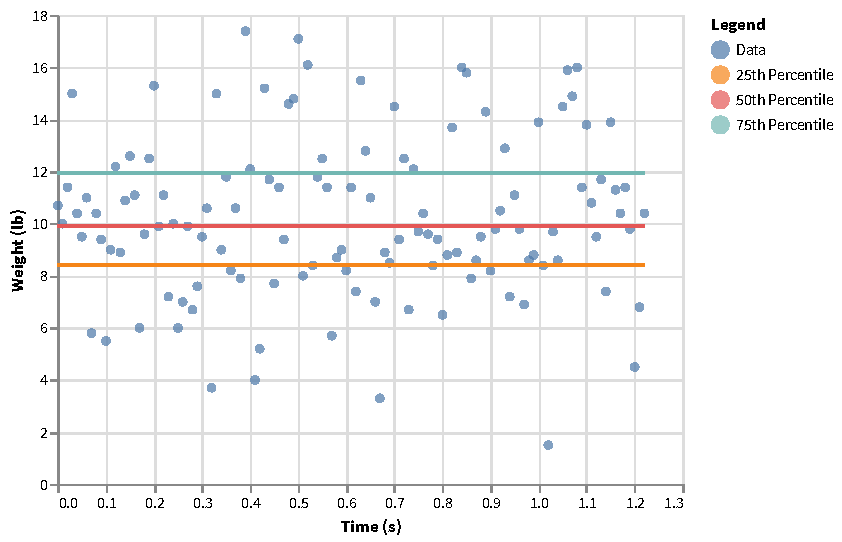
\includegraphics{chart/00-intro/baseline-quartiles.pdf}
    \caption{Quartiles for Baseline Segment}
    \label{figure:00.baseline.quartiles}
\end{figure}
%
\begin{figure}[ht]
    \centering
    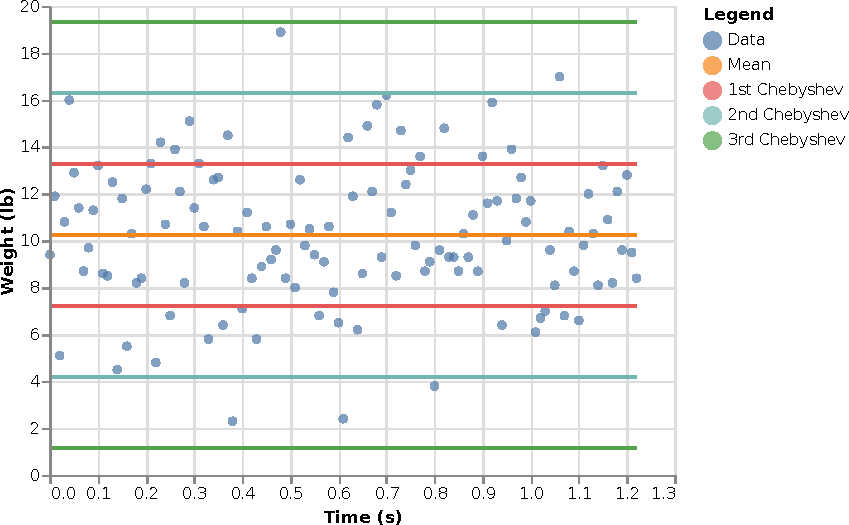
\includegraphics{chart/00-intro/baseline-chebyshev.pdf}
    \caption{Three Chebyshev Intervals for Baseline Segment}
    \label{figure:00.baseline.chebyshev}
\end{figure}
%
\begin{figure}[ht]
    \centering
    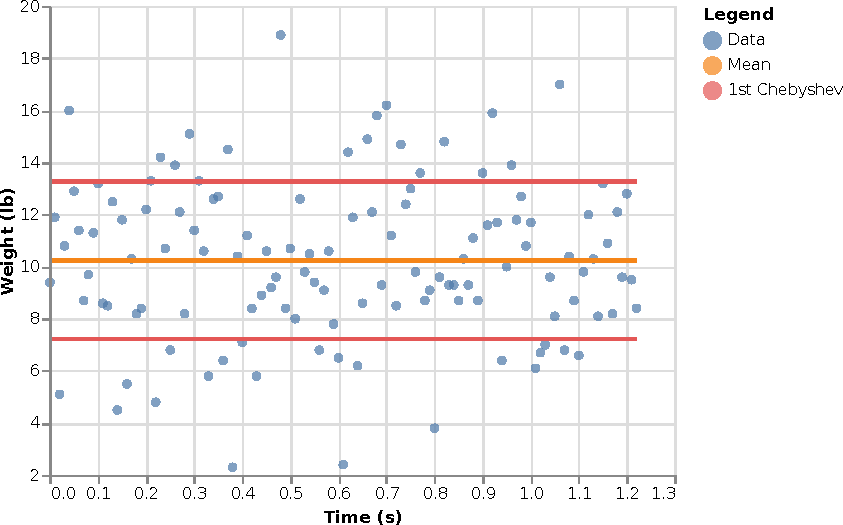
\includegraphics{chart/00-intro/baseline-chebyshev-1.pdf}
    \caption{First Chebyshev Interval for Baseline Segment}
    \label{figure:00.baseline.chebyshev.1}
\end{figure}
%
\begin{figure}[ht]
    \centering
    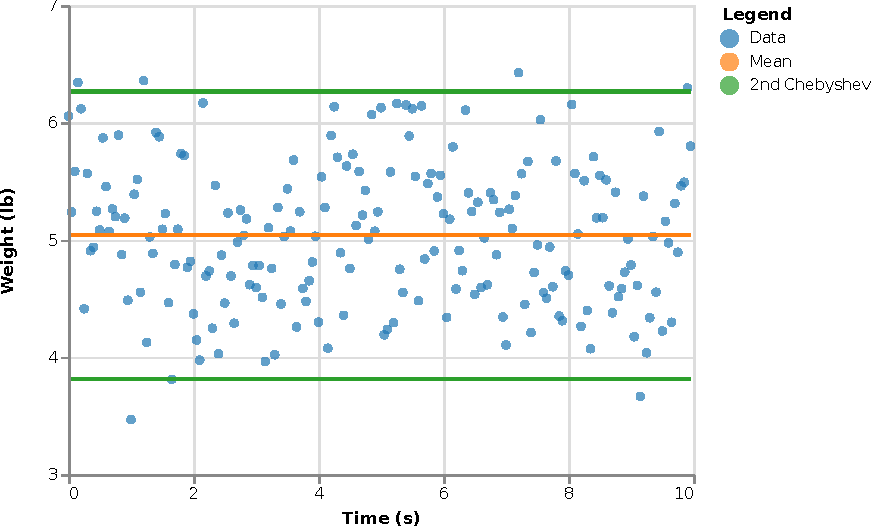
\includegraphics{chart/00-intro/baseline-chebyshev-2.pdf}
    \caption{Second Chebyshev Interval for Baseline Segment}
    \label{figure:00.baseline.chebyshev.2}
\end{figure}
%
\begin{figure}[ht]
    \centering
    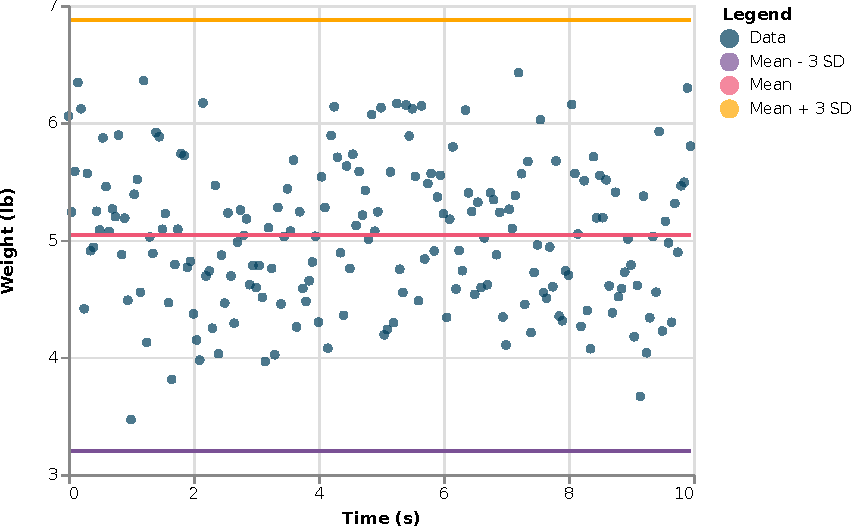
\includegraphics{chart/00-intro/baseline-chebyshev-3.pdf}
    \caption{Third Chebyshev Interval for Baseline Segment}
    \label{figure:00.baseline.chebyshev.3}
\end{figure}
%
\begin{figure}[ht]
    \centering
    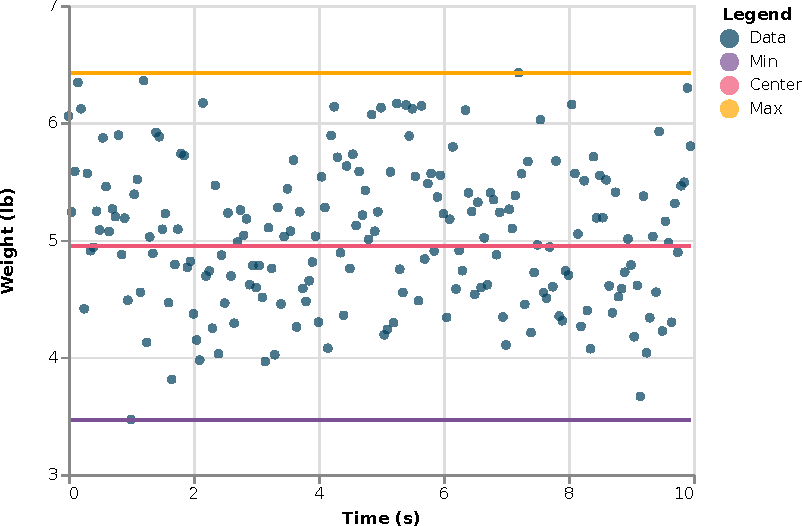
\includegraphics{chart/00-intro/baseline-min-center-max.pdf}
    \caption{Range and Center for Baseline Segment}
    \label{figure:00.baseline.center}
\end{figure}
%
\begin{figure}[ht]
    \centering
    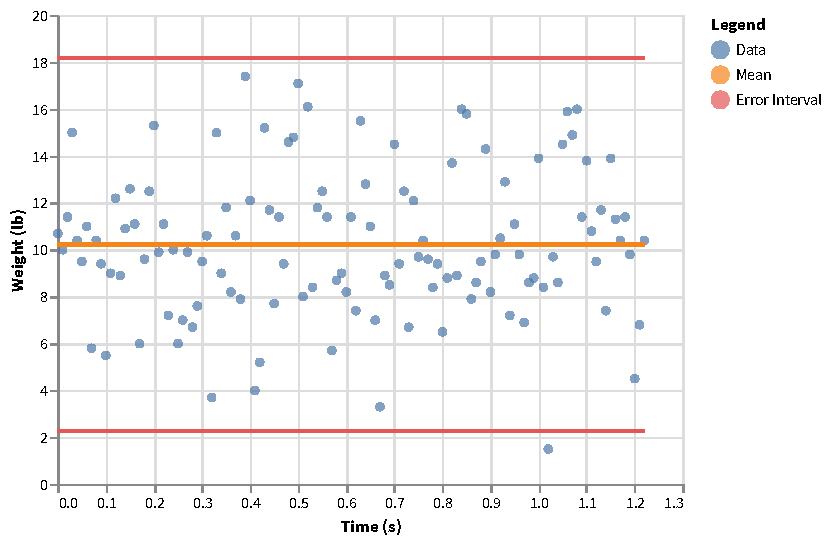
\includegraphics{chart/00-intro/baseline-error-interval.pdf}
    \caption{Error Interval for Baseline Segment}
    \label{figure:00.baseline.interval}
\end{figure}
%
\begin{figure}[ht]
    \centering
    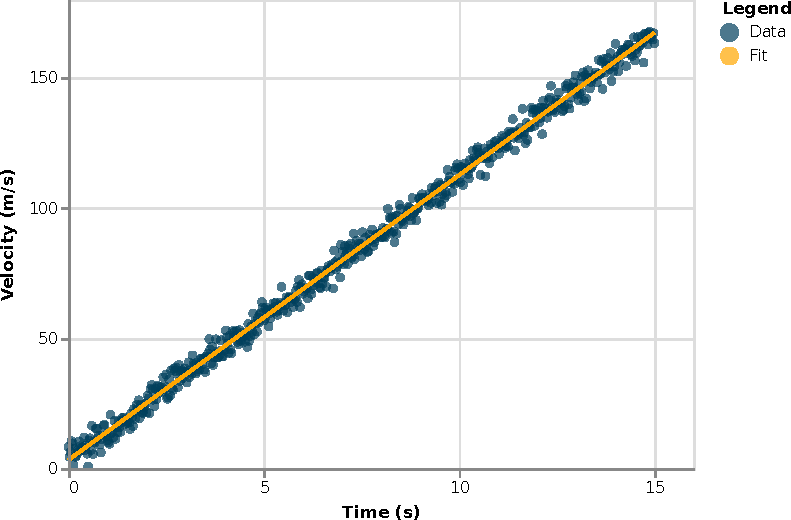
\includegraphics{chart/00-intro/velocity-fit.pdf}
    \caption{Velocity Data and Best Fit}
    \label{figure:00.velocity.fit}
\end{figure}
%

\part{Constant Acceleration}
% Copyright 2018 Melvin Eloy Irizarry-Gelpí
\setcounter{chapter}{1}
\chapter{Error Analysis}
%%%%%%%%%%%%%%%%%%%%%%%%%%%%%%%%%%%%%%%%%%%%%%%%%%%%%%%%%%%%%%%%%%%%%%%%%%%%%%%%
In this experiment you will learn about error analysis and provide an estimate for the acceleration of a free-falling object under the influence of gravity.
%%%%%%%%%%%%%%%%%%%%%%%%%%%%%%%%%%%%%%%%%%%%%%%%%%%%%%%%%%%%%%%%%%%%%%%%%%%%%%%%
\section{Preliminary}
%%%%%%%%%%%%%%%%%%%%%%%%%%%%%%%%%%%%%%%%%%%%%%%%%%%%%%%%%%%%%%%%%%%%%%%%%%%%%%%%
Ignoring the effects of air resistance, when an object is dropped and falls a certain height, its velocity is proportional to the amount of travel time. The slope in the linear relation corresponds to the free-fall acceleration. Since this acceleration is due to gravity, its value is usually denoted by $g$. On Earth, near sea level, the value of $g$ is 9.80 m/s$^{2}$.

Here velocity is measured in meters per second (m/s), and time is measured in seconds (s). A linear relation between velocity $v$ and time $t$ has the mathematical form
\begin{equation}
    v = A t + B
\end{equation}
Here $A$ is the \textbf{slope} and $B$ is the \textbf{intercept}. Both $A$ and $B$ will also have units. Indeed, $A$ must have units of meters per second per second (m/s/s or m/s$^{2}$) and $B$ must have units of meters per second (m/s). Thus, the slope should have units of \textbf{acceleration}, and the intercept should have units of \textbf{velocity}.
%%%%%%%%%%%%%%%%%%%%%%%%%%%%%%%%%%%%%%%%%%%%%%%%%%%%%%%%%%%%%%%%%%%%%%%%%%%%%%%%
\section{Experiment}
%%%%%%%%%%%%%%%%%%%%%%%%%%%%%%%%%%%%%%%%%%%%%%%%%%%%%%%%%%%%%%%%%%%%%%%%%%%%%%%%
You use a photogate to measure the velocity over time of a picket fence that falls freely. Then you use the LabQuest device to easily find the equation for the line that best fits the experimental data.

First you considered 5 runs. For each run, you dropped the picket fence from increasingly higher starting positions. You recorded both the slope and the intercept.

Then you considered 25 runs. For these runs, you always dropped the picket fence from just above the photogate. You recorded only the slope. In the end you should have a total of 30 values for the slope.
%%%%%%%%%%%%%%%%%%%%%%%%%%%%%%%%%%%%%%%%%%%%%%%%%%%%%%%%%%%%%%%%%%%%%%%%%%%%%%%%
\section{Analysis}
%%%%%%%%%%%%%%%%%%%%%%%%%%%%%%%%%%%%%%%%%%%%%%%%%%%%%%%%%%%%%%%%%%%%%%%%%%%%%%%%
You can divide the analysis into five parts.
%%%%%%%%%%%%%%%%%%%%%%%%%%%%%%%%%%%%%%%%%%%%%%%%%%%%%%%%%%%%%%%%%%%%%%%%%%%%%%%%
\subsection{First 5 Runs} \label{sec:01.first.5}
%%%%%%%%%%%%%%%%%%%%%%%%%%%%%%%%%%%%%%%%%%%%%%%%%%%%%%%%%%%%%%%%%%%%%%%%%%%%%%%%
For the first 5 runs, you recorded \textbf{both the slope and the intercept} values of the best-fit line. Here are some questions:
\begin{enumerate}
    \item Are the \textbf{slope} values for different heights all close in magnitude? Explain the physical consequences of your observation.
    \item Are the \textbf{intercept} values for different heights all close in magnitude? Explain the physical consequences of your observation.
    \item What is the smallest slope value (i.e. the \textbf{minimum}) recorded? Use the \texttt{MIN} function (see Equation \ref{eq:00.min}).
    \item What is the \textbf{median} slope value? Use the \texttt{MEDIAN} function (see Equation \ref{eq:00.median}).
    \item What is the largest slope value (i.e. the \textbf{maximum}) recorded? Use the \texttt{MAX} function (see Equation \ref{eq:00.max}).
    \item What is the \textbf{average} slope value? Use the \texttt{AVERAGE} function (see Equation \ref{eq:00.average}).
    \item What is the \textbf{percent difference} between the expected value for the slope (9.80 m/s$^{2}$) and the 5-run average? See Equation \ref{eq:00.percent.diff}.
\end{enumerate}
%%%%%%%%%%%%%%%%%%%%%%%%%%%%%%%%%%%%%%%%%%%%%%%%%%%%%%%%%%%%%%%%%%%%%%%%%%%%%%%%
\subsection{Latter 25 Runs} \label{sec:01.latter.25}
%%%%%%%%%%%%%%%%%%%%%%%%%%%%%%%%%%%%%%%%%%%%%%%%%%%%%%%%%%%%%%%%%%%%%%%%%%%%%%%%
For the latter 25 runs, you recorded \textbf{only the slope}. Here are some questions:
\begin{enumerate}
    \item What is the minimum slope value recorded?
    \item What is the median slope value?
    \item What is the maximum slope value recorded?
    \item What is the average slope value?
    \item Are the answers to these questions similar to the answers for the first 5 runs?
    \item What is the percent difference between the expected value for the slope (9.80 m/s$^{2}$) and the 25-run average?
\end{enumerate}
%%%%%%%%%%%%%%%%%%%%%%%%%%%%%%%%%%%%%%%%%%%%%%%%%%%%%%%%%%%%%%%%%%%%%%%%%%%%%%%%
\subsection{Aggregate of 30 Runs} \label{sec:01.all.30}
%%%%%%%%%%%%%%%%%%%%%%%%%%%%%%%%%%%%%%%%%%%%%%%%%%%%%%%%%%%%%%%%%%%%%%%%%%%%%%%%
You can combine the first 5 runs with the latter 25 runs and make a 30-run aggregate. You can ask similar questions:
\begin{enumerate}
    \item What is the minimum slope value recorded?
    \item What is the \textbf{25th percentile} slope value? Use the \texttt{PERCENTILE} function (see Equation \ref{eq:00.percentile.25}).
    \item What is the \textbf{50th percentile} slope value? Use the \texttt{PERCENTILE} function (see Equation \ref{eq:00.percentile.50}).
    \item What is the \textbf{75th percentile} slope value? Use the \texttt{PERCENTILE} function (see Equation \ref{eq:00.percentile.75}).
    \item What is the maximum slope value recorded?
    \item What is the \textbf{error} (see Equation \ref{eq:00.error})?
    \item What is the average slope?
    \item What are the boundaries of the \textbf{error interval} (i.e. \texttt{AVERAGE} $\pm$ \texttt{ERROR})?
    \item What is the percent difference between the expected value for the slope (9.80 m/s$^{2}$) and the 30-run average?
\end{enumerate}
%%%%%%%%%%%%%%%%%%%%%%%%%%%%%%%%%%%%%%%%%%%%%%%%%%%%%%%%%%%%%%%%%%%%%%%%%%%%%%%%
\subsection{Central 20 Runs} \label{sec:01.central.20}
%%%%%%%%%%%%%%%%%%%%%%%%%%%%%%%%%%%%%%%%%%%%%%%%%%%%%%%%%%%%%%%%%%%%%%%%%%%%%%%%
You can take the 30-run aggregate, sort the values in either increasing or decreasing order, and then drop the \textbf{smallest} 5 values, and also the \textbf{largest} 5 values. After doing this you remain with \textbf{20 values}, corresponding to the 20 runs that are most ``central''. That is, the 20 values that are neither the smallest nor the largest. Note that 20 out of 30 is the same as 2/3 of the data set (66\%).

Here is how to sort a column with Google Sheets. If \texttt{Aggregate30} is the name of the named range with the 30 slope values, then, in a separate sheet use
\begin{equation}
    \texttt{=SORT(Aggregate30, 1, TRUE)}
\end{equation}
If there is enough space, you should see the 30 slope values appear but in ascending order (smallest to largest). Using \texttt{FALSE} instead of \texttt{TRUE} will give you the slopes in descending order (largest to smallest).

After dropping the bottom 5 and top 5, you can answer the following questions:
\begin{enumerate}
    \item What is the minimum slope value for these 20 runs?
    \item What is the average slope value for these 20 runs?
    \item What is the maximum slope value for these 20 runs?
    \item What is the error?
    \item What is the percent difference between the expected value for the slope (9.80 m/s$^{2}$) and the (central) 20-run average?
\end{enumerate} 
%%%%%%%%%%%%%%%%%%%%%%%%%%%%%%%%%%%%%%%%%%%%%%%%%%%%%%%%%%%%%%%%%%%%%%%%%%%%%%%%
\subsection{Closest 20 Runs} \label{sec:01.closest.20}
%%%%%%%%%%%%%%%%%%%%%%%%%%%%%%%%%%%%%%%%%%%%%%%%%%%%%%%%%%%%%%%%%%%%%%%%%%%%%%%%
Instead of looking at the central 2/3 of the data, you can look at the 2/3 of the data that is \textbf{closest} to the 30-run average. Proximity requires a notion of distance. In our case we can define the distance between the slope value $g_{j}$ and the 30-run average slope $g_{A}$ as
\begin{equation}
    \text{distance} = \vert g_{j} - g_{A} \vert
\end{equation}
The absolute value will remove the signs in the difference and account for the slope being less or greater than the average. Keeping the closest 20 values amounts to dropping the 10 values that are farthest away (i.e. with the largest amount of distance from the average). Thus, you compute the distance from average in a column, then sort this column, then drop the 10 values farthest away from the average.

Here is a more detailed list of steps to follow:
\begin{enumerate}
    \item Copy and paste the slopes for the 30-run aggregate. The slope values should be in \texttt{column A}, from \texttt{row 2} to \texttt{row 31}.
    \item Copy and paste the average slope value for the 30-run aggregate. In my case, I pasted it on cell \texttt{E15} (i.e. \texttt{column E} and \texttt{row 15}).
    \item In \texttt{column B}, compute the distance from the first slope value to the 30-run average with the following equation:
    \begin{equation}
        \texttt{=ABS(A2 - E\$15)}
    \end{equation}
    Note the \textbf{dollar sign} in the second term, which is needed.
    \item Click on cell \texttt{B2}, hold \texttt{Shift} down and select the rest of the column values down until \texttt{row 31}. Press both \texttt{Ctrl} and \texttt{D} keys (or both \texttt{Cmd} and \texttt{D} keys in Mac OSX). This should apply the distance equation to the entire column. You should have the slope values on \texttt{column A}, and the distance values on \texttt{column B}.
    \item Make a named range with the distance values. I used \texttt{DistanceToAverage30}.
    \item Now you want to sort the distance column, but you also want the sorting to be applied to the slope column. In order to do this, find a region in a sheet with enough space for two columns of 30 values each. Click on the top left cell of this region and use
    \begin{equation}
        \texttt{=SORT({Aggregate30,DistanceToAverage30}, 2, FALSE)}
    \end{equation}
    You should see the 30 slope values appear in one column, and the 30 distance values appear in the second column, but the distance column will be sorted in descending order. The top 10 values correspond to the 10 values that are farthest away from the 30-run average. The other 20 values constitute the closest 20 runs.
\end{enumerate}
After doing this, you can answer the following questions:
\begin{enumerate}
    \item What is the minimum slope value for these 20 runs?
    \item What is the maximum slope value for these 20 runs?
    \item What is the error?
    \item What is the average slope value for these 20 runs?
    \item What is the percent difference between the expected value for the slope (9.80 m/s$^{2}$) and the (closest) 20-run average?
\end{enumerate}
%%%%%%%%%%%%%%%%%%%%%%%%%%%%%%%%%%%%%%%%%%%%%%%%%%%%%%%%%%%%%%%%%%%%%%%%%%%%%%%%
\section{My Data}
%%%%%%%%%%%%%%%%%%%%%%%%%%%%%%%%%%%%%%%%%%%%%%%%%%%%%%%%%%%%%%%%%%%%%%%%%%%%%%%%
The data for my first 5 runs are in Table \ref{table:01.first.5}. The data for my latter 25 runs are in Table \ref{table:01.latter.25}.

In Table \ref{table:01.describe.5} and Table \ref{table:01.describe.25}, I describe the raw data. Note that, in my case, the average slope is much larger, and also much closer to the actual value, for the 25 runs.

After combining all the runs into the 30-run aggregate, you can consider other quantities like the percentiles. In Table \ref{table:01.describe.30} you can find the three percentiles, as well as the previous quantities that were also found in the first two parts. The boundaries of the error interval for the 30-run aggregate are found in Table \ref{table:01.error.30}. Note that the established value for the slope, 9.80 m/s$^{2}$ is inside of the error interval.

The minimum slope for the 30-run aggregate is quite small and could be an outlier. One way to deal with outliers is to restrict to a subset of the data. To be clear: You do not get to choose which values to keep or which values to drop based on their proximity to the expected value. That would be cheating. It would introduce bias to your data. Besides, in most experiments, you do not know the expected value. Instead you can restrict to a subset of the data by following an explicit rule intrinsic to the data.

In Table \ref{table:01.describe.20.center} you can find the statistics for the subset of the data that correspond to the 2/3 that is in the middle: neither the smallest nor the largest. To keep this fair, you need to drop the same amount of small values as you drop large values. In my case I calculated again the same quantities in Table \ref{table:01.describe.30} for the 30-run aggregate, but you do not have to find everything. Just the minimum, maximum, average, and error. Note that the error value for the central 20 runs is smaller than the error for the 30-run average. For the central 20 runs, the expected value still falls inside the error interval.

Instead of the central 2/3, you can keep the 2/3 that is closest to the 30-run average. In Table \ref{table:01.describe.20.close} and Table \ref{table:01.error.20.close} you can find the analogous results for this case. Note that for my data, the error happens to be smaller for the closest 20 runs than for the central 20 runs.

Finally, Table \ref{table:01.summary} has the comparisons of the different averages to the expected value, in the form of percent difference. In my case, the least error was found for the closest 20 runs. Your results might be different.
%%%%%%%%%%%%%%%%%%%%%%%%%%%%%%%%%%%%%%%%%%%%%%%%%%%%%%%%%%%%%%%%%%%%%%%%%%%%%%%%
\section{Your Data}
%%%%%%%%%%%%%%%%%%%%%%%%%%%%%%%%%%%%%%%%%%%%%%%%%%%%%%%%%%%%%%%%%%%%%%%%%%%%%%%%
Your data should consist of 5 initial pairs of slope and intercept values, plus 25 additional slope values. In total you should have 30 slopes and 5 intercepts.
%%%%%%%%%%%%%%%%%%%%%%%%%%%%%%%%%%%%%%%%%%%%%%%%%%%%%%%%%%%%%%%%%%%%%%%%%%%%%%%%
\newpage
\section{Your Laboratory Report}
%%%%%%%%%%%%%%%%%%%%%%%%%%%%%%%%%%%%%%%%%%%%%%%%%%%%%%%%%%%%%%%%%%%%%%%%%%%%%%%%
Your laboratory report should include the following:
\begin{itemize}
    \item Tables like Table \ref{table:01.first.5} and \ref{table:01.latter.25} with your raw data. This is one of the few experiments where you can include the raw data in your report.
    \item Answers to all the questions in Section \ref{sec:01.first.5} (some in a table like Table \ref{table:01.describe.5}).
    \item Answers to all the questions in Section \ref{sec:01.latter.25} (some in a table like Table \ref{table:01.describe.25}).
    \item Answers to all the questions in Section \ref{sec:01.all.30} (some in tables like Tables \ref{table:01.describe.30} and \ref{table:01.error.30}).
    \item Answers to all the questions in Section \ref{sec:01.central.20} (some in tables like Tables \ref{table:01.describe.20.center} and \ref{table:01.error.20.center}).
    \item Answers to all the questions in Section \ref{sec:01.closest.20} (some in tables like Tables \ref{table:01.describe.20.close} and \ref{table:01.error.20.close}).
    \item Compare your average slope values to the expected value by calculating percent differences as in Table \ref{table:01.summary}.
\end{itemize}
You should answer the following questions:
\begin{enumerate}
    \item Given two ways to keep 2/3 of the data (central 20 runs or closest 20 runs), which approach do you think yields the most confident or robust result? Why?
    \item Out of Sections \ref{sec:01.all.30}, \ref{sec:01.central.20}, and \ref{sec:01.closest.20}, which part had the largest/smallest amount of error?
    \item Which of your estimates is closest to the expected value?
\end{enumerate}
%%%%%%%%%%%%%%%%%%%%%%%%%%%%%%%%%%%%%%%%%%%%%%%%%%%%%%%%%%%%%%%%%%%%%%%%%%%%%%%%
\FloatBarrier
\newpage
\section{Tables}
%%%%%%%%%%%%%%%%%%%%%%%%%%%%%%%%%%%%%%%%%%%%%%%%%%%%%%%%%%%%%%%%%%%%%%%%%%%%%%%%
\begin{table}[ht]
    \centering
    \begin{tabular}{|r|r|}
        \hline
        \textbf{Slope} (m/s$^{2}$) & \textbf{Intercept} (m/s) \\
        \hline
        9.4265 & 0.8407 \\
        9.7359 & 1.2777 \\
        9.2793 & 1.9661 \\
        9.7066 & 2.6893 \\
        9.7122 & 3.1737 \\
        \hline
    \end{tabular}
    \caption{First 5 runs}
    \label{table:01.first.5}
\end{table}
%%%%%%%%%%%%%%%%%%%%%%%%%%%%%%%%%%%%%%%%%%%%%%%%%%%%%%%%%%%%%%%%%%%%%%%%%%%%%%%%
\begin{table}[ht]
    \centering
    \begin{tabular}{|r|r|r|r|r|}
        \hline
        9.7839 & 9.586 & 9.5585 & 9.5695 & 9.8151 \\
        \hline
        9.779 & 9.7948 & 9.7412 & 9.7468 & 9.7604 \\
        \hline
        9.7961 & 9.5095 & 9.628 & 9.7107 & 9.7363 \\
        \hline
        9.7065 & 9.6901 & 9.8093 & 9.8058 & 9.7818 \\
        \hline
        9.7677 & 9.7252 & 9.7621 & 9.7566 & 9.6849 \\
        \hline
    \end{tabular}
    \caption{Slope values for latter 25 runs, in units of m/s$^{2}$}
    \label{table:01.latter.25}
\end{table}
%%%%%%%%%%%%%%%%%%%%%%%%%%%%%%%%%%%%%%%%%%%%%%%%%%%%%%%%%%%%%%%%%%%%%%%%%%%%%%%%
\begin{table}[ht]
    \centering
    \begin{tabular}{|l|r|}
        \hline
        \textbf{Name} & \textbf{Value} (m/s$^{2}$) \\
        \hline
        Minimum & 9.2793 \\
        Median & 9.7066 \\
        Maximum & 9.7359 \\
        Average & 9.5721 \\
        \hline
    \end{tabular}
    \caption{Min, average, and max for first 5 runs}
    \label{table:01.describe.5}
\end{table}
%%%%%%%%%%%%%%%%%%%%%%%%%%%%%%%%%%%%%%%%%%%%%%%%%%%%%%%%%%%%%%%%%%%%%%%%%%%%%%%%
\begin{table}[ht]
    \centering
    \begin{tabular}{|l|r|}
        \hline
        \textbf{Name} & \textbf{Value} (m/s$^{2}$) \\
        \hline
        Minimum & 9.5095 \\
        Median & 9.7468 \\
        Maximum & 9.8151 \\
        Average & 9.7202 \\
        \hline
    \end{tabular}
    \caption{Min, average, and max for latter 25 runs}
    \label{table:01.describe.25}
\end{table}
%%%%%%%%%%%%%%%%%%%%%%%%%%%%%%%%%%%%%%%%%%%%%%%%%%%%%%%%%%%%%%%%%%%%%%%%%%%%%%%%
\begin{table}[ht]
    \centering
    \begin{tabular}{|l|r|}
        \hline
        \textbf{Name} & \textbf{Value} (m/s$^{2}$) \\
        \hline
        Minimum & 9.2793 \\
        25th Percentile & 9.6862 \\
        50th Percentile & 9.7361 \\
        75th Percentile & 9.7762 \\
        Maximum & 9.8151 \\
        Error & 0.2679 \\
        \hline
    \end{tabular}
    \caption{Min, quartiles, max, and error for 30-run aggregate}
    \label{table:01.describe.30}
\end{table}
%%%%%%%%%%%%%%%%%%%%%%%%%%%%%%%%%%%%%%%%%%%%%%%%%%%%%%%%%%%%%%%%%%%%%%%%%%%%%%%%
\begin{table}[ht]
    \centering
    \begin{tabular}{|l|r|}
        \hline
        \textbf{Name} & \textbf{Value} (m/s$^{2}$) \\
        \hline
        Average - Error & 9.4276 \\
        Average & 9.6955 \\
        Average + Error & 9.9634 \\
        \hline
    \end{tabular}
    \caption{Error interval for 30-run aggregate}
    \label{table:01.error.30}
\end{table}
%%%%%%%%%%%%%%%%%%%%%%%%%%%%%%%%%%%%%%%%%%%%%%%%%%%%%%%%%%%%%%%%%%%%%%%%%%%%%%%%
\begin{table}[ht]
    \centering
    \begin{tabular}{|l|r|}
        \hline
        \textbf{Name} & \textbf{Value} (m/s$^{2}$) \\
        \hline
        Minimum & 9.586 \\
        25th Percentile & 9.7066 \\
        50th Percentile & 9.7361 \\
        75th Percentile & 9.7608 \\
        Maximum & 9.7839 \\
        Error & 0.0989 \\
        \hline
    \end{tabular}
    \caption{Min, quartiles, max, and error for central 20 runs}
    \label{table:01.describe.20.center}
\end{table}
%%%%%%%%%%%%%%%%%%%%%%%%%%%%%%%%%%%%%%%%%%%%%%%%%%%%%%%%%%%%%%%%%%%%%%%%%%%%%%%%
\begin{table}[ht]
    \centering
    \begin{tabular}{|l|r|}
        \hline
        \textbf{Name} & \textbf{Value} (m/s$^{2}$) \\
        \hline
        Average - Error & 9.6261 \\
        Average & 9.7251 \\
        Average + Error & 9.8240 \\
        \hline
    \end{tabular}
    \caption{Error interval for central 20 runs}
    \label{table:01.error.20.center}
\end{table}
%%%%%%%%%%%%%%%%%%%%%%%%%%%%%%%%%%%%%%%%%%%%%%%%%%%%%%%%%%%%%%%%%%%%%%%%%%%%%%%%
\begin{table}[ht]
    \centering
    \begin{tabular}{|l|r|}
        \hline
        \textbf{Name} & \textbf{Value} (m/s$^{2}$) \\
        \hline
        Minimum & 9.628 \\
        25th Percentile & 9.7097 \\
        50th Percentile & 9.7388 \\
        75th Percentile & 9.7635 \\
        Maximum & 9.7948 \\
        Error & 0.0834 \\
        \hline
    \end{tabular}
    \caption{Min, quartiles, max, and error for closest 20 runs}
    \label{table:01.describe.20.close}
\end{table}
%%%%%%%%%%%%%%%%%%%%%%%%%%%%%%%%%%%%%%%%%%%%%%%%%%%%%%%%%%%%%%%%%%%%%%%%%%%%%%%%
\begin{table}[ht]
    \centering
    \begin{tabular}{|l|r|}
        \hline
        \textbf{Name} & \textbf{Value} (m/s$^{2}$) \\
        \hline
        Average - Error & 9.6521 \\
        Average & 9.7355 \\
        Average + Error & 9.8189 \\
        \hline
    \end{tabular}
    \caption{Error interval for closest 20 runs}
    \label{table:01.error.20.close}
\end{table}
%%%%%%%%%%%%%%%%%%%%%%%%%%%%%%%%%%%%%%%%%%%%%%%%%%%%%%%%%%%%%%%%%%%%%%%%%%%%%%%%
\begin{table}[ht]
    \centering
    \begin{tabular}{|l|r|r|r|r|}
        \hline
        \textbf{Name} & \textbf{Error} (m/s$^{2}$) & \textbf{Experimental} (m/s$^{2}$) & \textbf{Theoretical} (m/s$^{2}$) & \textbf{P.D.} \\
        \hline
        First 5 & 0.2283 & 9.5721 & 9.8 & -2.33\% \\
        Latter 25 & 0.1528 & 9.7202 & 9.8 & -0.81\% \\
        Aggregate 30 & 0.2679 & 9.6955 & 9.8 & -1.07\% \\
        Center 20 & 0.0989 & 9.7251 & 9.8 & -0.76\% \\
        Closest 20 & 0.0834 & 9.7355 & 9.8 & -0.66\% \\
        \hline
    \end{tabular}
    \caption{Summary of results and percent differences}
    \label{table:01.summary}
\end{table}
%%%%%%%%%%%%%%%%%%%%%%%%%%%%%%%%%%%%%%%%%%%%%%%%%%%%%%%%%%%%%%%%%%%%%%%%%%%%%%%%

% Copyright 2018 Melvin Eloy Irizarry-Gelpí
\chapter{Motion on an Incline}
%%%%%%%%%%%%%%%%%%%%%%%%%%%%%%%%%%%%%%%%%%%%%%%%%%%%%%%%%%%%%%%%%%%%%%%%%%%%%%%%
...
%%%%%%%%%%%%%%%%%%%%%%%%%%%%%%%%%%%%%%%%%%%%%%%%%%%%%%%%%%%%%%%%%%%%%%%%%%%%%%%%
\section{Preliminary}
%%%%%%%%%%%%%%%%%%%%%%%%%%%%%%%%%%%%%%%%%%%%%%%%%%%%%%%%%%%%%%%%%%%%%%%%%%%%%%%%
...
%%%%%%%%%%%%%%%%%%%%%%%%%%%%%%%%%%%%%%%%%%%%%%%%%%%%%%%%%%%%%%%%%%%%%%%%%%%%%%%%
\section{Experiment}
%%%%%%%%%%%%%%%%%%%%%%%%%%%%%%%%%%%%%%%%%%%%%%%%%%%%%%%%%%%%%%%%%%%%%%%%%%%%%%%%
...
%%%%%%%%%%%%%%%%%%%%%%%%%%%%%%%%%%%%%%%%%%%%%%%%%%%%%%%%%%%%%%%%%%%%%%%%%%%%%%%%
\section{Analysis}
%%%%%%%%%%%%%%%%%%%%%%%%%%%%%%%%%%%%%%%%%%%%%%%%%%%%%%%%%%%%%%%%%%%%%%%%%%%%%%%%
...
%%%%%%%%%%%%%%%%%%%%%%%%%%%%%%%%%%%%%%%%%%%%%%%%%%%%%%%%%%%%%%%%%%%%%%%%%%%%%%%%
\section{My Data}
%%%%%%%%%%%%%%%%%%%%%%%%%%%%%%%%%%%%%%%%%%%%%%%%%%%%%%%%%%%%%%%%%%%%%%%%%%%%%%%%
...
%%%%%%%%%%%%%%%%%%%%%%%%%%%%%%%%%%%%%%%%%%%%%%%%%%%%%%%%%%%%%%%%%%%%%%%%%%%%%%%%
\section{Your Data}
%%%%%%%%%%%%%%%%%%%%%%%%%%%%%%%%%%%%%%%%%%%%%%%%%%%%%%%%%%%%%%%%%%%%%%%%%%%%%%%%
...
%%%%%%%%%%%%%%%%%%%%%%%%%%%%%%%%%%%%%%%%%%%%%%%%%%%%%%%%%%%%%%%%%%%%%%%%%%%%%%%%
\section{Your Lab Report}
%%%%%%%%%%%%%%%%%%%%%%%%%%%%%%%%%%%%%%%%%%%%%%%%%%%%%%%%%%%%%%%%%%%%%%%%%%%%%%%%
...
\part{Force}
% Copyright 2018 Melvin Eloy Irizarry-Gelpí
\setcounter{chapter}{2}
\chapter{Newton's First Law}
%%%%%%%%%%%%%%%%%%%%%%%%%%%%%%%%%%%%%%%%%%%%%%%%%%%%%%%%%%%%%%%%%%%%%%%%%%%%%%%%
In this experiment you will check Newton's first law of motion by considering the effects of diminishing amounts of friction.
%%%%%%%%%%%%%%%%%%%%%%%%%%%%%%%%%%%%%%%%%%%%%%%%%%%%%%%%%%%%%%%%%%%%%%%%%%%%%%%%
\section{Preliminary}
%%%%%%%%%%%%%%%%%%%%%%%%%%%%%%%%%%%%%%%%%%%%%%%%%%%%%%%%%%%%%%%%%%%%%%%%%%%%%%%%
Newton's \textbf{first law of motion} states that
\begin{itemize}
    \item an object in uniform linear motion will remain in uniform linear motion unless acted by an external (net) force.
\end{itemize}
\textbf{Uniform linear motion} is motion where the \textbf{velocity is constant}. Recall that velocity is a vector physical quantity: velocity has a \textbf{magnitude} (speed) and a \textbf{direction}. If an object moves with constant velocity, then both the magnitude and the direction are fixed in time. If there is an external net force acting on the object, then the velocity will change with time due to this force, and the motion will not be uniform linear motion.

If velocity is constant, then it is not changing with time. Thus, when velocity is constant, the rate of change of velocity with time is zero. But acceleration is defined as the rate of change of velocity with time. Thus, an object in uniform linear motion will have zero acceleration.

Friction is an ubiquitous force. It is almost always present in most motions. There are many kinds of frictional forces, but the most relevant one for this experiment is \textbf{kinetic friction}. The most important aspect of kinetic friction is that it is approximately constant in magnitude, and directly proportional to the amount of normal force on the surface. Later you will learn that a \textbf{constant net force} leads to a \textbf{constant acceleration}. You have done two experiments with constant acceleration: the free-falling picket fence and the cart moving along an incline. In both of this you learned that the value of the constant acceleration can be learned from the slope of the velocity versus time chart.
%%%%%%%%%%%%%%%%%%%%%%%%%%%%%%%%%%%%%%%%%%%%%%%%%%%%%%%%%%%%%%%%%%%%%%%%%%%%%%%%
\section{Experiment}
%%%%%%%%%%%%%%%%%%%%%%%%%%%%%%%%%%%%%%%%%%%%%%%%%%%%%%%%%%%%%%%%%%%%%%%%%%%%%%%%
You use a motion sensor to measure the position, velocity, and acceleration of a cart. The cart has a mechanism that allows kinetic friction to be adjusted. You consider motions along a track with increasing amounts of kinetic friction, and extrapolate your results to verify that Newton's first law of motion is indeed correct.
%%%%%%%%%%%%%%%%%%%%%%%%%%%%%%%%%%%%%%%%%%%%%%%%%%%%%%%%%%%%%%%%%%%%%%%%%%%%%%%%
\section{Analysis}
%%%%%%%%%%%%%%%%%%%%%%%%%%%%%%%%%%%%%%%%%%%%%%%%%%%%%%%%%%%%%%%%%%%%%%%%%%%%%%%%
For this experiment you are only going to analyze the velocity and time data. Here are some steps to follow for each run:
\begin{enumerate}
    \item Make a scatter chart with velocity in the vertical axis and time in the horizontal axis.
    \item Restrict to the region where the shape is appropriately linear. This might involve deleting data from the beginning and/or the end.
    \item Once the linear segment is the only part remaining, add a best-fit line and record the value of the intercept and the slope.
\end{enumerate}
%%%%%%%%%%%%%%%%%%%%%%%%%%%%%%%%%%%%%%%%%%%%%%%%%%%%%%%%%%%%%%%%%%%%%%%%%%%%%%%%
\section{My Data}
%%%%%%%%%%%%%%%%%%%%%%%%%%%%%%%%%%%%%%%%%%%%%%%%%%%%%%%%%%%%%%%%%%%%%%%%%%%%%%%%
My data consist of eight runs. For run 1 the friction pad was retracted all the way. For runs 2, 3, and 4 the friction pad was brought closer to the track, but the effect was not noticeable on the slope. Starting with run 5, you see the effects of the friction pad change the value of the slope. Run 8 is when the friction pad is at its lowest configuration.
%%%%%%%%%%%%%%%%%%%%%%%%%%%%%%%%%%%%%%%%%%%%%%%%%%%%%%%%%%%%%%%%%%%%%%%%%%%%%%%%
\section{Your Data}
%%%%%%%%%%%%%%%%%%%%%%%%%%%%%%%%%%%%%%%%%%%%%%%%%%%%%%%%%%%%%%%%%%%%%%%%%%%%%%%%
You should have about 6 runs of data with the friction pad close to the track, and one run with the friction pad not touching the track.
%%%%%%%%%%%%%%%%%%%%%%%%%%%%%%%%%%%%%%%%%%%%%%%%%%%%%%%%%%%%%%%%%%%%%%%%%%%%%%%%
\newpage
\section{Your Laboratory Report}
%%%%%%%%%%%%%%%%%%%%%%%%%%%%%%%%%%%%%%%%%%%%%%%%%%%%%%%%%%%%%%%%%%%%%%%%%%%%%%%%
Your laboratory report should include the following:
\begin{enumerate}
    \item A table like Table \ref{table:03.results} with your results for the slope and intercept of the velocity versus time charts.
    \item A scatter chart like Figure \ref{figure:03.run-1} with velocity in the vertical axis and time in the horizontal axis, for your run where the friction pad was not touching the track. Include the whole run.
    \item A scatter chart like Figure \ref{figure:03.run-8} with velocity in the vertical axis and time in the horizontal axis, for your run where the friction pad was at its lowest. Show the whole run and label in the chart when the cart is being accelerated by the spring, when the cart is moving along the track, and when the cart is stopped.
\end{enumerate}
You should also answer the following questions:
\begin{enumerate}
    \item If there is no friction between the cart and the track, what should be the value of the slope in the velocity versus time chart?
    \item What happens to the value of the slope as the amount of friction is reduced?
    \item Can you extrapolate your observations and confirm or dismiss Newton's first law of motion?
    \item What is the physical meaning of the intercept? Should all intercept values be very different?
    \item How can you use the values of the intercept to judge the quality of reproducing the same initial conditions?
\end{enumerate}
%%%%%%%%%%%%%%%%%%%%%%%%%%%%%%%%%%%%%%%%%%%%%%%%%%%%%%%%%%%%%%%%%%%%%%%%%%%%%%%%
\newpage
\section{Tables}
%%%%%%%%%%%%%%%%%%%%%%%%%%%%%%%%%%%%%%%%%%%%%%%%%%%%%%%%%%%%%%%%%%%%%%%%%%%%%%%%
\vspace{\stretch{1}}
\begin{table}[ht]
    \centering
    \begin{tabular}{|l|r|r|}
        \hline
        Run & Slope (m/s$^{2}$) & Intercept (m/s) \\
        \hline
        1 & -0.050 & 0.283 \\
        2 & -0.049 & 0.298 \\
        3 & -0.051 & 0.291 \\
        4 & -0.052 & 0.287 \\
        5 & -0.058 & 0.311 \\
        6 & -0.091 & 0.293 \\
        7 & -0.131 & 0.268 \\
        8 & -0.194 & 0.339 \\
        \hline
    \end{tabular}
    \caption{Slope and Intercept values for the velocity versus time charts.}
    \label{table:03.results}
\end{table}
\vspace{\stretch{1}}
%%%%%%%%%%%%%%%%%%%%%%%%%%%%%%%%%%%%%%%%%%%%%%%%%%%%%%%%%%%%%%%%%%%%%%%%%%%%%%%%
\FloatBarrier
\newpage
\section{Figures}
%%%%%%%%%%%%%%%%%%%%%%%%%%%%%%%%%%%%%%%%%%%%%%%%%%%%%%%%%%%%%%%%%%%%%%%%%%%%%%%%
\vspace{\stretch{1}}
\begin{figure}[ht]
    \centering
    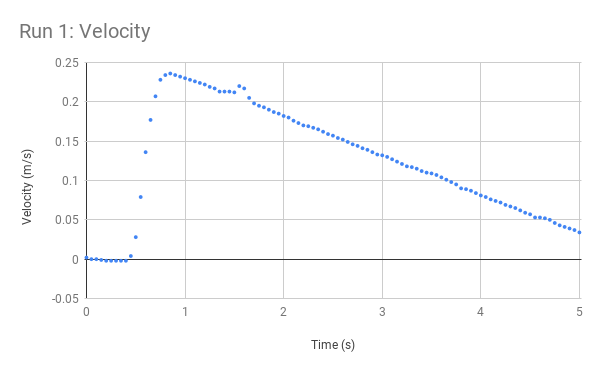
\includegraphics[scale=0.71]{image/03-first-law/Run-1-Velocity.png}
    \caption{Run 1: No friction pad}
    \label{figure:03.run-1}
\end{figure}
\vspace{\stretch{1}}
%%%%%%%%%%%%%%%%%%%%%%%%%%%%%%%%%%%%%%%%%%%%%%%%%%%%%%%%%%%%%%%%%%%%%%%%%%%%%%%%
\begin{figure}[ht]
    \centering
    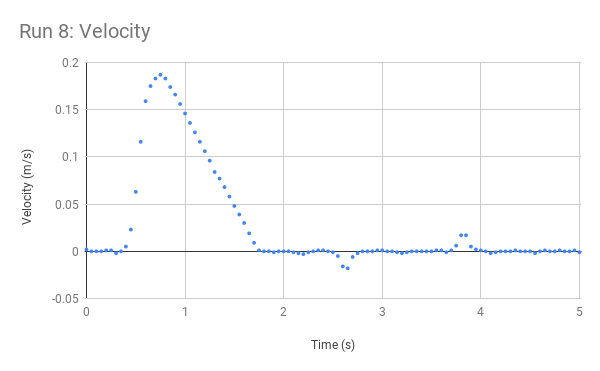
\includegraphics[scale=0.71]{image/03-first-law/Run-8-Velocity.png}
    \caption{Run 8: Friction pad at its lowest}
    \label{figure:03.run-8}
\end{figure}
%%%%%%%%%%%%%%%%%%%%%%%%%%%%%%%%%%%%%%%%%%%%%%%%%%%%%%%%%%%%%%%%%%%%%%%%%%%%%%%%
% Copyright 2018-2019 Melvin Eloy Irizarry-Gelpí
\setcounter{chapter}{3}
\chapter{Newton's Second Law}
%
In this experiment you will check the validity of Newton's second law of motion.
%
\section{Preliminary}
%
The newtonian approach to describing motion involves concepts like mass, acceleration, and forces. \textbf{Newton's second law} relates these three concepts in a mathematical way:
\begin{itemize}
    \item The amount of \textbf{net force} acting on an object is directly proportional to the amount of \textbf{acceleration} of the object. The constant of proportionality is the \textbf{mass} of the object.
\end{itemize}
In equation form:
\begin{equation}
    F_{\text{net}} = m a
    \label{eq:04.Fma}
\end{equation}
One way to check the validity of Newton's second law would be to measure the net force acting on an object, and also the acceleration resulting from this net force, and check whether the data has a linear shape.
%
\section{Experiment}
%
You used an Atwood machine, which is a device involving weights and pulleys. A cart holding a picket fence and a force sensor is attached to a piece of string. The other end of the string has some amount of mass attached to it, that is allowed to hang through a pulley. When the cart is allowed to move, the weight will fall downward and pulled on the string down, and the cart forward. By changing the amount of mass hanging, you can change the amount of net force acting on the cart. You used a photogate to measure the velocity of the cart, and a force sensor to measure the amount of force acting on the cart.
%
\section{Analysis}
%
Here are the steps to follow.
%
\subsection{Calculate the Slope from Velocity and Time}
%
For each run, the photogate gives you distance, velocity and acceleration data, along with gate state, as they change with time. You are only interested in the velocity and time columns. It is okay that for some time values there is no velocity value listed. This just reflects the fact that the velocity data is not really measured but computed from the time data (along with gate state and knowledge of the size of the picket fence). In any case, a chart with velocity in the vertical axis and time in the horizontal axis looks linear. As done many times before, you can include the best-fit line and find the slope and intercept. The slope corresponds to the \textbf{acceleration} experience by the cart. See the second column in Table \ref{table:04.results} for my results.
%
\subsection{Calculate the Time-Averaged Force}
%
For each run, the force sensor gives you the amount of force acting on the cart as time passes. A chart with force in the vertical axis and time in the horizontal axis looks like the amount of force changes over time and thus it is not constant. But a closer look indicates that the values are not changing by a significant amount, and thus this variation is mostly due to random noise. One way to extract a single force value is to calculate the average force over the time period. This is known as the \textbf{time-averaged force}. See the third column in Table \ref{table:04.results} for my results.
%
\subsection{Calculate the 3-Run Averages}
%
It is always a good idea to check for consistency by repeating a measurement. With three runs using the same hanging mass, the value of the slope and the time-averaged force should be consistent. You can average each of these three values and obtain your best experimental estimate for the acceleration of the cart, and the amount of force acting on the cart, given an amount of hanging mass. See Table \ref{table:04.averages} for my results.
%
\subsection{Calculate the Slope from Force and Acceleration}
%
If you used six different values for the hanging mass, then you should have six pairs of 3-run average acceleration (slope), and 3-run time-averaged force. Make a chart with force in the vertical axis and acceleration in the horizontal axis. Add the best-fit linear function and record the slope value. Based on Equation \ref{eq:04.Fma} the slope should correspond to the total mass of the object moving along the track. This mass is the sum of the mass of
\begin{enumerate}
    \item the picket fence,
    \item the force sensor,
    \item and the cart.
\end{enumerate}
Make sure you use a scale to find these values for your experiment. See Table \ref{table:04.masses} for my case.
%
\section{My Data}
%
My data consist of 18 runs:
\begin{itemize}
    \item Runs 1, 2, and 3: 50 g of mass hanging.
    \item Runs 4, 5, and 6: 70 g of mass hanging.
    \item Runs 7, 8, and 9: 80 g of mass hanging.
    \item Runs 10, 11, and 12: 100 g of mass hanging.
    \item Runs 13, 14, and 15: 120 g of mass hanging.
    \item Runs 16, 17, and 18: 150 g of mass hanging.
\end{itemize}
%
\section{Your Data}
%
You should have at least three runs for each of at least six different hanging masses.
%
\newpage
\section{Your Laboratory Report}
%
Your report should include the following:
\begin{enumerate}
    \item One chart with velocity in the vertical axis, and time in the horizontal axis. Include the best-fit line, and display the equation in the legend.
    \item One chart with force in the vertical axis, and time in the horizontal axis.
    \item A table like Table \ref{table:04.results} with slope and time-averaged force for each run.
    \item A table like Table \ref{table:04.averages} with the 3-run averages.
    \item A table like Table \ref{table:04.masses} with the mass values that you measured.
    \item A chart like Figure \ref{figure:04.fma} with force in the vertical axis and acceleration in the horizontal axis. Include the best-fit line and display the equation for it in the legend.
    \item Calculate the percent difference between the slope from your force versus acceleration chart and the expected total mass value.
    \item Do you find that Newton's second law of motion holds true?
\end{enumerate}
You are free to choose which run to use for items 1 and 2.
%
\newpage
\section{Tables}
%
\begin{table}[ht]
    \centering
    \begin{tabular}{|l|r|r|}
        \hline
        Run & Slope (m/s$^{2}$) & Time-Averaged Force (N) \\
        \hline
        1 & 0.67 & 0.426 \\
        2 & 0.66 & 0.426 \\
        3 & 0.62 & 0.431 \\
        \hline
        4 & 0.92 & 0.583 \\
        5 & 0.91 & 0.585 \\
        6 & 0.88 & 0.589 \\
        \hline
        7 & 1.03 & 0.657 \\
        8 & 1.02 & 0.659 \\
        9 & 1.02 & 0.658 \\
        \hline
        10 & 1.27 & 0.800 \\
        11 & 1.25 & 0.797 \\
        12 & 1.26 & 0.796 \\
        \hline
        13 & 1.49 & 0.943 \\
        14 & 1.50 & 0.944 \\
        15 & 1.51 & 0.944 \\
        \hline
        16 & 1.81 & 1.135 \\
        17 & 1.83 & 1.132 \\
        18 & 1.83 & 1.130 \\
        \hline
    \end{tabular}
    \caption{Slope of velocity versus time, and time-averaged force}
    \label{table:04.results}
\end{table}
\vspace{\stretch{1}}
%
\begin{table}[ht]
    \centering
    \begin{tabular}{|l|r|r|}
        \hline
        Runs & Average Slope (m/s$^{2}$) & Average Time-Averaged Force (N) \\
        \hline
        1, 2, and 3 & 0.65 & 0.427 \\
        4, 5, and 6 & 0.90 & 0.586 \\
        7, 8, and 9 & 1.02 & 0.658 \\
        10, 11, and 12 & 1.26 & 0.798 \\
        13, 14, and 15 & 1.50 & 0.944 \\
        16, 17, and 18 & 1.82 & 1.132 \\
        \hline
    \end{tabular}
    \caption{3-Run Averages}
    \label{table:04.averages}
\end{table}
\vspace{\stretch{1}}
%
\begin{table}[ht]
    \centering
    \begin{tabular}{|l|r|}
        \hline
        Name & Value (kg) \\
        \hline
        Mass of picket fence & 0.01298 \\
        Mass of force sensor & 0.08775 \\
        Mass of cart & 0.50149 \\
        \hline
        Total mass & 0.60222 \\
        \hline
    \end{tabular}
    \caption{Mass values}
    \label{table:04.masses}
\end{table}
\vspace{\stretch{1}}
%
\FloatBarrier
\newpage
\section{Figures}
%
\begin{figure}[ht]
    \centering
    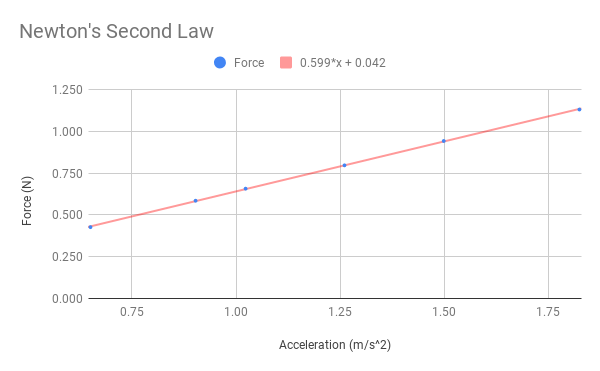
\includegraphics[scale=0.71]{image/04-second-law/newton-2nd-law.png}
    \caption{Force versus Acceleration}
    \label{figure:04.fma}
\end{figure}
% Copyright 2018-2020 Melvin Eloy Irizarry-Gelpí
% \setcounter{chapter}{4}
\chapter{Newton's Third Law}
%
In this experiment you will check the validity of Newton's third law of motion.
%
\section{Preliminary}
%
The \textbf{third law of motion} can be stated as follows:
\begin{itemize}
    \item Whenever A exerts a force $\vec{F}_{AB}$ on B, B exerts a force $\vec{F}_{BA}$ on A.
    \item The \textbf{magnitude} of the forces $\vec{F}_{BA}$ and $\vec{F}_{AB}$ are equal.
    \item The \textbf{direction} of the force $\vec{F}_{BA}$ is the exact opposite of the direction of the force $\vec{F}_{AB}$.
\end{itemize}
In more mathematical terms,
\begin{align}
    \vert \vec{F}_{BA} \vert &= \vert \vec{F}_{AB} \vert & \vec{F}_{BA} &= - \vec{F}_{AB}
\end{align}
One way to test the third law would be to measure the force acting on two bodies and verify that the magnitudes are the same, but that the directions are opposite.

There is a \textbf{common misconception} about the third law. Sometimes, it is stated as
\begin{itemize}
    \item For every action, there is an equal and opposite \textbf{reaction}.
\end{itemize}
This wording leads to an \textbf{incorrect} picture because it introduces an order in time, as in object A first acts on object B, and then, as a reaction, object B acts on object A. This is \textbf{incorrect}. Both forces in Newton's third law appear \textbf{at the same time}. You can check this by measuring the force across time. If the reaction picture were accurate, then you would see a time-delay in one of the forces. Another way to state this is that there is a symmetry between the objects in the sense that there is no breakdown into aggressor and receiver.
%
\section{Experiment}
%
You used two force sensors to measure the amount of force acting on each other. For definiteness, the sensor on the left is called ``Sensor L'', and the sensor on the right is called ``Sensor R'' To check different aspects of the third law, you performed three kinds of experiments:
\begin{itemize}
    \item Sensor L pulls/pushes on sensor R.
    \item Sensor R pulls/pushes on sensor L.
    \item Both sensors pull/push on each other.
\end{itemize}
Furthermore, you tried different attachments on the force sensors:
\begin{itemize}
    \item String (pulling)
    \item Elastic Band (pulling)
    \item Bumpers (pushing)
    \item Magnets (pushing)
\end{itemize}
The force sensors give you force values (in N) over time (in s).
%
\section{Analysis}
%
Here is what to do. For illustration purposes, I will work with the runs using the \textbf{magnets}.
%
\subsection{Plot Both Forces Versus Time}
%
With the force values from each sensor you can make line charts. Figures \ref{figure:05.ff.L}, \ref{figure:05.ff.R}, and \ref{figure:05.ff.B} display the three runs with magnets. As you can see, the three charts are very symmetric about the horizontal axis, supporting the notion that each force sensor measures about the same amount of force at the same amount of time, but with different signs.

Another thing to notice, is that the three charts mentioned above are very similar and without any labels one could not tell if either sensor is doing the pushing, or both. For example, there is nothing special about Figure \ref{figure:05.ff.L} that distinctively indicates that the left sensor is pushing on the right sensor.
%
\subsection{Plot Sum of Forces Versus Time}
%
Besides visually examining the charts with the two force columns, you can calculate and also visualize the \textbf{sum of the two force columns}. Figures \ref{figure:05.sf.L}, \ref{figure:05.sf.R}, and \ref{figure:05.sf.B} display the three runs with magnets. As you can see the sum of the forces takes on very small values with no clear pattern. Indeed, the values are comparable to the starting values before any pushing is done. This indicates that, for practical purposes, the sum of the two forces amounts to noise. That is, the result of adding the two force columns gives a column of force values that are indistinguishable from a noise reading.

Again, all three charts here are very similar, so without labels you could not tell which chart corresponds to which run (i.e. which sensor was doing the pushing).
%
\subsection{Find Time-Averaged Values}
%
In order to summarize each run, you can calculate the time-averaged value of the amount of force acting on each sensor, and also the time-averaged value of the sum of the forces. In Table \ref{table:05.results} you can find my results. As you can see, the magnitude of the values in the second column are very close to the magnitude of the values in the third column. This is consistent with Newton's third law. Also, the values in the fourth column are very small. Although the values in the fourth column are not exactly zero, the values are indistinguishable from noise values. This observation allows me to conclude that the sum of forces averages to a value that could be measured as effectively zero. This is also consistent with Newton's third law.

Another observation from Table \ref{table:05.results} is that there is no clear pattern among the runs associated to a given attachment. That is, from the values alone, you cannot tell which sensor is pushing/pulling.

Yet another observation from Table \ref{table:05.results} is that both pulling cases are consistent, and also both pushing cases are consistent. That is, you cannot tell from the values which run had a string or an elastic band. This is as expected: Newton's third law of motion does not depend on the nature of the force.
%
\section{My Data}
%
Here is a breakdown of my runs:
\begin{enumerate}
    \item String (left pulling)
    \item String (right pulling)
    \item String (both pulling)
    \item String (left pulling)
    \item String (right pulling)
    \item String (both pulling)
    \item Elastic band (left pulling)
    \item Elastic band (right pulling)
    \item Elastic band (both pulling)
    \item Bumpers (left pushing)
    \item Bumpers (right pushing)
    \item Bumpers (both pushing)
    \item Magnets (left pushing)
    \item Magnets (right pushing)
    \item Magnets (both pushing)
\end{enumerate}
I got distracted and accidentally forgot to replace the string with the elastic band, so collected double the amount of data for the string.
%
\section{Your Data}
%
You should have three runs of data for each of the four attachments for the force sensor (total number of runs should be twelve). For each run, you should have a time column, and two force columns. 
%
\newpage
\section{Your Laboratory Report}
%
Your laboratory report should include the following:
\begin{enumerate}
    \item Choose \textbf{one} of the four attachments (string or elastic band or bumpers or magnets). For that choice, make the following \textbf{line charts}:
    \begin{enumerate}
        \item Three charts like Figure \ref{figure:05.ff.L} (one chart for each of the three runs) with force in the vertical axis and time in the horizontal axis, showing \textbf{both} force columns.
        \item Three charts like Figure \ref{figure:05.sf.L} (one chart for each of the three runs) with force in the vertical axis and time in the horizontal axis, showing the \textbf{sum of forces}.
    \end{enumerate}
    \item A table like Table \ref{table:05.results} with the time-averaged values for the force on L, force on R, and sum of forces, for \textbf{all twelve} runs.
\end{enumerate}
You should also include answers to the following questions:
\begin{enumerate}
    \item Looking at your table of time-averaged values (e.g. \ref{table:05.results}), is there a clear pattern that allows you to distinguish runs by the kind of attachment used?
    \item Looking at your table of time-averaged values (e.g. \ref{table:05.results}), is there a clear pattern that allows you to tell from the values which sensor was pushing/pulling?
    \item Besides the sign in the force values, is there are anyway of telling the pushing forces apart from the pulling forces?
    \item Imagine Figures \ref{figure:05.ff.L}, \ref{figure:05.ff.R}, and \ref{figure:05.ff.B} had no labels. Could you tell from looking at a chart whether the left sensor was pushing or the right sensor was pushing or both were pushing?
    \item Imagine Figures \ref{figure:05.sf.L}, \ref{figure:05.sf.R}, and \ref{figure:05.sf.B} had no labels. Could you tell from looking at a chart whether the left sensor was pushing or the right sensor was pushing or both were pushing?
    \item Do you find that Newton's third law holds? Remember that small force values could be indistinguishable from noise.
\end{enumerate}
%
\newpage
\section{Example Tables}
%
\begin{table}[ht]
    \centering
    \begin{tabular}{l|r|r|r|c}
        \textbf{Run} & \textbf{Force on L} (N) & \textbf{Force on R} (N) & \textbf{Sum of Forces} (N) & \textbf{Attachment} \\
        \hline
        1 & 3.980 & \textminus 4.053 & \textminus 0.073 & \\
        2 & 1.499 & \textminus 1.571 & \textminus 0.071 & String \\
        3 & 1.948 & \textminus 1.976 & \textminus 0.028 & \\
        \hline
        4 & 2.167 & \textminus 2.225 & \textminus 0.058 & \\
        5 & 2.248 & \textminus 2.335 & \textminus 0.086 & String \\
        6 & 3.653 & \textminus 3.771 & \textminus 0.119 & \\
        \hline
        7 & 1.673 & \textminus 1.772 & \textminus 0.098 & \\
        8 & 2.002 & \textminus 2.049 & \textminus 0.047 & Elastic Band \\
        9 & 2.362 & \textminus 2.420 & \textminus 0.059 & \\
        \hline
        10 & \textminus 3.913 & 3.945 & 0.033 & \\
        11 & \textminus 3.670 & 3.692 & 0.022 & Bumpers \\
        12 & \textminus 4.638 & 4.627 & \textminus 0.012 & \\
        \hline
        13 & \textminus 2.121 & 2.089 & \textminus 0.032 & \\
        14 & \textminus 3.008 & 2.968 & \textminus 0.040 & Magnets \\
        15 & \textminus 4.064 & 4.025 & \textminus 0.039 & \\
        \hline
    \end{tabular}
    \caption{Time-Averaged Values.}
    \label{table:05.results}
\end{table}
%
\FloatBarrier
\newpage
\section{Example Charts}
%
\begin{figure}[ht]
    \centering
    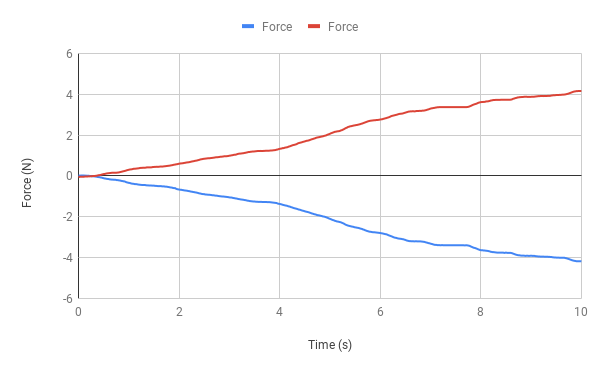
\includegraphics[scale=0.71]{image/05-third-law/Run-13-Both.png}
    \caption{Both Forces versus Time; Left Pushing}
    \label{figure:05.ff.L}
\end{figure}
%
\begin{figure}[ht]
    \centering
    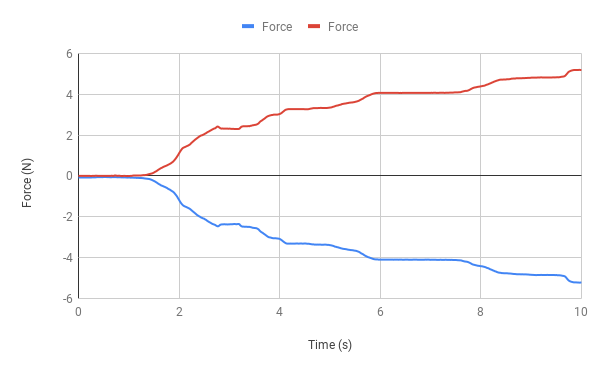
\includegraphics[scale=0.71]{image/05-third-law/Run-14-Both.png}
    \caption{Both Forces versus Time; Right Pushing}
    \label{figure:05.ff.R}
\end{figure}
%
\begin{figure}[ht]
    \centering
    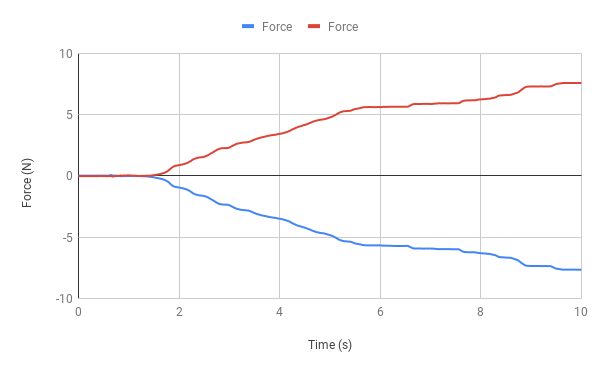
\includegraphics[scale=0.71]{image/05-third-law/Run-15-Both.png}
    \caption{Both Forces versus Time; Both Pushing}
    \label{figure:05.ff.B}
\end{figure}
%
\begin{figure}[ht]
    \centering
    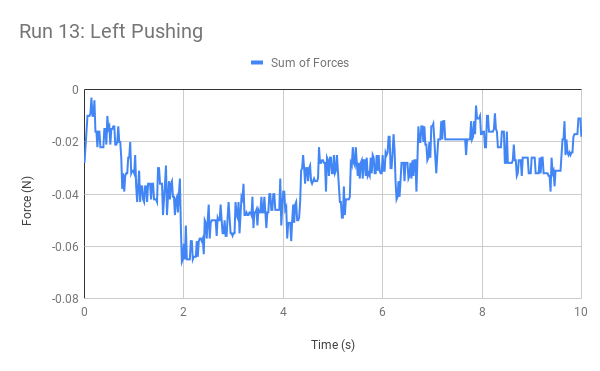
\includegraphics[scale=0.71]{image/05-third-law/Run-13-Left-Pushing.png}
    \caption{Sum of Forces versus Time; Left Pushing}
    \label{figure:05.sf.L}
\end{figure}
%
\begin{figure}[ht]
    \centering
    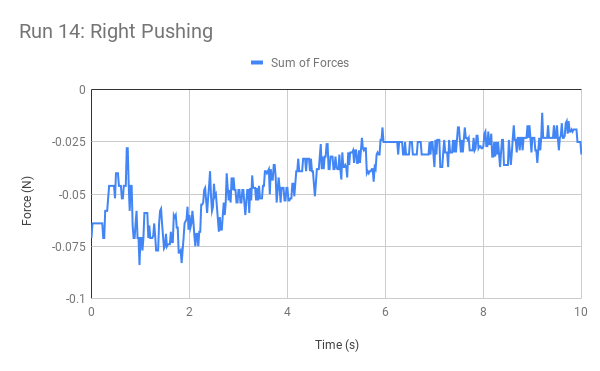
\includegraphics[scale=0.71]{image/05-third-law/Run-14-Right-Pushing.png}
    \caption{Sum of Forces versus Time; Right Pushing}
    \label{figure:05.sf.R}
\end{figure}
%
\begin{figure}[ht]
    \centering
    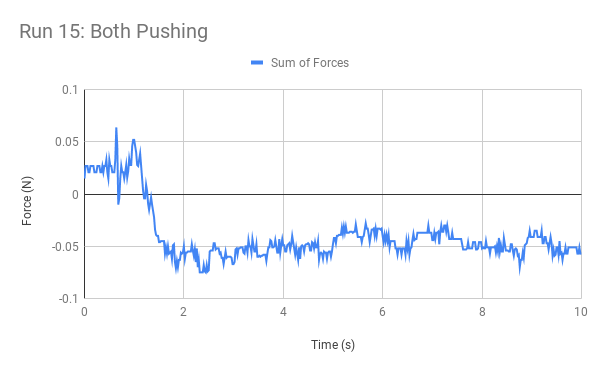
\includegraphics[scale=0.71]{image/05-third-law/Run-15-Both-Pushing.png}
    \caption{Sum of Forces versus Time; Both Pushing}
    \label{figure:05.sf.B}
\end{figure}
%
\part{Energy}
% Copyright 2018-2020 Melvin Eloy Irizarry-Gelpí
% Laboratory 6
\setcounter{chapter}{5}
\chapter{Kinetic and Elastic Potential Energy}
%
In this experiment you will check that kinetic energy depends on speed in a quadratic way.
%
\section{Preliminary}
%
Energy is a fundamental concept in physics. Unlike force, which is a vector quantity, energy has no intrinsic direction. The \textbf{SI unit} for energy is the joule (J). One joule of energy is equivalent to 1 newton-meter:
\begin{equation}
    1 \ \text{J} = 1 \ \text{N {\textperiodcentered} m}
\end{equation}
There are many forms of energy. \textbf{Kinetic energy} is the energy associated to being in a state of \textbf{motion}. Not surprisingly, the amount of kinetic energy $K$ of an object depends on the amount of mass $m$ and the amount of speed $v$ (not velocity $\mathbf{v}$). As you will check, the amount of kinetic energy is quadratic in speed:
\begin{equation}
    K = \frac{1}{2} m v^{2}
\end{equation}
Note that kinetic energy cannot be negative, because mass and square speed are always non-negative. If the speed is zero, then you have zero kinetic energy. That is, an object at rest has zero amount of kinetic energy.

A simple direct experiment to test that kinetic energy depends on speed as stated above would involve measuring the speed $v$ and the energy $K$ of a moving object, and checking that the chart with speed and kinetic energy is quadratic. However, we do not have a sensor that measures kinetic energy directly.

When you compress or stretch a spring, you are storing a form of energy known as \textbf{elastic potential energy}. The amount of elastic potential energy $U$ stored in a spring with spring constant $k$ that is compressed/stretched a distance from equilibrium $x$ is given by
\begin{equation}
    U = \frac{1}{2} k x^{2}
\end{equation}
Note that, like kinetic energy, elastic potential energy cannot be negative, since $k$ and $x^{2}$ are non-negative. If the distance from equilibrium is zero, then you have zero elastic potential energy. That is, when the spring is in its relaxed shape, it stores zero amount of elastic potential energy. The mathematical form of $U$ is very similar to the mathematical form of $K$.
%
\subsection{The spring constant}
%
If the value of the spring constant $k$ is not known, you can use Hooke's law to find it:
\begin{equation}
    F = -kx
\end{equation}
Here $F$ is the amount of force applied on the spring when stretched/compressed a distance $x$. Since the amount of force is directly proportional to the distance, the spring constant can be found as the slope in a force versus distance chart. Note that in SI units, the spring constant has units of N/m.
%
\subsection{Mechanical energy}
%
Elastic potential energy is an example of energy that can be stored over time and used later. Such kinds of energy are known as potential energy. Another important form of energy is \textbf{mechanical energy}, which is just the sum of kinetic energy and any form of potential energy available. The symbol for mechanical energy is $E$:
\begin{equation}
    E = K + U
\end{equation}
Sometimes, the value of mechanical energy is constant over time and does not change during the motion of an object. This is known as conservation of mechanical energy.
%
\section{Experiment}
%
You have a cart with a picket fence. The cart can move along a flat track. You can use a photogate to measure the speed of the cart at a given point along the track. You have a spring loop attached to one end of the track. When you push the cart against the spring loop, you compress the spring loop, and you do \textbf{work} (another form of energy). This work is stored on the spring as elastic potential energy. While holding the cart against the spring, the cart is not moving, so the speed of the cart is zero. Thus, at this point in time, the cart has zero kinetic energy. As stated above, the amount of elastic potential energy depends on how much the spring is compressed. At this point in time the mechanical energy, the sum of the kinetic and elastic potential energy, is just purely elastic:
\begin{equation}
    E_{1} = K + U = \frac{1}{2} m v^{2} + \frac{1}{2} k x^{2} = \frac{1}{2} k x^{2}
\end{equation}
Then you release the cart. The spring now expands to its equilibrium shape ($x = 0$). As the spring expands, it pushes the cart forward, transferring the elastic potential energy to the cart. The cart is now moving, so it has kinetic energy. This energy came from the elastic potential energy of the spring. At this moment, the mechanical energy is just purely kinetic:
\begin{equation}
    E_{2} = K + U = \frac{1}{2} m v^{2} + \frac{1}{2} k x^{2} = \frac{1}{2} m v^{2}
\end{equation}
One of the most important properties of energy is that it is \textbf{conserved}. Specifically, energy cannot be created from nothing, or destroyed into nothing: you can only convert one form of energy into another. Furthermore, in some cases, like this experiment with the cart and the spring loop, the amount of mechanical energy does not change with time. That means that the value of the mechanical energy when the spring is compressed and there is no motion, $E_{1}$, should be equal to the value of the mechanical energy when the spring is not compressed and there is motion, $E_{2}$. That is,
\begin{equation}
    E_{1} = E_{2}
\end{equation}
This means that
\begin{equation}
    \frac{1}{2} m v^{2} = \frac{1}{2} k x^{2}
\end{equation}
Simplifying a bit, you get a relation between the square of speed, and the square of the distance from equilibrium:
\begin{equation}
    v^{2} = \left( \frac{k}{m} \right) x^{2}
\end{equation}
You can verify this relation by measuring the speed of a cart just after being launched by a spring from a certain amount of distance from equilibrium.

For future reference, you can introduce the following quantity
\begin{equation}
    \omega^{2} = \frac{k}{m}
\end{equation}
Here $\omega$, the lowercase Greek letter omega, is known as the \textbf{angular frequency}. The SI unit for angular frequency is radian per second. A radian is a way of measuring the size of an angle. For practical purposes, a radian unit is equivalent to a plain number with no units. In terms of $\omega$, the above relation between $v^{2}$ and $x^{2}$ is given by
\begin{equation}
    v^{2} = \omega^{2} x^{2}
\end{equation}
Thus, a chart with $v^{2}$ in the vertical axis, and $x^{2}$ in the horizontal axis should have a linear shape with slope being close to $\omega^{2}$.
%
\section{Analysis}
%
Here are the steps to follow:
%
\subsection{Measure the position of the equilibrium shape}
%
You can use the marking on the track to measure the position of the cart when the cart is just touching the spring loop and the spring loop is not compressed. This position will be called $d_{0}$ and will be used next to find the distance from equilibrium.
%
\subsection{Calculate the distance from equilibrium}
%
You recorded the launch position $d$ of the cart. Together with the equilibrium position $d_{0}$, you can calculate the distance from equilibrium $x$:
\begin{equation}
    x = d_{0} - d
\end{equation}
This definition of $x$ guarantees that $x$ will be positive.
%
\subsection{Find the 3-run average speed}
%
It is good practice to, for a given launch position, repeat a launch and record at least three consistent values of the speed of the cart. You can find the 3-run average speed and use that as your best estimate for the speed of the cart when being launched from that particular position.
%
\subsection{Visualize velocity versus distance}
%
You can make a chart with speed $v$ in the vertical axis and distance from equilibrium $x$ in the horizontal axis. According to the expected model, the chart should have a linear shape and the slope should be related to $\omega$. However, since you do not know the value of the spring constant $k$, you cannot determine the expected value of $\omega$. Indeed, you can use this experiment to measure $\omega$.

In my case, Figure \ref{figure:06.v} shows the relation between $v$ and $x$. As you can see, the relation is linear. The chart includes the best-fit line.
%
\subsection{Visualize squared velocity versus squared distance}
%
The relation between $v$ and $x$ from energy conservation involves the square quantities. It does not hurt to check the linear quantities, but a real test should involve the squares. In new spreadsheet columns you can calculate the square speed and the square of the distance from equilibrium. Then you can make a chart with $v^{2}$ in the vertical axis and $x^{2}$ in the horizontal axis. The expectation is that this chart should also have a linear shape, with a very small intercept, and a slope related to $\omega^{2}$.

In my case, Figure \ref{figure:06.v.2} shows the relation between $v^{2}$ and $x^{2}$. The data also has a linear shape.
%
\subsection{Estimate the value of the spring constant}
%
You can use a digital scale to find the value of the mass of the cart, and the mass of the picket fence. The sum of these masses, gives you the total mass of the object that the spring pushes away. In Table \ref{table:06.mass} you can find the values for my case.

The slope in Figure \ref{figure:06.v.2} provides an estimate for $\omega^{2}$:
\begin{equation}
    \omega^{2} \approx 62.3 \ \text{rad\textsuperscript{2}/s\textsuperscript{2}}
\end{equation}
Using the definition of $\omega^{2}$ to solve for $k$ gives
\begin{equation}
    k = \omega^{2} m \approx \left( 62.3 \ \text{rad\textsuperscript{2}/s\textsuperscript{2}} \right) \left( 0.5218 \ \text{kg} \right) = 31.508 \ \text{N/m}
\end{equation}
The spring constant for the spring loop will be slightly different for each spring, but your result should be close to 30 N/m.
%
\section{My Data}
%
My raw data for launch position and speed is in Table \ref{table:06.data}. The first column has the position of launch. The second column has the corresponding distance from equilibrium. The third, fourth, and fifth columns have the speed of the cart measured by the photogate. The last column has the 3-run average speed. I considered seven compressed distances, plus the first row that corresponds to an uncompressed spring.
%
\section{Your Data}
%
Your data should be very similar to mine, but the actual launch positions might be different due to the varying shapes of the spring loops. You should have a total of eight data points.
%
% \newpage
% \section{Your Laboratory Report}
% %
% Your lab report should include the following:
% \begin{enumerate}
%     \item A table like Table \ref{table:06.mass} with the mass values you measured.
%     \item A table like Table \ref{table:06.data} with the positions you used for launching the cart, the corresponding distance from equilibrium, the speed you measured, and the 3-run average speed.
%     \item A chart with $v^{2}$ in the vertical axis, and $x^{2}$ in the horizontal axis. Include the best fit line, along with the equation.
%     \item Use the slope value to estimate $\omega^{2}$. Then use this estimate of $\omega^{2}$ and the total mass of the object to estimate the value of the spring constant $k$ for the spring loop.
% \end{enumerate}
%
\newpage
\section{Your Laboratory Worksheet}
%
Please print your work before coming to class.
%
\paragraph{Part 1: Spring constant}
%
\begin{enumerate}
    \item Provide a \textbf{scatter chart} with force in the vertical axis, and distance from equilibrium in the horizontal axis. If the data has a linear shape, include a best-fit line and display its equation.
    \item Use Hooke's law to determine observed value of the spring constant for the loop you used.
\end{enumerate}
%
\paragraph{Part 2: Angular frequency}
%
\begin{enumerate}
    \item For each distance from equilibrium, you collected three runs with velocity data. Provide a \textbf{table} with
    \begin{itemize}
        \item the distance from equilibrium $x$
        \item the 3-run average velocity $v$
    \end{itemize}
    You should have 8 rows with data.
    \item Provide a scatter chart with $v^{2}$ in the vertical axis, and $x^{2}$ in the horizontal axis. If the data has a linear shape, include a best-fit line and display its equation.
    \item Determine the observed value of the squared angular frequency $\omega^{2}$ for the mass and loop you used.
\end{enumerate}
%
\paragraph{Part 3: Results}
%
\begin{enumerate}
    \item Provide a \textbf{table} with
    \begin{itemize}
        \item the mass of the cart you used
        \item the mass of the picket fence you used
        \item the total mass
    \end{itemize}
    \item Use the total mass you measured, and the value of the squared angular frequency you obtained above, to obtain another estimate of the spring constant for the loop. How do both values compare?
\end{enumerate}
%
\newpage
\section{Table Templates}
%
\begin{table}[ht!]
    \begin{center}
        \begin{tabular}{l | l | l | l | l | l}
            \textbf{Label} & $x$ (cm) & $v_{1}$ (m/s) & $v_{2}$ (m/s) & $v_{3}$ (m/s) & 3-run average $v$ (m/s) \\
            \hline
            1 & & & & & \\
            2 & & & & & \\
            3 & & & & & \\
            4 & & & & & \\
            5 & & & & & \\
            6 & & & & & \\
            7 & & & & & \\
            8 & & & & & \\
            \hline
        \end{tabular}
    \end{center}
    \caption{Sample Table 1}
\end{table}
%
\begin{table}[ht!]
    \begin{center}
        \begin{tabular}{l | l}
            & \textbf{Mass} (kg) \\
            \hline
            Cart & \\
            Picket fence & \\
            \hline
            Total & \\
            \hline
        \end{tabular}
    \end{center}
    \caption{Sample Table 2}
\end{table}
%
\newpage
\section{Example Tables}
%
\begin{table}[ht]
    \centering
    \begin{tabular}{l|r}
        \textbf{Name} & \textbf{Value} (kg) \\
        \hline
        Mass of cart & 0.5088 \\
        Mass of picket fence & 0.013 \\
        \hline
        Total mass & 0.5218 \\
        \hline
    \end{tabular}
    \caption{Mass measurements}
    \label{table:06.mass}
\end{table}
%
\begin{table}[ht]
    \centering
    \begin{tabular}{l|r|r|r|r|r}
        $d$ (cm) & $x$ (cm) & $v_{1}$ (m/s) & $v_{2}$ (m/s) & $v_{3}$ (m/s) & Average $v$ (m/s) \\
        \hline
        11 & 0 & 0 & 0 & 0 & 0 \\
        10 & 1 & 0.079 & 0.081 & 0.077 & 0.079 \\
        9.5 & 1.5 & 0.122 & 0.124 & 0.125 & 0.124 \\
        9 & 2 & 0.162 & 0.164 & 0.151 & 0.159 \\
        8.5 & 2.5 & 0.197 & 0.211 & 0.199 & 0.202 \\
        8 & 3 & 0.236 & 0.235 & 0.238 & 0.236 \\
        7.5 & 3.5 & 0.274 & 0.274 & 0.279 & 0.276 \\
        7 & 4 & 0.317 & 0.312 & 0.322 & 0.317 \\
        \hline
    \end{tabular}
    \caption{Raw Data}
    \label{table:06.data}
\end{table}
%
\newpage
\section{Example Charts}
%
\begin{figure}[ht]
    \centering
    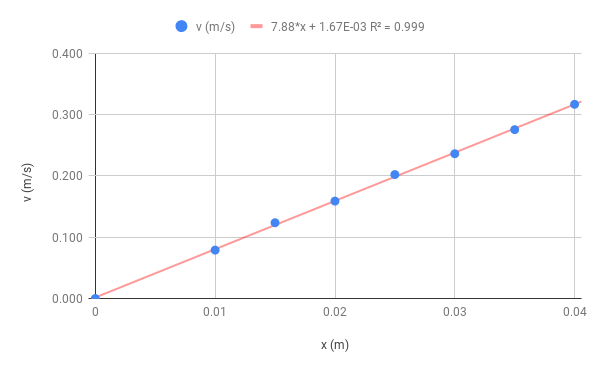
\includegraphics[scale=0.71]{image/06-kinetic/v.png}
    \caption{Velocity versus distance from equilibrium}
    \label{figure:06.v}
\end{figure}
%
\begin{figure}[ht]
    \centering
    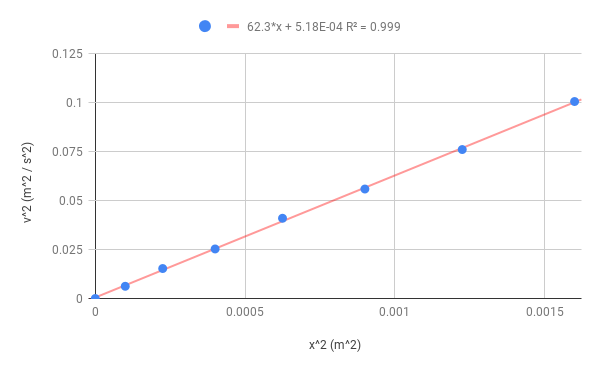
\includegraphics[scale=0.71]{image/06-kinetic/v2.png}
    \caption{Square of Velocity versus square of distance from equilibrium}
    \label{figure:06.v.2}
\end{figure}
%
% Copyright 2018-2020 Melvin Eloy Irizarry-Gelpí
% \setcounter{chapter}{6}
\chapter{Kinetic and Gravitational Energy}
%
In this experiment you will study the dependance of gravitational energy on height.
%
\section{Preliminary}
%
In the previous experiment, you encountered \textbf{kinetic} energy (the energy associated to being in motion), \textbf{elastic} energy (the potential energy associated to deforming a spring), and \textbf{mechanic} energy (the sum of kinetic and potential energy).

The amount of \textbf{kinetic} energy $K$ depends on the amount of mass $m$ and speed $v$:
\begin{equation}
    K = \frac{1}{2} m v^{2}
\end{equation}
Note that kinetic energy changes if the speed of the object changes.

Another form of energy is \textbf{gravitational} energy (a form of \textbf{potential} energy), which is associated to being in a region with a gravitational field. The amount of gravitational energy $U_{g}$ depends on the amount of mass $m$, the amount of gravitational acceleration $g$, and the amount of height $h$ measured from a fixed reference point:
\begin{equation}
    U_{g} = m g h
\end{equation}
Note that the gravitational energy changes if the height of the object changes. Recall that, on the surface of Earth, $g = 9.80$ m/s$^{2}$.

Finally, you have \textbf{mechanic} energy. The amount of mechanic energy $E$ is the sum of kinetic energy $K$ and potential energy. For the previous experiment, the potential energy was only elastic energy because you had a spring and the object moved along a horizontal track. In the case when the potential energy is only gravitational in nature, the mechanic energy is
\begin{equation}
    E = K + U_{g}
\end{equation}
Energy cannot be created nor destroyed; it can only be transformed into other forms of energy. In a closed system, where energy is not added nor removed by an external source, mechanic energy $E$ is \textbf{constant in time}.

If the object only moves and feels gravity, then the mechanic energy $E$ is given by
\begin{equation}
    E = \frac{1}{2} m v^{2} + m g h
\end{equation}
Solving for $v^{2}$ you get
\begin{equation}
    v^{2} = \left( - 2 g \right) h + \left( \frac{2 E}{m} \right)
    \label{eq.07.vv}
\end{equation}
This relation predicts that $v^{2}$ is a \textbf{linear function} of $h$ with the \textbf{slope} being $-2g$ and the \textbf{intercept} being $2 E / m$. That is, the data in a $v^{2}$ versus $h$ chart should have a \textbf{linear shape}.
%
\section{Experiment}
%
In order to study a system where there is gravitational energy, and also that the gravitational energy changes with time, you used an object moving along an inclined track. With a motion sensor, you recorded the \textbf{position} $d$ and \textbf{velocity} $v$ along the incline as they changed with time. You also recorded some height measurements to determine the sine of the angle of inclination of the inclined track. Also, you recorded the mass $m$ of the cart.
%
\section{Analysis}
%
You would like to test two predictions:
\begin{enumerate}
    \item Mechanic energy does not change with time.
    \item There is a linear relation between $v^{2}$ and $h$ given by Equation \ref{eq.07.vv}.
\end{enumerate}
To test the first prediction, you need to compute the mechanic energy with the data that you collected. To test the second prediction, you need to make a graph with $v^{2}$ in the vertical axis and $h$ in the horizontal axis. Here are some steps to complete the analysis.
%
\subsection{Truncate the Data}
%
Before you can do anything with the data from the experiment, you need to isolated the part of the data where the motion along the incline is happening. In order to know where to cut the data, it is best to make a scatter chart with \textbf{velocity} in the vertical axis and \textbf{time} in the horizontal axis. There are three kinds of truncation:
\begin{enumerate}
    \item Upward motion only: find the time just after the velocity values begin the diagonal downward trend, and the time when the velocity is close to zero
    \item Downward motion only: find the time when the velocity is close to zero, and the time just before the velocity ends the diagonal downward trend
    \item Upward and downward motion: find the time just after the velocity values begin the diagonal downward trend, and the time just before the downward trend ends
\end{enumerate}
Once you know the initial time and the final time of the motion, just delete the data outside of this time interval.

However, for convenience, you might want to truncate the data as a last step, after calculating everything for one full run, and duplicating the sheet for the other runs.
%
\subsection{Kinetic Energy}
%
Here are the steps to follow to calculate the kinetic energy at each moment in time.
%
\subsubsection{Calculate the Squared Velocity}
%
In a separate column, you should calculate the squared velocity using the values in the velocity column.
%
\subsubsection{Calculate the Kinetic Energy}
%
In a separate column, you should compute the value of the kinetic energy using the values in the squared velocity column. If $v$ is a velocity value, then the corresponding kinetic energy is given by
\begin{equation}
    K = \frac{1}{2} m v^{2}
\end{equation}
For the mass, you should use the value of the mass of the cart that you measured with the electronic scale. See Table \ref{table:07.mass} for my case.
%
\subsection{Gravitational Energy}
%
Here are the steps to follow to calculate the gravitational energy at each moment in time.
%
\subsubsection{Calculate the Sine of the Angle of Inclination}
%
You measured the heights of four positions along the incline. Table \ref{table:07.x} has the position values along the track and Tables \ref{table:07.h.1} and Table \ref{table:07.h.2} have the height values. The value of the sine can be found by calculating a ratio of differences. Table \ref{table:07.sine.1} and Table \ref{table:07.sine.2} have three sine calculations for both one-box and two-box inclined tracks.
%
\subsubsection{Calculate Height}
%
In a separate column, you should compute the value of the height at the incline using the values in the position column and the sine. If $d$ is a position value, then the corresponding height is given by
\begin{equation}
    h = d \sin(\theta)
\end{equation}
For sine, use the average of the three sine values you found.
%
\subsubsection{Calculate Gravitational Energy}
%
In a separate column, you should compute the value of the gravitational energy using the values in the height column. If $h$ is a height value, then the corresponding gravitational energy is given by
\begin{equation}
    U_{g} = m g h
\end{equation}
For $g$, use the accepted value of 9.80 m/s$^{2}$.
%
\subsection{Mechanic Energy}
%
Here are the steps to follow to find the mechanic energy.
%
\subsubsection{Calculate the Mechanic Energy}
%
In a separate column, you should compute the value of the mechanic energy using the values in the kinetic and gravitational energy columns. If $K$ is a value in the kinetic energy column, and $U_{g}$ is a value in the gravitational energy column, then the mechanic energy is given by
\begin{equation}
    E = K + U_{g}
\end{equation}
Make sure that you add values that are evaluated at the same time.
%
\subsubsection{Calculate the Time-Average Mechanic Energy}
%
Once you have a column with the mechanic energy values over time, you can calculate the average value of that column and find the \textbf{time-average value of mechanic energy}.
%
\subsection{Visualize Mechanic Energy versus Time}
%
One of the goals of this experiment is to verify that \textbf{mechanic energy is constant in time}. To check this, you can make a scatter chart with time in the horizontal axis and mechanic energy in the vertical axis.

In principle, you should see that the values of mechanic energy do not change with time. In practice, we see that in general the mechanic energy decreases as time passes. This is actually true, since in this experiment you could not completely remove friction and this force leads to \textbf{a loss of energy} to the environment. However, the amount of change in energy over time is very small, so effectively (and approximately) mechanic energy is almost constant.
%
\subsection{Visualize Squared Velocity versus Height}
%
The other goal of this experiment was to verify the linear relation suggested by Equation \ref{eq.07.vv} between $v^{2}$ and $h$ due to conservation of energy. Since the relation is a linear function, the data points should arrange themselves to form a linear shape.

If the data were perfect, then the \textbf{slope} of this linear fit should be given by
\begin{equation} \label{eq.07.slope}
    \text{slope} = -2g = -19.6 \text{ m/s}^{2}
\end{equation}
and the \textbf{intercept} would be related to the amount of mechanic energy via
\begin{equation}
    \text{intercept} = \frac{2 E}{m}
\end{equation}
The slope is negative, so you should see a diagonal line that is downward as height increases. From the intercept you can get a value for mechanic energy that should be close to what you found in the mechanic energy column:
\begin{equation} \label{eq.07.intercept}
    E = \frac{m \times \text{ intercept}}{2}
\end{equation}
You can also compare this value with the time-average value of the mechanic energy.
%
\section{My Data}
%
I collected six runs of data:
\begin{itemize}
    \item Runs 1, 2, and 3: one box of height
    \item Runs 4, 5, and 6: two boxes of height
\end{itemize}
Here are the truncations I used on the spreadsheet:
\begin{itemize}
    \item Run 1 and 4: Upward motion only
    \item Run 2 and 5: Downward motion only
    \item Run 3 and 6: Upward and downward motion
\end{itemize}
As you can see from Figure \ref{figure:07.v2.1} Figure \ref{figure:07.v2.2} and Figure \ref{figure:07.v2.3} the relation between $v^{2}$ and $h$ was found to be very linear. From the best fit line you can find the slope and the intercept. From the intercept, you can use Equation \ref{eq.07.intercept} to find an estimate of the mechanic energy. You can compare this estimate to the time-average value of mechanic energy. Table \ref{table.07.results} summarizes my results.

Although the mechanic energy was found to not be constant in time, as you can see from Figure \ref{figure.07.run.4.e}, Figure \ref{figure.07.run.5.e}, and Figure \ref{figure.07.run.6.e}, the change in energy is very small. Another important feature is that the mechanic energy is almost always getting slightly smaller. This can be explained as due to friction doing a negative amount of work that leads to a loss of mechanic energy.
%
\section{Your Data}
%
You should have six runs of data:
\begin{itemize}
    \item Three runs with one box of height.
    \item Three runs with two boxes of height.
\end{itemize}
Each run should consist of the cart moving upward first, and then downward before being stopped.
%
\newpage
\section{Your Laboratory Report}
%
Your lab report should include the following:
\begin{itemize}
    \item Tables where you show the three estimates of the sine function for both heights, as well as the average (see Table \ref{table:07.sine.1} and Table \ref{table:07.sine.2})
    \item A table with your results for the slope, the time-average value of $E$, and the estimate of $E$ from the intercept, similar to Table \ref{table.07.results}.
    \item One scatter chart with $v^{2}$ in the vertical axis and $h$ in the horizontal axis for \textbf{upward motion} only (see Figure \ref{figure:07.v2.1}). Include the best-fit line.
    \item One scatter chart with $v^{2}$ in the vertical axis and $h$ in the horizontal axis for \textbf{downward motion} only (see Figure \ref{figure:07.v2.2}). Include the best-fit line.
    \item One scatter chart with $v^{2}$ in the vertical axis and $h$ in the horizontal axis for \textbf{both upward and downward motion} (see Figure \ref{figure:07.v2.3}). Include the best-fit line.
    \item One scatter chart with mechanic energy in the vertical axis and time in the horizontal axis for \textbf{upward motion} only (see Figure \ref{figure.07.run.4.e}).
    \item One scatter chart with mechanic energy in the vertical axis and time in the horizontal axis for \textbf{downward motion} only (see Figure \ref{figure.07.run.5.e}).
    \item One scatter chart with mechanic energy in the vertical axis and time in the horizontal axis for \textbf{both upward and downward motion} (see Figure \ref{figure.07.run.6.e}).
\end{itemize}
You should also answer the following questions:
\begin{enumerate}
    \item Are your results for the slope consistent for the three motions considered (upward only, downward only, both upward and downward)?
    \item Did you find mechanic energy to be approximately constant? Or did it changed by a large amount?
    \item If mechanic energy was not found to be constant, did it mostly decrease?
\end{enumerate}
%
\FloatBarrier
\newpage
\section{Tables}
%
\begin{table}[ht]
    \centering
    \begin{tabular}{|l|r|}
        \hline
        Name & Value (cm) \\
        \hline
        $x_{1}$ & 25 \\
        $x_{2}$ & 50 \\
        $x_{3}$ & 75 \\
        $x_{4}$ & 100 \\
        \hline
    \end{tabular}
    \caption{Position values for both one-box and two-box heights}
    \label{table:07.x}
\end{table}
%
\begin{table}[ht]
    \centering
    \begin{tabular}{|l|r|}
        \hline
        Name & Value (cm) \\
        \hline
        $h_{1}$ & 4.3 \\
        $h_{2}$ & 6.1 \\
        $h_{3}$ & 8 \\
        $h_{4}$ & 10 \\
        \hline
    \end{tabular}
    \caption{Height values for one-box height}
    \label{table:07.h.1}
\end{table}
%
\begin{table}[ht]
    \centering
    \begin{tabular}{|l|r|}
        \hline
        Name & Value (cm) \\
        \hline
        $h_{1}$ & 5.2 \\
        $h_{2}$ & 8.4 \\
        $h_{3}$ & 11.7 \\
        $h_{4}$ & 15 \\
        \hline
    \end{tabular}
    \caption{Height values for two-box height}
    \label{table:07.h.2}
\end{table}
%
\begin{table}[ht]
    \centering
    \begin{tabular}{|l|r|}
        \hline
        Name & Value (no units) \\
        \hline
        $\left( h_{2} - h_{1} \right) / \left( x_{2} - x_{1} \right)$ & 0.072 \\
        $\left( h_{3} - h_{2} \right) / \left( x_{3} - x_{2} \right)$ & 0.076 \\
        $\left( h_{4} - h_{3} \right) / \left( x_{4} - x_{3} \right)$ & 0.080 \\
        \hline
        Average Sine & 0.076 \\
        \hline
    \end{tabular}
    \caption{Sine values for one-box height}
    \label{table:07.sine.1}
\end{table}
%
\begin{table}[ht]
    \centering
    \begin{tabular}{|l|r|}
        \hline
        Name & Value (no units) \\
        \hline
        $\left( h_{2} - h_{1} \right) / \left( x_{2} - x_{1} \right)$ & 0.128 \\
        $\left( h_{3} - h_{2} \right) / \left( x_{3} - x_{2} \right)$ & 0.132 \\
        $\left( h_{4} - h_{3} \right) / \left( x_{4} - x_{3} \right)$ & 0.132 \\
        \hline
        Average Sine & 0.131 \\
        \hline
    \end{tabular}
    \caption{Sine values for two-box height}
    \label{table:07.sine.2}
\end{table}
%
\begin{table}[ht]
    \centering
    \begin{tabular}{|l|r|}
        \hline
        Name & Value (kg) \\
        \hline
        Mass of cart & 0.5087 \\
        \hline
    \end{tabular}
    \caption{Mass measurements}
    \label{table:07.mass}
\end{table}
%
\begin{table}[ht]
    \centering
    \begin{tabular}{|l|r|r|r|}
        \hline
        Run & Slope (m/s$^{2}$) & $E$ from Intercept (J) & Time-Average $E$ (J) \\
        \hline
        1 & \textminus 21.47 & 0.3157 & 0.2939 \\
        2 & \textminus 16.84 & 0.2459 & 0.2788 \\
        3 & \textminus 18.98 & 0.3065 & 0.3143 \\
        4 & \textminus 20.75 & 0.5010 & 0.4779 \\
        5 & \textminus 17.62 & 0.4318 & 0.4689 \\
        6 & \textminus 18.97 & 0.4979 & 0.5109 \\
        \hline
    \end{tabular}
    \caption{Summary of results}
    \label{table.07.results}
\end{table}
%
\FloatBarrier
\newpage
\section{Figures}
%
\begin{figure}[ht]
    \centering
    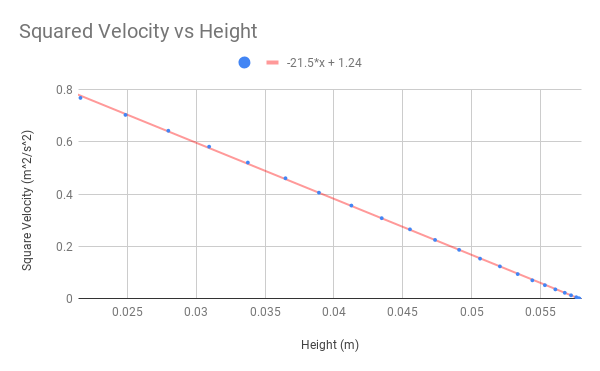
\includegraphics[scale=0.71]{image/07-mechanic/v2-uphill.png}
    \caption{$v^{2}$ versus $h$ for Run 1: Upward motion only}
    \label{figure:07.v2.1}
\end{figure}
%
\begin{figure}[ht]
    \centering
    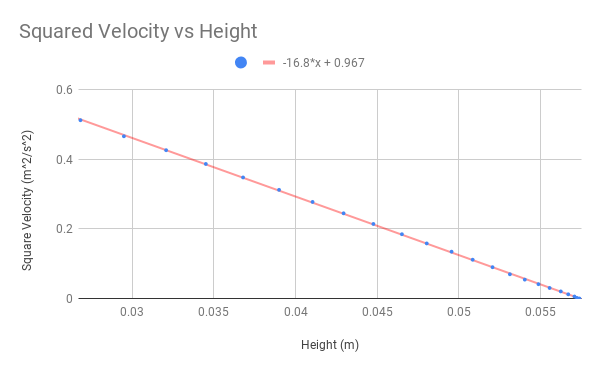
\includegraphics[scale=0.71]{image/07-mechanic/v2-downhill.png}
    \caption{$v^{2}$ versus $h$ for Run 2: Downward motion only}
    \label{figure:07.v2.2}
\end{figure}
%
\begin{figure}[ht]
    \centering
    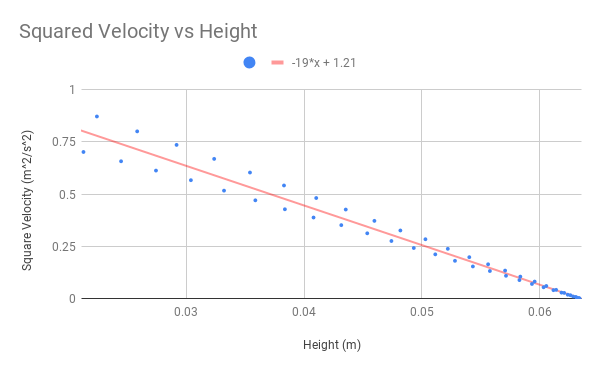
\includegraphics[scale=0.71]{image/07-mechanic/v2-both.png}
    \caption{$v^{2}$ versus $h$ for Run 3: Both upward and downward motion}
    \label{figure:07.v2.3}
\end{figure}
%
\begin{figure}[ht]
    \centering
    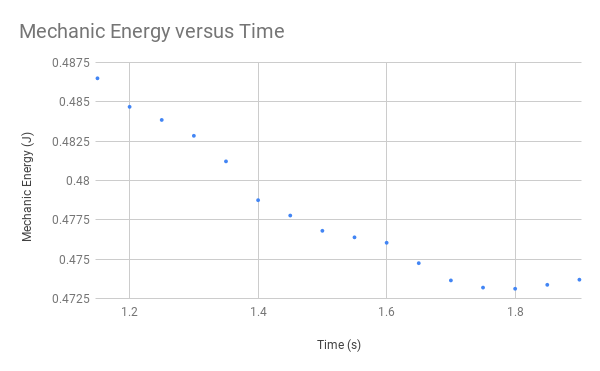
\includegraphics[scale=0.71]{image/07-mechanic/energy-4.png}
    \caption{Mechanic Energy for Run 4: Upward motion only}
    \label{figure.07.run.4.e}
\end{figure}
%
\begin{figure}[ht]
    \centering
    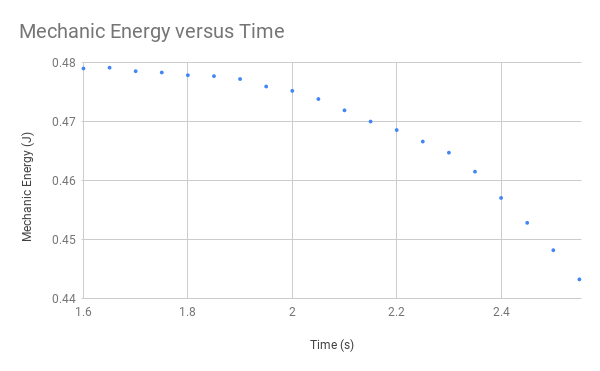
\includegraphics[scale=0.71]{image/07-mechanic/energy-5.png}
    \caption{Mechanic Energy for Run 5: Downward motion only}
    \label{figure.07.run.5.e}
\end{figure}
%
\begin{figure}[ht]
    \centering
    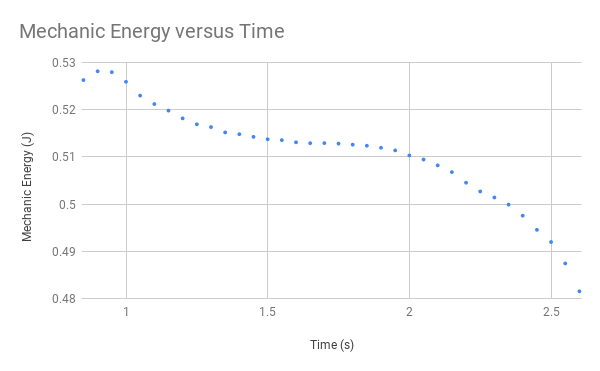
\includegraphics[scale=0.71]{image/07-mechanic/energy-6.png}
    \caption{Mechanic Energy for Run 6: Both upward and downward motion}
    \label{figure.07.run.6.e}
\end{figure}
%
\part{Momentum}
% Copyright 2018 Melvin Eloy Irizarry-Gelpí
\chapter{Impulse and Momentum}
%%%%%%%%%%%%%%%%%%%%%%%%%%%%%%%%%%%%%%%%%%%%%%%%%%%%%%%%%%%%%%%%%%%%%%%%%%%%%%%%
...
%%%%%%%%%%%%%%%%%%%%%%%%%%%%%%%%%%%%%%%%%%%%%%%%%%%%%%%%%%%%%%%%%%%%%%%%%%%%%%%%
\section{Preliminary}
%%%%%%%%%%%%%%%%%%%%%%%%%%%%%%%%%%%%%%%%%%%%%%%%%%%%%%%%%%%%%%%%%%%%%%%%%%%%%%%%
Linear momentum (or just \textbf{momentum}) is a physical quantity that incorporates velocity and mass:
\begin{equation}
    p = m v
\end{equation}
Due to the second law of motion, a net \textbf{force} causes an acceleration (a change in the velocity of an object). This in turn leads to a change in the momentum of an object. The precise relationship between momentum and forces includes a quantity called \textbf{impulse}.

Formally, impulse is defined as the area under the curve in a \textbf{force versus time} graph. In principle, we need calculus to find the area under a curve. In practice we use a simple approximation: we approximate the curve as a \textbf{flat line}. The area under a flat line has the same shape as a rectangle. The area of a rectangle is the length multiplied by the width. Which flat line to use? Since force is in the vertical axis, a flat horizontal line corresponds to a fixed value of force along time. An appropriate choice for the fixed value is the \textbf{time-averaged force} $\bar{F}$. This would correspond to the width of the rectangle. The length of the rectangle is the amount of time $\Delta t$ that the force acts. The ``area'' is thus given by
\begin{equation}
    \text{``area'' } = \bar{F} \times \Delta t = \text{ impulse}
\end{equation}
Impulse has units of force multiplying time. If force is in newtons (N) and time in seconds (s), then impulse has units of N s. However, the newton is equivalent to
\begin{equation}
    1 \text{ N} = 1 \text{ kg m/s}^{2}
\end{equation}
Thus, the N s is equivalent to
\begin{equation}
    1 \text{ N s} = 1 \text{ kg m/s}
\end{equation}
If you look carefully, these are the same units of momentum. This does not mean that impulse is the same as momentum. Indeed, impulse can also be defined as the \textbf{change in momentum}:
\begin{equation}
    \text{impulse } = p_{2} - p_{1}
\end{equation}
%%%%%%%%%%%%%%%%%%%%%%%%%%%%%%%%%%%%%%%%%%%%%%%%%%%%%%%%%%%%%%%%%%%%%%%%%%%%%%%%
\section{Experiment}
%%%%%%%%%%%%%%%%%%%%%%%%%%%%%%%%%%%%%%%%%%%%%%%%%%%%%%%%%%%%%%%%%%%%%%%%%%%%%%%%
In order to verify the relationship between momentum, force, and impulse, we need to use a mechanical system where momentum and force change with time. A cart, moving along a track and colliding with a force sensor is perfect for this. Different attachment on the force sensor allow us to study different kinds of collisions. We also use a photogate to measure the speed of the cart before and after the collision. In this way, we collect data on force, and momentum, and the impulse can be determined in two different ways.
%%%%%%%%%%%%%%%%%%%%%%%%%%%%%%%%%%%%%%%%%%%%%%%%%%%%%%%%%%%%%%%%%%%%%%%%%%%%%%%%
\section{Analysis}
%%%%%%%%%%%%%%%%%%%%%%%%%%%%%%%%%%%%%%%%%%%%%%%%%%%%%%%%%%%%%%%%%%%%%%%%%%%%%%%%
We are going to determine the amount of impulse in two different ways.
%%%%%%%%%%%%%%%%%%%%%%%%%%%%%%%%%%%%%%%%%%%%%%%%%%%%%%%%%%%%%%%%%%%%%%%%%%%%%%%%
\subsection{Impulse from Change in Momentum}
%%%%%%%%%%%%%%%%%%%%%%%%%%%%%%%%%%%%%%%%%%%%%%%%%%%%%%%%%%%%%%%%%%%%%%%%%%%%%%%%
The photogate measures the velocity of the object before the collision ($v_{1}$) and after the collision ($v_{2}$). Strictly speaking, \textbf{one of the velocities value should be negative} because there is \textbf{a change in the direction} of motion. We are going to multiply the value for $v_{2}$ by $-1$ in order to \textbf{make it negative}.

With the values of velocity, and the mass of the object, you can find the momentum of the object before the collision,
\begin{equation}
    p_{1} = m v_{1}
\end{equation}
and the momentum after the collision,
\begin{equation}
    p_{2} = m v_{2}
\end{equation}
The change in momentum is
\begin{equation}
    \Delta p = p_{2} - p_{1}
\end{equation}
This is the first estimate of the amount of impulse during the collision.
%%%%%%%%%%%%%%%%%%%%%%%%%%%%%%%%%%%%%%%%%%%%%%%%%%%%%%%%%%%%%%%%%%%%%%%%%%%%%%%%
\subsection{Impulse from Force Acting Over Time}
%%%%%%%%%%%%%%%%%%%%%%%%%%%%%%%%%%%%%%%%%%%%%%%%%%%%%%%%%%%%%%%%%%%%%%%%%%%%%%%%
The force sensor measures the amount of force on the sensor during the collision. First you need to determine when the collision is taking place. This involves making a force versus time graph and finding the time $t_{1}$ when the collision begins and the time $t_{2}$ when it ends. With these times you can compute the amount of time that the collision lasts:
\begin{equation}
    \Delta t = t_{2} - t_{1}
\end{equation}
Then you delete all the force values before and after the collision in the force column. Finally, you can compute the average force during this time period. This gives you the value of $\bar{F}$. With $\bar{F}$ and $\Delta t$ you can compute the impulse:
\begin{equation}
    \text{impulse } = \bar{F} \times \Delta t
\end{equation}
This is the second estimate of the amount of impulse during the collision.
%%%%%%%%%%%%%%%%%%%%%%%%%%%%%%%%%%%%%%%%%%%%%%%%%%%%%%%%%%%%%%%%%%%%%%%%%%%%%%%%
\section{My Data}
%%%%%%%%%%%%%%%%%%%%%%%%%%%%%%%%%%%%%%%%%%%%%%%%%%%%%%%%%%%%%%%%%%%%%%%%%%%%%%%%
There are two experiments: elastic and inelastic collisions. The difference between these experiment is that in the inelastic case, the amount of force during the collision is larger, and the velocity (and momentum) after the inelastic collision is zero. Besides that, the analysis is almost identical.
%%%%%%%%%%%%%%%%%%%%%%%%%%%%%%%%%%%%%%%%%%%%%%%%%%%%%%%%%%%%%%%%%%%%%%%%%%%%%%%%
\subsection{Elastic Collision}
%%%%%%%%%%%%%%%%%%%%%%%%%%%%%%%%%%%%%%%%%%%%%%%%%%%%%%%%%%%%%%%%%%%%%%%%%%%%%%%%
In my elastic collision data you will find 12 runs (3 for each amount of extra mass). I analyzed runs 1, 4, 7, and 10 (corresponding to no extra mass, 100 g, 200 g, and 300 g). Here are some of the steps I followed to find my results, which are in table \ref{table.08.results.elastic}.

The two values for the velocity are scattered along the velocity column. With the velocity values you can compute the momentum values, and thus the change in momentum.

The force versus time graph has to be restricted to the region where the collision is happening. This region consist of the deep well in the middle of the graph. There seems to be small oscillations after the deep well, but these are due to the fact that after the cart leaves the spring, the spring vibrates due to its elasticity. These oscillations are not part of the collision.

In order to quantify the agreement between the two values of impulse found, you can compute a modified version of the percent difference. If $I_{1}$ corresponds to the value of impulse determined from the change in momentum, and $I_{2}$ corresponds to the value of impulse determined from the average force and the length of the time interval, then the percent difference is given by
\begin{equation}
    \text{percent difference } = 200 \times \left\vert \frac{I_{1} - I_{2}}{I_{1} + I_{2}} \right\vert
\end{equation}
(The long vertical lines mean taking the absolute value and thus ignoring the sign of the fraction inside). In my case, the percent difference was always below 2\%.
%%%%%%%%%%%%%%%%%%%%%%%%%%%%%%%%%%%%%%%%%%%%%%%%%%%%%%%%%%%%%%%%%%%%%%%%%%%%%%%%
\begin{table} \label{table.08.results.elastic}
    \centering
    \begin{tabular}{|r|r|r|r|r|}\hline
        Extra mass & $\Delta p$ & Average $F$ & $\Delta t$ & Impulse \\ \hline
        0 kg & -0.339 kg m/s & -0.804 N & 0.430 s & -0.346 kg m/s \\
        0.1 kg & -0.357 kg m/s & -0.764 N & 0.476 s & -0.364 kg m/s \\
        0.2 kg & -0.528 kg m/s & -1.079 N & 0.496 s & -0.535 kg m/s \\
        0.3 kg & -0.570 kg m/s & -1.096 N & 0.528 s & -0.579 kg m/s \\
        \hline
    \end{tabular}
	\caption{Summary of results for the elastic collision}
\end{table}
%%%%%%%%%%%%%%%%%%%%%%%%%%%%%%%%%%%%%%%%%%%%%%%%%%%%%%%%%%%%%%%%%%%%%%%%%%%%%%%%
\subsection{Inelastic Collision}
%%%%%%%%%%%%%%%%%%%%%%%%%%%%%%%%%%%%%%%%%%%%%%%%%%%%%%%%%%%%%%%%%%%%%%%%%%%%%%%%
In the inelastic collisions, both the cart and the force sensor had a sticky clay attachment that enabled the cart to stick to the force sensor during the collision. Everyone has the same data, so I will not spoil the surprise. But the percent differences for the inelastic collision came out to be very small (see table \ref{table.08.results.inelastic}).

The velocity column for each inelastic collision has a single velocity measurement. This value corresponds to $v_{1}$. The velocity after the inelastic collision is zero.

There is a very important difference between the inelastic collisions and the elastic collisions: In the force versus time graph, after the initial deep well (which is deeper in the inelastic case than in the elastic case), there are peaks and wells that are significant in magnitude and cannot be regarded as noise. For example, the significant region in the force versus time graph for run 1 is in figure \ref{figure.08.run.1}. Beyond this region in time, there are further oscillations, but they are not large enough to be significant and are thus regarded as noise.
%%%%%%%%%%%%%%%%%%%%%%%%%%%%%%%%%%%%%%%%%%%%%%%%%%%%%%%%%%%%%%%%%%%%%%%%%%%%%%%%
\begin{table} \label{table.08.results.inelastic}
	\centering
    \begin{tabular}{|r|r|}\hline
        Extra mass & Percent difference \\ \hline
        0 kg & 0.355\% \\
        0.1 kg & 0.554\% \\
        0.2 kg & 0.408\% \\
        0.3 kg & 0.146\% \\
        \hline
    \end{tabular}
	\caption{Summary of results for the inelastic collision}
\end{table}
%%%%%%%%%%%%%%%%%%%%%%%%%%%%%%%%%%%%%%%%%%%%%%%%%%%%%%%%%%%%%%%%%%%%%%%%%%%%%%%%
\begin{figure} \label{figure.08.run.1}
    \centering
    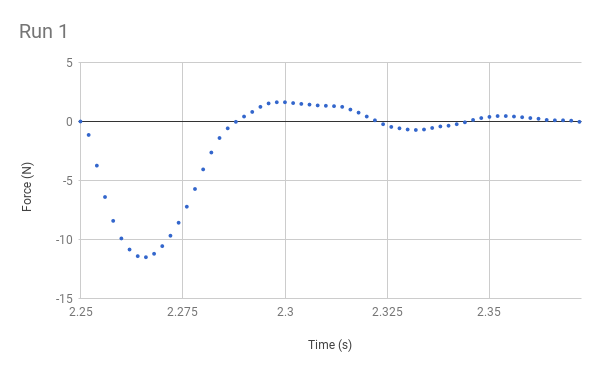
\includegraphics[scale=0.71]{image/08-impulse/run1.png}
    \caption{}
\end{figure}
%%%%%%%%%%%%%%%%%%%%%%%%%%%%%%%%%%%%%%%%%%%%%%%%%%%%%%%%%%%%%%%%%%%%%%%%%%%%%%%%
\section{Your Data}
%%%%%%%%%%%%%%%%%%%%%%%%%%%%%%%%%%%%%%%%%%%%%%%%%%%%%%%%%%%%%%%%%%%%%%%%%%%%%%%%
You collected data for elastic collisions. Everyone is going to use the same data for the inelastic case.
%%%%%%%%%%%%%%%%%%%%%%%%%%%%%%%%%%%%%%%%%%%%%%%%%%%%%%%%%%%%%%%%%%%%%%%%%%%%%%%%
\section{Your Lab Report}
%%%%%%%%%%%%%%%%%%%%%%%%%%%%%%%%%%%%%%%%%%%%%%%%%%%%%%%%%%%%%%%%%%%%%%%%%%%%%%%%
In your lab report you should include:
\begin{enumerate}
    \item A table like table \ref{table.08.results.elastic} for both the elastic and the inelastic collisions. Use these tables to answer the questions below.
    \item A table like table \ref{table.08.results.inelastic} for both the elastic and the inelastic collisions.
    \item How does the average force during the elastic collisions compare to the average force during the inelastic collision?
    \item How does the collision duration $\Delta t$ for the elastic collisions compare to the inelastic collisions?
\end{enumerate}
% Copyright 2018-2021 Melvin Eloy Irizarry-Gelpí
% Laboratory 9
\setcounter{chapter}{8}
\chapter{Collisions and Momentum}
%
In this experiment you will study momentum and kinetic energy in collisions.
%
\section{Preliminary}
%
Energy and linear momentum are very important physical quantities. These quantities can make certain problems easier to solve. One class of such problems are collisions.

Consider a system with two objects, labeled 1 and 2. Each object has a \textbf{mass} ($m_{1}$ and $m_{2}$). A collision is a very quick event where object 1 and 2 interact. Before the collision, each object has an \textbf{initial velocity} ($u_{1}$ and $u_{2}$). With the mass and the initial velocities, you can find the \textbf{initial momentum} of each object ($p_{1}$ and $p_{2}$) given by
\begin{align}
    p_{1} &= m_{1} u_{1} & p_{2} &= m_{2} u_{2}
\end{align}
Then you can find the \textbf{total initial linear momentum} $p$ given by the sum of the individual initial momenta:
\begin{equation}
    p = p_{1} + p_{2}
\end{equation}
You can also find the \textbf{initial kinetic energy} of each object ($K_{1}$ and $K_{2}$):
\begin{align}
    K_{1} &= \frac{1}{2} m_{1} \left(u_{1}\right)^{2} & K_{2} &= \frac{1}{2} m_{2} \left(u_{2}\right)^{2}
\end{align}
and the \textbf{total initial kinetic energy} $K$ given by the sum of the individual initial energies:
\begin{equation}
    K = K_{1} + K_{2}
\end{equation}
Immediately after the collision, each object has a \textbf{final velocity} ($v_{1}$ and $v_{2}$). With the mass and the final velocities, you can find the \textbf{final momentum} of each object ($q_{1}$ and $q_{2}$) given by
\begin{align}
    q_{1} &= m_{1} v_{1} & q_{2} &= m_{2} v_{2}
\end{align}
Then you can find the \textbf{total final linear momentum} $q$ given by the sum of the individual final momenta:
\begin{equation}
    q = q_{1} + q_{2}
\end{equation}
You can also find the \textbf{final kinetic energy} of each object ($L_{1}$ and $L_{2}$):
\begin{align}
    L_{1} &= \frac{1}{2} m_{1} \left(v_{1}\right)^{2} & L_{2} &= \frac{1}{2} m_{2} \left(v_{2}\right)^{2}
\end{align}
and the \textbf{total final kinetic energy} $L$ given by the sum of the individual final energies:
\begin{equation}
    L = L_{1} + L_{2}
\end{equation}
With some many quantities available, you might be having the following questions:
\begin{itemize}
    \item Are the values after the collision related to the values before the collision?
    \item Are the values associated to object 1 related to the values associated to object 2?
\end{itemize}
In a previous experiment you encountered a quantity whose value was approximately constant in time: the mechanic energy. When a cart moved along an inclined track, you saw that the value of both kinetic and gravitational energy changed with time, but the value of the sum (the mechanic energy) stayed almost constant. Back then you learned that
\begin{itemize}
    \item Energy cannot be created nor destroyed; only \textbf{converted} into other forms of energy.
\end{itemize}
That previous experiment involved a single object, the cart. A collision involves more than one object. As you are going to check, the above statement on energy can be modified to
\begin{itemize}
    \item Energy cannot be created nor destroyed; it can be \textbf{transferred} to another object or \textbf{converted} into other forms of energy.
\end{itemize}
In this experiment you will see that, in general, the total amount of momentum is conserved. However, the total amount of kinetic energy is not always conserved.
%
\section{Experiment}
%
You are going to consider three kinds of collisions:
\begin{enumerate}
    \item Elastic collisions
    \item Inelastic collisions
    \item Explosive collisions
\end{enumerate}
Each of these leads to different results.
%
\subsection{Elastic Collisions}
%
In the \textbf{elastic} collision, the objects bounce off each other after colliding. To create this effect you are going to use \textbf{repelling magnets}. The particular elastic collision you are going to study is as follows:
\begin{itemize}
    \item Before the collision, object 1 is moving towards object 2, but object 2 is at rest on the track.
    \item After the collision, object 1 might move (either backwards or forwards), and object 2 will also move.
\end{itemize}
You can change the amount of mass on each cart to see different versions.
%
\subsection{Inelastic Collisions}
%
In the \textbf{inelastic} collision, the objects stick together after colliding. To create this effect you are going to use \textbf{velcro}. The particular inelastic collision you are going to study is as follows:
\begin{itemize}
    \item Before the collision, object 1 is moving towards object 2, but object 2 is at rest on the track.
    \item After the collision, both object 1 and object 2 move together.
\end{itemize}
You can change the amount of mass on each cart to see different versions.
%
\subsection{Explosive Collisions}
%
For the \textbf{explosive} collision you are going to use the \textbf{plunger} on one of the carts. This ``collision'' is as follows:
\begin{itemize}
    \item Before the ``collision'', both objects sit at rest on the track.
    \item After the ``collision'', both objects move away from each other.
\end{itemize}
Strictly speaking, this is not a collision in the usual sense. However, if you record a video of the event and play it backwards, you would see both carts moving towards each other, colliding, and becoming at rest.

Again, you can change the amount of mass on each cart to see different versions.
%
\section{Analysis}
%
The idea is to measure the velocities of each cart and use those values to calculate the quantities mentioned above. The most difficult part is to figure out which velocity value correspond to which cart.

As a way to compare the total momentum and total kinetic energy before and after the collision, you can calculate the ratio:
\begin{align}
    \frac{q}{p} && \frac{L}{K}
\end{align}
The structure of these ratio is ``value after divided by value before collision''. If the ratio is less than one, then the value before the collision is larger, otherwise the value after the collision is larger. Note that these ratios cannot be calculated for explosive collisions.
%
\section{My Data}
%
I have three data sets:
\begin{itemize}
    \item One data set for elastic collisions.
    \item One data set for inelastic collisions.
    \item One data set for explosive collisions.
\end{itemize}
Each of these data sets has 9 runs of data:
\begin{itemize}
    \item Runs 1, 2, and 3: both carts have no extra mass.
    \item Runs 4, 5, and 6: cart 2 has 500 g of extra mass.
    \item Runs 7, 8, and 9: cart 1 has 500 g of extra mass.
\end{itemize}
There are three runs per mass variation to check for consistency. The bare total mass of each cart can be found in Table \ref{09:table.mass}.
%
\section{Your Data}
%
Your data will have the exact same structure as my data.
%
% \newpage
% \section{Your Laboratory Report}
% %
% Your lab report should include the following:
% \begin{itemize}
%     \item A table like Table \ref{09:table.mass} with the bare total mass of each cart (mass of cart plus mass of picket fence).
%     \item Tables like \ref{09:table.v.elastic}, \ref{09:table.v.inelastic}, and \ref{09:table.v.explosive} with the initial and final velocities measured, along with the particular mass values used.
%     \item Tables like \ref{09:table.p.elastic}, \ref{09:table.p.inelastic}, and \ref{09:table.p.explosive} with the initial and final momenta calculated. Also include the total initial momentum and total final momentum, as well as the ratio of the total final momentum to the total initial momentum.
%     \item Tables like \ref{09:table.K.elastic}, \ref{09:table.K.inelastic}, and \ref{09:table.K.explosive} with the initial and final kinetic energies calculated. Also include the total initial kinetic energy and total final kinetic energy, as well as the ratio of the total final kinetic energy to the total initial kinetic energy.
% \end{itemize}
% You should also answer the following questions:
% \begin{enumerate}
%     \item In general, is the total momentum before the collision ($p$) comparable to the total momentum after the collision ($q$)? When does this statement does not hold? Why?
%     \item In general, is the total kinetic energy before the collision ($K$) comparable to the total kinetic energy after the collision ($L$)? When does this statement does not hold? Why?
% \end{enumerate}
%
% \newpage
% \section{Your Laboratory Worksheet}
% %
% Please print your work before coming to class.
% %
% \paragraph{Part 1: Elastic collisions}
% %
% \begin{enumerate}
%     \item Provide a \textbf{table} with
%     \begin{itemize}
%         \item the total mass on each body ($m_{1}$ and $m_{2}$)
%         \item the velocity of each body before the collision ($u_{1}$ and $u_{2}$)
%         \item the velocity of each body after the collision ($v_{1}$ and $v_{2}$)
%     \end{itemize}
%     for each of the 3 runs considered.
%     \item Provide a \textbf{table} with
%     \begin{itemize}
%         \item the linear momentum of each body before the collision ($p_{1}$ and $p_{2}$)
%         \item the total linear momentum before the collision ($p$)
%         \item the linear momentum of each body after the collision ($q_{1}$ and $q_{2}$)
%         \item the total linear momentum after the collision ($q$)
%         \item the ratio $q/p$
%     \end{itemize}
%     for each of the 3 runs considered.
%     \item Provide a \textbf{table} with
%     \begin{itemize}
%         \item the kinetic energy of each body before the collision ($K_{1}$ and $K_{2}$)
%         \item the total kinetic energy before the collision ($K$)
%         \item the kinetic energy of each body after the collision ($L_{1}$ and $L_{2}$)
%         \item the total kinetic energy after the collision ($L$)
%         \item the ratio $L/K$
%     \end{itemize}
%     for each of the 3 runs considered.
% \end{enumerate}
% %
% \paragraph{Part 2: Inelastic collisions}
% %
% \begin{enumerate}
%     \item Provide a \textbf{table} with
%     \begin{itemize}
%         \item the total mass on each body ($m_{1}$ and $m_{2}$)
%         \item the velocity of each body before the collision ($u_{1}$ and $u_{2}$)
%         \item the velocity of each body after the collision ($v_{1}$ and $v_{2}$)
%     \end{itemize}
%     for each of the 3 runs considered.
%     \item Provide a \textbf{table} with
%     \begin{itemize}
%         \item the linear momentum of each body before the collision ($p_{1}$ and $p_{2}$)
%         \item the total linear momentum before the collision ($p$)
%         \item the linear momentum of each body after the collision ($q_{1}$ and $q_{2}$)
%         \item the total linear momentum after the collision ($q$)
%         \item the ratio $q/p$
%     \end{itemize}
%     for each of the 3 runs considered.
%     \item Provide a \textbf{table} with
%     \begin{itemize}
%         \item the kinetic energy of each body before the collision ($K_{1}$ and $K_{2}$)
%         \item the total kinetic energy before the collision ($K$)
%         \item the kinetic energy of each body after the collision ($L_{1}$ and $L_{2}$)
%         \item the total kinetic energy after the collision ($L$)
%         \item the ratio $L/K$
%     \end{itemize}
%     for each of the 3 runs considered.
% \end{enumerate}
% %
% \paragraph{Part 3: Explosive collisions}
% %
% \begin{enumerate}
%     \item Provide a \textbf{table} with
%     \begin{itemize}
%         \item the total mass on each body ($m_{1}$ and $m_{2}$)
%         \item the velocity of each body before the collision ($u_{1}$ and $u_{2}$) (each should be zero)
%         \item the velocity of each body after the collision ($v_{1}$ and $v_{2}$)
%     \end{itemize}
%     for each of the 3 runs considered.
%     \item Provide a \textbf{table} with
%     \begin{itemize}
%         \item the linear momentum of each body before the collision ($p_{1}$ and $p_{2}$) (each should be zero)
%         \item the total linear momentum before the collision ($p$) (should be zero)
%         \item the linear momentum of each body after the collision ($q_{1}$ and $q_{2}$)
%         \item the total linear momentum after the collision ($q$)
%     \end{itemize}
%     for each of the 3 runs considered.
%     \item Provide a \textbf{table} with
%     \begin{itemize}
%         \item the kinetic energy of each body before the collision ($K_{1}$ and $K_{2}$) (each should be zero)
%         \item the total kinetic energy before the collision ($K$) (should be zero)
%         \item the kinetic energy of each body after the collision ($L_{1}$ and $L_{2}$)
%         \item the total kinetic energy after the collision ($L$)
%     \end{itemize}
%     for each of the 3 runs considered.
% \end{enumerate}
% %
% \paragraph{Part 4: Results}
% %
% \begin{enumerate}
%     \item Does it make sense for the ratio $q/p$ to be larger than 1? If so, why? Otherwise, why not?
%     \item Does it make sense for the ratio $L/K$ to be larger than 1? If so, why? Otherwise, why not?
%     \item In general, is the total linear momentum before the collision ($p$) comparable to the total linear momentum after the collision ($q$)? When does this statement does not hold? Why?
%     \item In general, is the total kinetic energy before the collision ($K$) comparable to the total kinetic energy after the collision ($L$)? When does this statement does not hold? Why?
%     \item For the explosive collisions, where does the kinetic energy come from?
% \end{enumerate}
%
\newpage
\section{Example Tables}
%
\begin{table}[ht]
    \centering
    \begin{tabular}{l|r}
        \textbf{Name} & \textbf{Value} (kg) \\
        \hline
        Bare Total Mass of Cart 1 & 0.280 \\
        Bare Total Mass of Cart 2 & 0.284 \\
        \hline
    \end{tabular}
    \caption{Bare total mass values for each cart.}
    \label{09:table.mass}
\end{table}
%
\begin{table}[ht]
    \centering
    \begin{tabular}{l|r|r|r|r|r|r}
        \textbf{Run} & $m_{1}$ (kg) & $m_{2}$ (kg) & $u_{1}$ (m/s) & $u_{2}$ (m/s) & $v_{1}$ (m/s) & $v_{2}$ (m/s) \\
        \hline
        1 & & & & & & \\
        2 & & & & & & \\
        3 & & & & & & \\
        \hline
        4 & & & & & & \\
        5 & & & & & & \\
        6 & & & & & & \\
        \hline
        7 & & & & & & \\
        8 & & & & & & \\
        9 & & & & & & \\
        \hline
    \end{tabular}
    \caption{Initial and final velocities for elastic collisions}
    \label{09:table.v.elastic}
\end{table}
%
\begin{table}[ht]
    \centering
    \begin{tabular}{l|r|r|r|r|r|r}
        \textbf{Run} & $m_{1}$ (kg) & $m_{2}$ (kg) & $u_{1}$ (m/s) & $u_{2}$ (m/s) & $v_{1}$ (m/s) & $v_{2}$ (m/s) \\
        \hline
        1 & & & & & & \\
        2 & & & & & & \\
        3 & & & & & & \\
        \hline
        4 & & & & & & \\
        5 & & & & & & \\
        6 & & & & & & \\
        \hline
        7 & & & & & & \\
        8 & & & & & & \\
        9 & & & & & & \\
        \hline
    \end{tabular}
    \caption{Initial and final velocities for inelastic collisions}
    \label{09:table.v.inelastic}
\end{table}
%
\begin{table}[ht]
    \centering
    \begin{tabular}{l|r|r|r|r|r|r}
        \textbf{Run} & $m_{1}$ (kg) & $m_{2}$ (kg) & $u_{1}$ (m/s) & $u_{2}$ (m/s) & $v_{1}$ (m/s) & $v_{2}$ (m/s) \\
        \hline
        1 & & & & & & \\
        2 & & & & & & \\
        3 & & & & & & \\
        \hline
        4 & & & & & & \\
        5 & & & & & & \\
        6 & & & & & & \\
        \hline
        7 & & & & & & \\
        8 & & & & & & \\
        9 & & & & & & \\
        \hline
    \end{tabular}
    \caption{Initial and final velocities for explosive collisions}
    \label{09:table.v.explosive}
\end{table}
%
\begin{table}[ht]
    \centering
    \begin{tabular}{l|r|r|r|r|r|r|r}
        \textbf{Run} & $p_{1}$ & $p_{2}$ & $p = p_{1} + p_{2}$ & $q_{1}$ & $q_{2}$ & $q = q_{1} + q_{2}$ & $q / p$ \\
        \hline
        1 & & & & & & & \\
        2 & & & & & & & \\
        3 & & & & & & & \\
        \hline
        4 & & & & & & & \\
        5 & & & & & & & \\
        6 & & & & & & & \\
        \hline
        7 & & & & & & & \\
        8 & & & & & & & \\
        9 & & & & & & & \\
        \hline
    \end{tabular}
    \caption{Momentum for elastic collisions. All quantities are in units of kg m/s.}
    \label{09:table.p.elastic}
\end{table}
%
\begin{table}[ht]
    \centering
    \begin{tabular}{l|r|r|r|r|r|r|r}
        \textbf{Run} & $p_{1}$ & $p_{2}$ & $p = p_{1} + p_{2}$ & $q_{1}$ & $q_{2}$ & $q = q_{1} + q_{2}$ & $q / p$ \\
        \hline
        1 & & & & & & & \\
        2 & & & & & & & \\
        3 & & & & & & & \\
        \hline
        4 & & & & & & & \\
        5 & & & & & & & \\
        6 & & & & & & & \\
        \hline
        7 & & & & & & & \\
        8 & & & & & & & \\
        9 & & & & & & & \\
        \hline
    \end{tabular}
    \caption{Momentum for inelastic collisions. All quantities are in units of kg m/s.}
    \label{09:table.p.inelastic}
\end{table}
%
\begin{table}[ht]
    \centering
    \begin{tabular}{l|r|r|r|r|r|r}
        \textbf{Run} & $p_{1}$ & $p_{2}$ & $p = p_{1} + p_{2}$ & $q_{1}$ & $q_{2}$ & $q = q_{1} + q_{2}$ \\
        \hline
        1 & & & & & & \\
        2 & & & & & & \\
        3 & & & & & & \\
        \hline
        4 & & & & & & \\
        5 & & & & & & \\
        6 & & & & & & \\
        \hline
        7 & & & & & & \\
        8 & & & & & & \\
        9 & & & & & & \\
        \hline
    \end{tabular}
    \caption{Momentum for explosive collisions. All quantities are in units of kg m/s.}
    \label{09:table.p.explosive}
\end{table}
%
\begin{table}[ht]
    \centering
    \begin{tabular}{l|r|r|r|r|r|r|r}
        \textbf{Run} & $K_{1}$ & $K_{2}$ & $K = K_{1} + K_{2}$ & $L_{1}$ & $L_{2}$ & $L = L_{1} + L_{2}$ & $L / K$ \\
        \hline
        1 & & & & & & & \\
        2 & & & & & & & \\
        3 & & & & & & & \\
        \hline
        4 & & & & & & & \\
        5 & & & & & & & \\
        6 & & & & & & & \\
        \hline
        7 & & & & & & & \\
        8 & & & & & & & \\
        9 & & & & & & & \\
        \hline
    \end{tabular}
    \caption{Kinetic energy for elastic collisions. All quantities are in units of J.}
    \label{09:table.K.elastic}
\end{table}
%
\begin{table}[ht]
    \centering
    \begin{tabular}{l|r|r|r|r|r|r|r}
        \textbf{Run} & $K_{1}$ & $K_{2}$ & $K = K_{1} + K_{2}$ & $L_{1}$ & $L_{2}$ & $L = L_{1} + L_{2}$ & $L / K$ \\
        \hline
        1 & & & & & & & \\
        2 & & & & & & & \\
        3 & & & & & & & \\
        \hline
        4 & & & & & & & \\
        5 & & & & & & & \\
        6 & & & & & & & \\
        \hline
        7 & & & & & & & \\
        8 & & & & & & & \\
        9 & & & & & & & \\
        \hline
    \end{tabular}
    \caption{Kinetic energy for inelastic collisions. All quantities are in units of J.}
    \label{09:table.K.inelastic}
\end{table}
%
\begin{table}[ht]
    \centering
    \begin{tabular}{l|r|r|r|r|r|r}
        \textbf{Run} & $K_{1}$ & $K_{2}$ & $K = K_{1} + K_{2}$ & $L_{1}$ & $L_{2}$ & $L = L_{1} + L_{2}$ \\
        \hline
        1 & & & & & & \\
        2 & & & & & & \\
        3 & & & & & & \\
        \hline
        4 & & & & & & \\
        5 & & & & & & \\
        6 & & & & & & \\
        \hline
        7 & & & & & & \\
        8 & & & & & & \\
        9 & & & & & & \\
        \hline
    \end{tabular}
    \caption{Kinetic energy for explosive collisions. All quantities are in units of J.}
    \label{09:table.K.explosive}
\end{table}
%
\part{Non-Constant Acceleration}
% Copyright 2018 Melvin Eloy Irizarry-Gelpí
\setcounter{chapter}{9}
\chapter{Centripetal Motion}
%%%%%%%%%%%%%%%%%%%%%%%%%%%%%%%%%%%%%%%%%%%%%%%%%%%%%%%%%%%%%%%%%%%%%%%%%%%%%%%%
In this experiment you will study different aspects of centripetal motion.
%%%%%%%%%%%%%%%%%%%%%%%%%%%%%%%%%%%%%%%%%%%%%%%%%%%%%%%%%%%%%%%%%%%%%%%%%%%%%%%%
\section{Preliminary}
%%%%%%%%%%%%%%%%%%%%%%%%%%%%%%%%%%%%%%%%%%%%%%%%%%%%%%%%%%%%%%%%%%%%%%%%%%%%%%%%
So far, you have done experiments with objects moving in a single direction (like during free-fall motion) or back and forth (like going up and down on an inclined track, or bouncing off a spring loop). Besides such linear motion, you can have rotational motion where the direction of the motion changes continuously.

The simplest linear motion is with \textbf{constant velocity}: \textbf{uniform linear motion}. If the velocity is constant, then both its magnitude and direction are fixed in time.

The next simplest linear motion is with constant acceleration. Free-fall motion and motion on the incline are examples of this. Since acceleration is a vector quantity, constant acceleration implies constant magnitude and constant direction.

One of the simplest rotational motions is when an object moves along a \textbf{circular path} with a \textbf{velocity} vector that has a \textbf{fixed magnitude} $v$ but a direction that is constantly changing. It turns out that the \textbf{acceleration} vector of such an object also has \textbf{fixed magnitude} $a_{c}$ but constantly changing direction. The magnitude of this acceleration depends on the size of the circle and also on the magnitude of the velocity. Recall that a circle has a \textbf{radius}, which is defined as the distance from the center of the circle to any point on the circle. For an object in circular motion with constant velocity magnitude $v$ and moving in a circle with radius $r$, the magnitude of the acceleration vector is given by
\begin{equation}
    a_{c} = \frac{v^{2}}{r}
\end{equation}
This is known as the \textbf{centripetal acceleration}. If the object has mass $m$, then Newton's second law leads to the \textbf{centripetal force}:
\begin{equation}
    F_{c} = m a_{c} = \frac{m v^{2}}{r}
\end{equation}
You have sensors to measure \textbf{force} and \textbf{velocity}. The above relation suggest that for uniform circular motion you have
\begin{equation}
    F_{c} = \left(\frac{m}{r}\right) v^{2}
    \label{eq:10.Fc}
\end{equation}
That is, the amount of force acting on the object should be proportional to the square velocity. The constant of proportionality depends on the amount of \textbf{mass} and the size of the \textbf{radius} of the circle.

During uniform circular motion, the direction of the velocity vector is continuously changing. At any given moment in time, the velocity vector will be pointing in the direction that is tangential to the circle. The direction of the acceleration is also constantly changing, but it always points inwardly towards the center of the circle. Hence the name ``centripetal'' (i.e. center-pointing).
%%%%%%%%%%%%%%%%%%%%%%%%%%%%%%%%%%%%%%%%%%%%%%%%%%%%%%%%%%%%%%%%%%%%%%%%%%%%%%%%
\section{Experiment}
%%%%%%%%%%%%%%%%%%%%%%%%%%%%%%%%%%%%%%%%%%%%%%%%%%%%%%%%%%%%%%%%%%%%%%%%%%%%%%%%
The main goal of the experiment is to test the relation in (\ref{eq:10.Fc}) between the amount of force on the object and the square speed of the object. The slope depends on two quantities: mass and radius. To check this dependence, you performed two experiments:
\begin{enumerate}
    \item Keep radius fixed and change mass.
    \item Keep mass fixed and change radius.
\end{enumerate}
%%%%%%%%%%%%%%%%%%%%%%%%%%%%%%%%%%%%%%%%%%%%%%%%%%%%%%%%%%%%%%%%%%%%%%%%%%%%%%%%
\section{Analysis}
%%%%%%%%%%%%%%%%%%%%%%%%%%%%%%%%%%%%%%%%%%%%%%%%%%%%%%%%%%%%%%%%%%%%%%%%%%%%%%%%
Here are the steps to follow for the analysis.
%%%%%%%%%%%%%%%%%%%%%%%%%%%%%%%%%%%%%%%%%%%%%%%%%%%%%%%%%%%%%%%%%%%%%%%%%%%%%%%%
\subsection{Visualize Force versus Velocity}
%%%%%%%%%%%%%%%%%%%%%%%%%%%%%%%%%%%%%%%%%%%%%%%%%%%%%%%%%%%%%%%%%%%%%%%%%%%%%%%%
After each experiment you will collect velocity data from the photogate, and force data from the force sensor. It is good to make a chart with force in the vertical axis, and velocity in the horizontal axis. The chart \textbf{should not be linear}. In principle, a quadratic polynomial would be the best fit, but you do not have to do this.

You make this chart for at least one run, just to check the data.
%%%%%%%%%%%%%%%%%%%%%%%%%%%%%%%%%%%%%%%%%%%%%%%%%%%%%%%%%%%%%%%%%%%%%%%%%%%%%%%%
\subsection{Visualize Force versus Square Velocity}
%%%%%%%%%%%%%%%%%%%%%%%%%%%%%%%%%%%%%%%%%%%%%%%%%%%%%%%%%%%%%%%%%%%%%%%%%%%%%%%%
In a separate column on the spreadsheet, you can compute the square velocity values. Due to the manner in which the photogate measures velocity, the data does not consist of a velocity value for each force value. Suppose that column \texttt{B} has the force values, and column \texttt{C} has the velocity values. Suppose also that the force values begin in row \texttt{6}, such that the first force value is in cell \texttt{B6}. There is a chance that there will be no velocity value in cell \texttt{C6} (i.e. the cell is empty). The usual way to calculate the square velocity would be to write, in a separate column, something like this:
\begin{equation}
    \texttt{=C6\^{}2}
\end{equation}
and to then apply this operation to the rest of the velocity column. But since there are empty cells in the velocity column, the above operation will give zero for these empty cells. This way the square velocity column would consist of cells with square velocity values separated by cells with zero square velocity value. This is not right: for these zero square velocity values you have a corresponding non-zero force value!

You need to find the square velocity in a \textbf{conditional} way: if a cell in the velocity column is empty, then make the corresponding cell in the square velocity column also empty; otherwise calculate the square of the value. The following command accomplishes this:
\begin{equation}
    \texttt{=IF(C6="", "", C6\^{}2)}
\end{equation}
This way the square velocity column does not contain spurious zeroes.

Once the square velocity has been calculated correctly, you can make a chart with force in the vertical axis, and square velocity in the horizontal axis. The chart should now be linear. The best fit line will give you an equation of the form
\begin{equation}
    F = A v^{2} + B
\end{equation}
Here $A$ (the slope) should have units of force-divided-by-square-velocity, and $B$ (the intercept) should have units of force. If force is in N, and velocity in m/s, then $A$ should have units of
\begin{equation}
    \frac{\text{N}}{\text{m}^{2}\text{/s}^{2}} = \frac{\text{kg}}{\text{m}}
\end{equation}
and $B$ should have units of N. As discussed above, the slope of the chart should be close to the ratio of the amount of mass divided by the value of the radius. Since the intercept corresponds to the amount of force with zero velocity, the value of the intercept should be very small, corresponding to a force value that should be equivalent to noise, and thus effectively zero.
%%%%%%%%%%%%%%%%%%%%%%%%%%%%%%%%%%%%%%%%%%%%%%%%%%%%%%%%%%%%%%%%%%%%%%%%%%%%%%%%
\subsection{Cut any Plateau Region}
%%%%%%%%%%%%%%%%%%%%%%%%%%%%%%%%%%%%%%%%%%%%%%%%%%%%%%%%%%%%%%%%%%%%%%%%%%%%%%%%
For reasons that I am still trying to understand, the force sensor might yield a data set that exhibits a \textbf{plateau} (a flat region on a chart). This might be due to the force sensor saturating and not being able to properly record force data. For example, see Figure \ref{figure.10.run.1.before} where there is a plateau in the right hand side, for the larger force values. The plateau is having an undesirable effect because the linear fit is not appropriate.

It is safe to \textbf{cut the plateau} from the data set (as long as we assume the plateau is due to systematic error and not a real physical phenomenon). One way to consistently do this cut is to begin from the first row of data, and delete all the rows with a force value larger than 8 N. This is an informal \textbf{rule of thumb} and some times does not succeeds in cutting the plateau, meaning that forces less than 8 N should be cut (usually until 7.5 N). After doing such a cut, the chart should consist of a single linear segment, and the linear fit should be appropriate. For run 1, Figure \ref{figure.10.run.1} has the data after the cut. The linear fit is now much closer to the data.
%%%%%%%%%%%%%%%%%%%%%%%%%%%%%%%%%%%%%%%%%%%%%%%%%%%%%%%%%%%%%%%%%%%%%%%%%%%%%%%%
\section{My Data}
%%%%%%%%%%%%%%%%%%%%%%%%%%%%%%%%%%%%%%%%%%%%%%%%%%%%%%%%%%%%%%%%%%%%%%%%%%%%%%%%
Here is a breakdown of my runs:
\begin{itemize}
    \item Runs 1, 2, and 3: extra $m = 200$ g and $r = 10$ cm.
    \item Runs 4, 5, and 6: extra $m = 100$ g and $r = 10$ cm.
    \item Runs 7, 8, and 9: extra $m = 300$ g and $r = 10$ cm.
    \item Runs 10, 11, and 12: extra $m = 200$ g and $r = 8$ cm.
    \item Runs 13, 14, and 15: extra $m = 200$ g and $r = 12$ cm.
\end{itemize}
The corresponding expected values of the slope are found in Table \ref{table:10.m.r}.

The observed values for the slope and intercept are found in Table \ref{table:10.results}. As you can see from the second and third columns, the observed slopes are much larger than the expected values. The percent differences are consistently above 50\%, indeed closer to 60\%. Since this is true for all 15 runs, it appears that this outcome is due to a \textbf{systematic error}. Note that the slope values are consistent among repeated experiments.

This disagreement is embarrassing, but also serves as an opportunity to deal with systematic error. If you payed attention in class and repeated my steps, then very likely you found a similar disagreement in your data. Here is how I am quantifying the systematic error. Instead of the percent difference, I am going to calculate the ratio of the value of the slope that I observed from the data, to the expected value:
\begin{equation}
    \text{Ratio} = \frac{\text{Observed slope}}{\text{Expected slope}}
\end{equation}
This is done in Table \ref{table.10.ratio}. As you can see, the values in the last column are all close with an average value of 1.598. This means that, on average, the observed slope is about 1.598 times larger than the expected slope. That is, instead of getting the expected relation
\begin{equation}
    F = \left( \frac{m}{r} \right) v^{2}
\end{equation}
my data consistently implies that
\begin{equation}
    F = 1.598 \left( \frac{m}{r} \right) v^{2}
\end{equation}
There are five possible explanations for this result:
\begin{enumerate}
    \item The mass values are really 1.598 times larger than what I measured them to be. This is very unlikely.
    \item The radius values are really 1.598 times larger than what I measured them to be. This is not as unlikely, but plausible due to a bad configuration of the apparatus. Note that the radius value sets the scale for the velocity values.
    \item The force values are really 1.598 times smaller than what I measured them to be. This is puzzling, since you could expect the force measurements to disagree by an offset due to an improper zeroing, but not by a scale factor.
    \item A combination of the above effects.
    \item None of the above; something else.
\end{enumerate}
After searching online, I found a video from the makers of the equipment used in class, and it is clear that I did not followed the proper way of setting up the experiment. I still do not fully understand how any of the mistakes would lead to such a scale factor of 1.598. Last year I did not have this issue and the percent differences for the slope were very small (5\% to 15\%).

Even though there is great disagreement between the observed slope values and the expected slope values, the key facts about centripetal force were verified:
\begin{enumerate}
    \item The amount of force on an object moving in a circular path is proportional to the square velocity, as Figure \ref{figure.10.run.1} shows.
    \item When the mass of the object is increased, the slope also increases.
    \item When the mass of the object is decreased, the slope also decreases.
    \item When the radius of the circle is increased, the slope decreases.
    \item When the radius of the circle is decreased, the slope increases.
\end{enumerate}
I give myself a C- for this experiment. Sorry!
%%%%%%%%%%%%%%%%%%%%%%%%%%%%%%%%%%%%%%%%%%%%%%%%%%%%%%%%%%%%%%%%%%%%%%%%%%%%%%%%
\section{Your Data}
%%%%%%%%%%%%%%%%%%%%%%%%%%%%%%%%%%%%%%%%%%%%%%%%%%%%%%%%%%%%%%%%%%%%%%%%%%%%%%%%
You should have the following runs:
\begin{itemize}
    \item Runs 1, 2, and 3: extra $m = 200$ g and $r = 10$ cm.
    \item Runs 4, 5, and 6: extra $m = 100$ g and $r = 10$ cm.
    \item Runs 7, 8, and 9: extra $m = 300$ g and $r = 10$ cm.
    \item Runs 10, 11, and 12: extra $m = 200$ g and $r = 8$ cm.
    \item Runs 13, 14, and 15: extra $m = 200$ g and $r = 12$ cm.
\end{itemize}
The important thing about runs 7, 8 and 9 is that the extra mass value is larger than 200 g. Some students used 300 g, and others used 250 g. Both cases should yield the desirable outcome.
%%%%%%%%%%%%%%%%%%%%%%%%%%%%%%%%%%%%%%%%%%%%%%%%%%%%%%%%%%%%%%%%%%%%%%%%%%%%%%%%
\newpage
\section{Your Laboratory Report}
%%%%%%%%%%%%%%%%%%%%%%%%%%%%%%%%%%%%%%%%%%%%%%%%%%%%%%%%%%%%%%%%%%%%%%%%%%%%%%%%
Your lab report should include the following:
\begin{itemize}
    \item A table like Table \ref{table:10.m.r} with the mass values, the radii, and the expected slopes.
    \item A table like Table \ref{table:10.results} with your results.
    \item \textbf{One} chart with force in the vertical axis, and \textbf{velocity} in the horizontal axis. You are free to choose which run.
    \item \textbf{Five} charts with force in the vertical axis, and \textbf{square velocity} in the horizontal axis. One chart from runs 1, 2, or 3; one chart from runs 4, 5, or 6; one chart from runs 7, 8, or 9; one chart from runs 10, 11 or 12; and one chart from runs 13, 14, or 15. You are free to choose which five runs to include in the lab report. You should cut any plateau from the data, if present.
\end{itemize}
You should also answer the following questions:
\begin{itemize}
    \item Is the linear fit appropriate for the force versus velocity chart?
    \item Is the linear fit appropriate for the force versus square velocity chart?
    \item What happens to the observed slope when the mass is decreased?
    \item What happens to the observed slope when the mass is increased?
    \item What happens to the observed slope when the radius is decreased?
    \item What happens to the observed slope when the radius is increased?
\end{itemize}
%%%%%%%%%%%%%%%%%%%%%%%%%%%%%%%%%%%%%%%%%%%%%%%%%%%%%%%%%%%%%%%%%%%%%%%%%%%%%%%%
\newpage
\section{Tables}
%%%%%%%%%%%%%%%%%%%%%%%%%%%%%%%%%%%%%%%%%%%%%%%%%%%%%%%%%%%%%%%%%%%%%%%%%%%%%%%%
\begin{table}[ht]
    \centering
    \begin{tabular}{|l|r|r|r|r|r|}
        \hline
        Runs & Cart $m$ (kg) & Extra $m$ (kg) & Total $m$ (kg) & $r$ (m) & $m / r$ (kg/m) \\
        \hline
        1, 2, and 3 & 0.0521 & 0.2 & 0.2521 & 0.1 & 2.521 \\
        4, 5, and 6 & 0.0521 & 0.1 & 0.1521 & 0.1 & 1.521 \\
        7, 8, and 9 & 0.0521 & 0.3 & 0.3521 & 0.1 & 3.521 \\
        10, 11, and 12 & 0.0521 & 0.2 & 0.2521 & 0.08 & 3.151 \\
        13, 14, and 15 & 0.0521 & 0.2 & 0.2521 & 0.12 & 2.101 \\
        \hline
    \end{tabular}
    \caption{Mass values and radii used, along with expected slope values}
    \label{table:10.m.r}
\end{table}
%%%%%%%%%%%%%%%%%%%%%%%%%%%%%%%%%%%%%%%%%%%%%%%%%%%%%%%%%%%%%%%%%%%%%%%%%%%%%%%%
\begin{table}[ht]
    \centering
    \begin{tabular}{|l|r|r|r|r|}
        \hline
        Run & Expected Slope (kg/m) & Observed Slope (kg/m) & Intercept (N) & P.D. (\%) \\
        \hline
        1 & 2.521 & 4.1407 & -0.0583 & 64.25 \\
        2 & 2.521 & 4.0983 & -0.0493 & 62.57 \\
        3 & 2.521 & 4.0410 & -0.0135 & 60.30 \\
        \hline
        4 & 1.521 & 2.4436 & -0.0267 & 60.66 \\
        5 & 1.521 & 2.4216 & -0.0057 & 59.21 \\
        6 & 1.521 & 2.4016 & -0.0037 & 57.89 \\
        \hline
        7 & 3.521 & 5.6048 & 0.0341 & 59.18 \\
        8 & 3.521 & 5.5167 & 0.1128 & 56.68 \\
        9 & 3.521 & 5.5928 & 0.1266 & 58.84 \\
        \hline
        10 & 3.151 & 5.4076 & -0.0385 & 71.60 \\
        11 & 3.151 & 5.1893 & 0.0595 & 64.68 \\
        12 & 3.151 & 5.1779 & 0.0544 & 64.31 \\
        \hline
        13 & 2.101 & 3.2542 & 0.1626 & 54.90 \\
        14 & 2.101 & 3.2343 & 0.1480 & 53.95 \\
        15 & 2.101 & 3.1035 & 0.3134 & 47.73 \\
        \hline
    \end{tabular}
    \caption{Results for slope and intercept}
    \label{table:10.results}
\end{table}
%%%%%%%%%%%%%%%%%%%%%%%%%%%%%%%%%%%%%%%%%%%%%%%%%%%%%%%%%%%%%%%%%%%%%%%%%%%%%%%%
\begin{table}[ht]
    \centering
    \begin{tabular}{|l|r|r|r|}
        \hline
        Run & Expected Slope (kg/m) & Observed Slope (kg/m) & Ratio \\
        \hline
        1 & 2.521 & 4.141 & 1.643 \\
        2 & 2.521 & 4.098 & 1.626 \\
        3 & 2.521 & 4.041 & 1.603 \\
        \hline
        4 & 1.521 & 2.444 & 1.607 \\
        5 & 1.521 & 2.422 & 1.592 \\
        6 & 1.521 & 2.402 & 1.579 \\
        \hline
        7 & 3.521 & 5.605 & 1.592 \\
        8 & 3.521 & 5.517 & 1.567 \\
        9 & 3.521 & 5.593 & 1.588 \\
        \hline
        10 & 3.151 & 5.408 & 1.716 \\
        11 & 3.151 & 5.189 & 1.647 \\
        12 & 3.151 & 5.178 & 1.643 \\
        \hline
        13 & 2.101 & 3.254 & 1.549 \\
        14 & 2.101 & 3.234 & 1.540 \\
        15 & 2.101 & 3.104 & 1.477 \\
        \hline
    \end{tabular}
    \caption{Ratio of observed slope to expected slope}
    \label{table.10.ratio}
\end{table}
%%%%%%%%%%%%%%%%%%%%%%%%%%%%%%%%%%%%%%%%%%%%%%%%%%%%%%%%%%%%%%%%%%%%%%%%%%%%%%%%
\newpage
\section{Figures}
%%%%%%%%%%%%%%%%%%%%%%%%%%%%%%%%%%%%%%%%%%%%%%%%%%%%%%%%%%%%%%%%%%%%%%%%%%%%%%%%
\begin{figure}[ht]
    \centering
    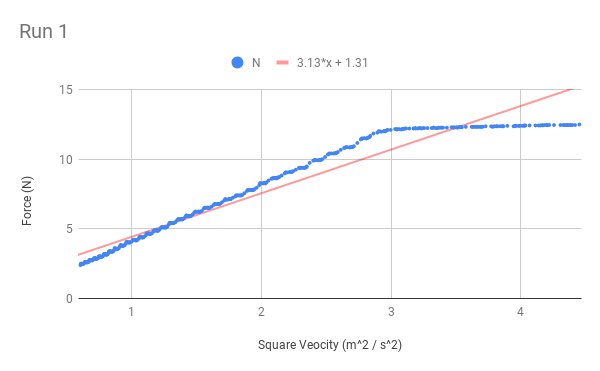
\includegraphics[scale=0.71]{image/10-centripetal/Run1BeforeCut.png}
    \caption{Run 1 before the cut; with plateau}
    \label{figure.10.run.1.before}
\end{figure}
%%%%%%%%%%%%%%%%%%%%%%%%%%%%%%%%%%%%%%%%%%%%%%%%%%%%%%%%%%%%%%%%%%%%%%%%%%%%%%%%
\begin{figure}[ht]
    \centering
    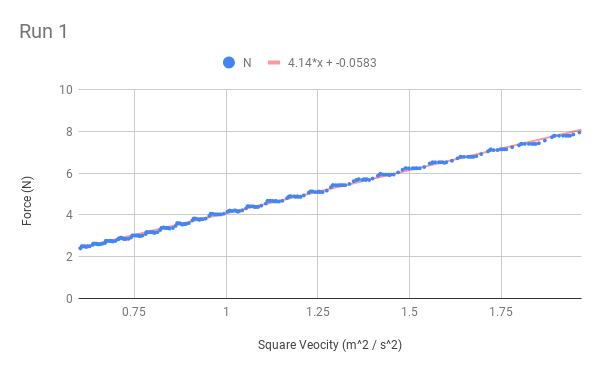
\includegraphics[scale=0.71]{image/10-centripetal/Run1.png}
    \caption{Run 1 after the cut; without plateau}
    \label{figure.10.run.1}
\end{figure}
%%%%%%%%%%%%%%%%%%%%%%%%%%%%%%%%%%%%%%%%%%%%%%%%%%%%%%%%%%%%%%%%%%%%%%%%%%%%%%%%
% Copyright 2018-2020 Melvin Eloy Irizarry-Gelpí
% Laboratory 10
\setcounter{chapter}{9}
\chapter{Simple Harmonic Motion}
%
In this experiment you will study simple harmonic motion.
%
\section{Preliminary}
%
Simple harmonic motion provides a great opportunity to test many important physical laws, some of which you have already seen in previous experiments.
%
\subsection{Hooke's Law}
%
When an elastic spring is stretched or compressed beyond its natural relaxed length, a restorative force arises on the spring that causes the spring to return to its natural relaxed length. This force is proportional to how much distance $x$ the spring is stretched:
\begin{equation} \label{eq.11.hooke}
    F_{k} = - k x
\end{equation}
This relation is known as \textbf{Hooke's law}. Here the minus sign is due to the restorative nature of the force (it is always opposite to what the spring is doing), and $k$ is the \textbf{spring constant}. If force is in newtons (N) and distance from equilibrium is in meters (m), then the spring constant has units of newton-per-meter (N/m).
%
\subsection{Newton's Second Law}
%
If a mass $m$ is attached to one end of the spring, the mass will move back-and-forth when the spring is stretched or compressed. In the absence of other forces, the net force on the object is just the force from the spring.
\begin{equation}
    F_{\text{net}} = F_{k} = -kx
\end{equation}
Due to Newton's second law, you have a relation between \textbf{force} and \textbf{acceleration}:
\begin{equation}
    F_{\text{net}} = m a
\end{equation}
Thus
\begin{equation}
    ma = -kx
\end{equation}
Or in other words:
\begin{equation}
    a = -\left( \frac{k}{m} \right) x
    \label{eq.11.ax}
\end{equation}
That is, for this back-and-forth motion, the acceleration is proportional to the amount of distance that the spring is stretched or compressed. Note that the slope is negative. If $k$ is in N/m, and $m$ is in kg, then $k/m$ will be in N / (kg m), or equivalently:
\begin{equation}
    1 \frac{\text{N}}{\text{kg m}} = 1 \frac{1}{\text{s}^{2}}
\end{equation}
Hence, the slope of the $a$ versus $x$ relation should have units of inverse square time. For convenience, you can introduce
\begin{equation}
    \omega = \sqrt{\frac{k}{m}}
\end{equation}
such that
\begin{equation}
    a = - \omega^{2} x
    \label{eq:11.axomega}
\end{equation}
The physical meaning of $\omega$ will become clear later.
%
\subsection{Sine and Cosine}
%
The \textbf{sine} and \textbf{cosine} functions are very important (and relevant) for simple harmonic motion. These functions are familiar from trigonometry where they are used to express the ratio of lengths in a right triangle.

Figure \ref{figure:11.sin.cos} shows the shape of the cosine and sine functions. These functions oscillate between $\pm 1$ and are \textbf{periodic}. More specifically, the horizontal distance between consecutive peaks of $\sin(x)$ and $\cos(x)$ is $2\pi$. Note that the ``angle'' in Figure \ref{figure:11.sin.cos} is not in degrees, but in a system of units known as \textbf{radians}. Most calculators and computers assume that the $x$ is in radians before computing sine or cosine. The conversion factor between radians and degrees is
\begin{equation}
    180 \text{ degrees} = \pi \text{ radians}
\end{equation}
The symbol for radians is rad. For all practical purposes, a radian is equivalent to a pure number without units.
%
\subsection{Sinusoidal Motion}
%
When you look at the position of the object as it changes with time, you will notice a pattern similar to a sine or cosine function. This suggest a \textbf{sinusoidal fit} for position $x$ as a function of time $t$:
\begin{equation}
    x(t) = A_{x} \sin\left( B_{x}t + C_{x} \right) + D_{x}
\end{equation}
Here $A_{x}$ is the position \textbf{amplitude} of the motion (in m), $B_{x}$ is the position \textbf{angular frequency} (in rad/s), $C_{x}$ is the position \textbf{phase shift} (in rad), and $D_{x}$ is the \textbf{position shift} (in m).

Velocity is defined as the rate of change of position with respect to time. With calculus, this is equivalent to taking a derivative of position with respect to time:
\begin{equation}
    v(t) = \frac{\mathrm{d} x}{\mathrm{d} t} = A_{x}B_{x} \cos\left( B_{x}t + C_{x} \right)
    \label{eq.11.v}
\end{equation}
That is, the fit parameters that describe the sinusoidal fit for position (i.e. $A_{x}$, $B_{x}$, $C_{x}$, and $D_{x}$) can also be used to describe the sinusoidal fit for velocity.

Similarly, acceleration is defined as the rate of change of velocity with respect to time. With calculus, this is equivalent to taking a derivative of velocity with respect to time:
\begin{equation}
    a(t) = \frac{\mathrm{d} v}{\mathrm{d} t} = -A_{x}B^{2}_{x} \sin\left( B_{x}t + C_{x} \right)
    \label{eq.11.a}
\end{equation}
Again, the parameters that describe the sinusoidal fit for position can also be used to describe the sinusoidal fit for acceleration.

As observed during the experiment, the amount of force over time also has a pattern similar to a sine or cosine function. Since force and position are different physical quantities, some of the fit parameters will have different units:
\begin{equation}
    F(t) = A_{F} \sin\left(B_{F} t + C_{F}\right) + D_{F}
\end{equation}
Here $A_{F}$ is the force \textbf{amplitude} (in N), $B_{F}$ is the force \textbf{angular frequency} (in rad/s), $C_{F}$ is the force \textbf{phase shift} (in rad), and $D_{F}$ is the \textbf{force shift} (in N).

Based on Hooke's law, you would expect some relations between the fit parameters of force and position:
\begin{equation}
    F(t) = - k x(t)
\end{equation}
This relation gives
\begin{equation}
    A_{F} \sin\left(B_{F} t + C_{F}\right) + D_{F} = -k A_{x} \sin\left( B_{x}t + C_{x} \right) - kD_{x}
\end{equation}
That is, you expect
\begin{align}
    A_{F} = kA_{x} && B_{F} = B_{x} && \vert C_{F} - C_{x} \vert = \pi && D_{F} = -kD_{x}
\end{align}
Since force and position are being measured by different sensors, these relations are non-trivial.
%
\subsection{Period of Oscillation and Angular Frequency}
%
For a mass $m$ attached to a spring with spring constant $k$, the \textbf{period of oscillation} is given by
\begin{equation}
    T = 2\pi \sqrt{\frac{m}{k}}
\end{equation}
The period is the time it takes for the mass to do one full cycle. Related to the period is the \textbf{angular frequency} $\omega$:
\begin{equation}
    \omega = \frac{2 \pi}{T} = \sqrt{\frac{k}{m}}
    \label{eq.11.omega}
\end{equation}
You have already seen the appearance of $\omega^{2}$ as the slope in the $a$ versus $x$ relation in Figure \ref{eq:11.axomega}. As you are going to see, the same value of angular frequency controls how quickly position, velocity, acceleration, and force change with time.
%
\section{Experiment}
%
You used a motion sensor to measure the position, velocity and acceleration of a mass hanging from a spring. The spring in turn hangs from a force sensor that you used to measure force. If the sensor is zeroed correctly, the constant weight force $mg$ is taken into account. When the hanging mass is moved from equilibrium and released, the motion was oscillatory.

After recording data for a short time, you used the LabQuest device to obtain the values of the fit parameters that best describe both the force and the position data versus time.

You used four combinations of mass and spring constant, as stated in Table \ref{table.11.parameters}.
%
\section{Analysis}
%
There are many aspects of simple harmonic motion that can be verified with this experiment.
%
\subsection{Force and Position}
%
You can verify \textbf{Hooke's law}, equation (\ref{eq.11.hooke}), by making a scatter chart with \textbf{position} in the horizontal axis, and \textbf{force} in the vertical axis. The shape of this chart should be a downward line, as in Figure \ref{figure.11.hooke}. You can find the slope with the \texttt{SLOPE} function. If position is in column \texttt{X} with the first value in row \texttt{6}, and force is in column \texttt{Y}, with first value in row \texttt{6}; then the command is
\begin{equation}
    \texttt{=SLOPE(Y6:Y, X6:X)}
\end{equation}
The linear behavior confirms Hooke's law. The slope of the linear fit corresponds to the (negative) value of the \textbf{spring constant}. Conversely, the negative of the slope serves as an indirect measurement of the spring constant:
\begin{equation}
    k_{\text{obs}} = - (\text{slope of force versus position linear fit})
\end{equation}
Note that position and force data come from \textbf{different} sensors.
%
\subsection{Force and Acceleration}
%
You can verify \textbf{Newton's second law of motion} by making a scatter chart with \textbf{acceleration} in the horizontal axis, and \textbf{force} in the vertical axis. The shape of this chart should be an upward line, as in Figure \ref{figure.11.newton}. You can find the slope with the \texttt{SLOPE} function. The linear behavior confirms Newton's second law, and the value of the slope is \textbf{mass}. You can use this slope as an indirect measurement of the amount of mass hanging from the spring:
\begin{equation}
    m_{\text{obs}} = \text{slope of force versus acceleration linear fit}
\end{equation}
Note that acceleration and force data come from \textbf{different} sensors.

Together with the measurement of the spring constant from the force versus position chart, you can compute an experimental estimate of the angular frequency via
\begin{equation}
    \omega_{1} = \sqrt{\frac{k_{\text{obs}}}{m_{\text{obs}}}}
\end{equation}
%
\subsection{Acceleration and Position}
%
Combining Hooke's law with Newton's second law of motion gives equation (\ref{eq.11.ax}). Using the definition of $\omega$ in equation (\ref{eq.11.omega}), we find that indeed,
\begin{equation}
    a = -\omega^{2}x
\end{equation}
That is, for simple harmonic motion, the acceleration is proportional to the position with the slope being the (negative) square angular frequency. The shape of this chart should be a downward line, as in Figure \ref{figure.11.ax}. The slope of this chart should be the negative of the squared angular frequency. This value provides another experimental estimate of the angular frequency:
\begin{equation}
    \omega_{2} = \sqrt{- (\text{slope of acceleration versus position})}
\end{equation}
%
\subsection{Common Angular Frequency}
%
From the LabQuest device, you obtained the parameters for the sinusoidal fit for both position and force. Both the $B_{x}$ parameter in the position fit, and the $B_{F}$ parameter in the force fit should correspond to the angular frequency of the simple harmonic motion. Hence, the $B_{x}$ parameter in the position fit provides another experimental estimate of the angular frequency:
\begin{equation}
    \omega_{3} = B_{x} \text{ from position fit}
\end{equation}
and the $B_{F}$ parameter from the force fit provides another experimental estimate of the angular frequency:
\begin{equation}
    \omega_{4} = B_{F} \text{ from force fit}
\end{equation}
Note that, since the data for position and force comes from different sensors, these measurements can be taken as fully independent.

In principle you can perform a sinusoidal fit on velocity and acceleration too. However, the parameters of these fits are not independent. Indeed, theoretically, they depend on the parameters for the position fit as stated in equations (\ref{eq.11.v}) and (\ref{eq.11.a}).
%
\subsection{Velocity and Position}
%
A chart with velocity and position is called a \textbf{phase space} chart. For this particular experiment with simple harmonic motion, the velocity and position data yield an \textbf{elliptical shape} (a closed orbit), as in Figure \ref{figure.11.phase}. Now you know!
%
\section{My Data}
%
My data consist of 12 runs:
\begin{itemize}
    \item Runs 1, 2, and 3: $k = 5$ N/m and $m = 50$ g.
    \item Runs 4, 5, and 6: $k = 5$ N/m and $m = 100$ g.
    \item Runs 7, 8, and 9: $k = 15$ N/m and $m = 150$ g.
    \item Runs 10, 11, and 12: $k = 15$ N/m and $m = 200$ g.
\end{itemize}
Table \ref{table.11.fit} summarizes the sinusoidal fit parameters for the position and force data. Table \ref{table.11.k.m} summarizes the experimental estimates for the spring constant and the mass. Table \ref{table.11.omega} summarizes the results for all the estimates of the angular frequency.
%
\section{Your Data}
%
You should have considered four distinct combinations of spring constant and mass, and taken at least three runs for each combination.
%
% \newpage
% \section{Your Laboratory Report}
% %
% In your lab report you should include:
% \begin{itemize}
%     \item One table like Table \ref{table.11.fit} with the fit parameters. Also include a column with the values for $\vert C_{F} - C_{x} \vert$, and a column with the values for $A_{F} / A_{x}$.
%     \item One table like Table \ref{table.11.k.m} with the observed values for the spring constant and mass.
%     \item One table like Table \ref{table.11.omega} with all the estimates of the angular frequency. Include a column with the average value, and a column with the percent difference of the average value and the expected value.
%     \item One force versus position chart with the linear fit, for a run of your choosing. See Figure \ref{figure.11.hooke}.
%     \item One force versus acceleration chart with the linear fit, for a run of your choosing. See Figure \ref{figure.11.newton}.
%     \item One acceleration versus position chart with the linear fit, for a run of your choosing. See Figure \ref{figure.11.ax}.
%     \item One velocity versus position chart for a run of your choosing. See Figure \ref{figure.11.phase}.
% \end{itemize}
% You should answer the following questions:
% \begin{enumerate}
%     \item Based on your analysis and what we saw in class, are you convinced that (for simple harmonic motion) position, velocity, acceleration, and force can all be described by sines or cosines with a common angular frequency?
%     \item Is the angular frequency parameter $B_{x}$ for the position versus time chart the same or close to the angular frequency parameter $B_{F}$ for the force versus time graph?
%     \item Can you test Newton's second law with the data from this experiment? Does the measured mass agree with the expected value used?
%     \item Can you test Hooke's law with the data from this experiment? Does the measured spring constant agree with the expected value used?
%     \item Are your four estimates of the angular frequencies close to the expected theoretical value given by (\ref{eq.11.omega}).
% \end{enumerate}
%
\newpage
\section{Your Laboratory Worksheet}
%
Please print your work before coming to class.
%
\paragraph{Part 1: Expected values}
%
\begin{enumerate}
    \item Provide a \textbf{table} with the following columns:
    \begin{itemize}
        \item The expected value of the spring constant $k$, in N/m
        \item The expected value of the hanging mass $m$, in kg
        \item The corresponding expected value of the angular frequency $\omega$, in rad/s
    \end{itemize}
    You should have four distinct combinations.
\end{enumerate}
%
\paragraph{Part 2: Hooke's law}
%
\begin{enumerate}
    \item Provide one \textbf{scatter chart} with force in the vertical axis, and position in the horizontal axis. If the data has a linear shape, then include a best-fit line and display its equation.
    \item According to Hooke's law, the (negative) slope of the best-fit line in force versus position should correspond to the observed value of the spring constant. Provide a \textbf{table} with these values (in N/m) for each run.
\end{enumerate}
%
\paragraph{Part 3: Newton's second law of motion}
%
\begin{enumerate}
    \item Provide one \textbf{scatter chart} with force in the vertical axis, and acceleration in the horizontal axis. If the data has a linear shape, then include a best-fit line and display its equation.
    \item According to Newton's second law of motion, the slope of the best-fit line in force versus acceleration should correspond to the observed value of the hanging mass. Provide a \textbf{table} with these values (in kg) for each run.
\end{enumerate}
%
\paragraph{Part 4: Harmony}
%
\begin{enumerate}
    \item Provide one \textbf{scatter chart} with acceleration in the vertical axis, and position in the horizontal axis. If the data has a linear shape, then include a best-fit line and display its equation.
    \item According to simple harmonic motion relation, the (negative) slope of the best-fit line in acceleration versus position should correspond to the observed value of the square angular frequency. Taking the square root gives you the angular frequency. Provide a \textbf{table} with these values (in rad/s) for each run.
\end{enumerate}
%
\paragraph{Part 5: Phase space}
%
\begin{enumerate}
    \item Provide one \textbf{scatter chart} with velocity in the vertical axis, and position in the horizontal axis. What shape do you get?
\end{enumerate}
%
\paragraph{Part 6: Angular frequency}
%
\begin{enumerate}
    \item Use the observed values for spring constant and mass to calculate the \textbf{first} observed value of the angular frequency ($\omega_{1}$).
    \item The \textbf{second} observed value of the angular frequency ($\omega_{2}$) is obtained from part 4, question 2.
    \item The \textbf{third} observed value of the angular frequency ($\omega_{3}$) is obtained as the $B$ coefficient in the sinusoidal fit for position versus time.
    \item The \textbf{fourth} observed value of the angular frequency ($\omega_{4}$) is obtained as the $B$ coefficient in the sinusoidal fit for the force versus time.
    \item Provide a \textbf{table} with the four observed values of the angular frequency for each run. Also include
    \begin{itemize}
        \item The average observed angular frequency
        \item The percent difference between the average and the expected value
    \end{itemize}
    \item For each of the spring/mass configurations, are all observed values of the angular frequency close to each other? Are they close to the expected value?
\end{enumerate}
%
\newpage
\section{Table Templates}
%
\begin{table}[ht!]
    \begin{center}
        \begin{tabular}{l|l|l|l}
            & Expected $k$ (N/m) & Expected $m$ (kg) & Expected $\omega$ (rad/s) \\
            \hline
            1 & & & \\
            2 & & & \\
            3 & & & \\
            4 & & & \\
            \hline
        \end{tabular}
    \end{center}
    \caption{Sample Table 1}
\end{table}
%
\begin{table}[ht!]
    \begin{center}
        \begin{tabular}{l|l|l}
            \textbf{Run} & Observed $k$ (N/m) & Observed $m$ (kg) \\
            \hline
            1 & & \\
            2 & & \\
            3 & & \\
            \hline
            4 & & \\
            5 & & \\
            6 & & \\
            \hline
            7 & & \\
            8 & & \\
            9 & & \\
            \hline
            10 & & \\
            11 & & \\
            12 & & \\
            \hline
        \end{tabular}
    \end{center}
    \caption{Sample Table 2}
\end{table}
%
\newpage
\begin{table}[ht!]
    \begin{center}
        \begin{tabular}{l|l|l|l|l|l|l|l}
            \textbf{Run} & $\omega_{1}$ & $\omega_{2}$ & $\omega_{3}$ & $\omega_{4}$ & Average $\omega$ & Expected $\omega$ & P.D. (\%) \\
            \hline
            1 & & & & & & & \\
            2 & & & & & & & \\
            3 & & & & & & & \\
            \hline
            4 & & & & & & & \\
            5 & & & & & & & \\
            6 & & & & & & & \\
            \hline
            7 & & & & & & & \\
            8 & & & & & & & \\
            9 & & & & & & & \\
            \hline
            10 & & & & & & & \\
            11 & & & & & & & \\
            12 & & & & & & & \\
            \hline
        \end{tabular}
    \end{center}
    \caption{Sample Table 3}
\end{table}
%
\newpage
\section{Example Tables}
%
\begin{table}[ht]
    \centering
    \begin{tabular}{r|r|r}
        $k$ (N/m) & $m$ (kg) & $\omega$ (rad/s) \\ \hline
        5 & 0.05 & 10 \\
        5 & 0.1 & 7.071 \\
        15 & 0.15 & 10 \\
        15 & 0.2 & 8.660 \\
        \hline
    \end{tabular}
    \caption{Four combinations of mass and spring constant, along with the expected $\omega$ value}
    \label{table.11.parameters}
\end{table}
%
\begin{table}[ht]
    \centering
    \begin{tabular}{l|r|r|r|r|r|r|r|r}
        \textbf{Units} & N & rad/s & rad & m & rad/s & rad & rad & N/m \\
        \hline
        \textbf{Run} & $A_{F}$ & $B_{F}$ & $C_{F}$ & $A_{x}$ & $B_{x}$ & $C_{x}$ & $\vert C_{F} - C_{x} \vert$ & $A_{F} / A_{x}$ \\
        \hline
        1 & 0.18702 & 10.073 & 2.9623 & 0.035833 & 10.074 & 6.1523 & 3.19 & 5.219 \\
        2 & 0.18432 & 10.08 & 5.3656 & 0.035155 & 10.081 & 2.2804 & 3.0852 & 5.243 \\
        3 & 0.14574 & 10.087 & 1.3107 & 0.027684 & 10.087 & 4.5103 & 3.1996 & 5.264 \\
        \hline
        4 & 0.39283 & 7.151 & 1.7351 & 0.074343 & 7.1509 & 4.9147 & 3.1796 & 5.284 \\
        5 & 0.44613 & 7.1512 & 2.0286 & 0.085428 & 7.1476 & 5.2144 & 3.1858 & 5.222 \\
        6 & 0.38923 & 7.1511 & 1.419 & 0.073901 & 7.1519 & 4.5973 & 3.1783 & 5.267 \\
        \hline
        7 & 0.60109 & 10.348 & 0.63061 & 0.035986 & 10.348 & 3.829 & 3.19839 & 16.703 \\
        8 & 0.78886 & 10.341 & 0.65922 & 0.047473 & 10.337 & 3.8649 & 3.20568 & 16.617 \\
        9 & 0.51888 & 10.353 & 0.73697 & 0.030912 & 10.352 & 3.9389 & 3.20193 & 16.786 \\
        \hline
        10 & 0.78128 & 8.9734 & 2.5345 & 0.046803 & 8.9733 & 5.7246 & 3.1901 & 16.693 \\
        11 & 0.89829 & 8.9709 & 3.7414 & 0.053931 & 8.9707 & 0.65011 & 3.09129 & 16.656 \\
        12 & 0.97657 & 8.9683 & 2.5984 & 0.05852 & 8.969 & 5.7868 & 3.1884 & 16.688 \\
        \hline
    \end{tabular}
    \caption{Sinusoidal fit parameters}
    \label{table.11.fit}
\end{table}
%
\begin{table}[ht]
    \centering
    \begin{tabular}{l|r|r|r|r}
        \textbf{Units} & N/m & kg & N/m & kg \\
        \hline
        \textbf{Run} & Expected $k$ & Expected $m$ & Observed $k$ & Observed $m$ \\
        \hline
        1 & 5 & 0.05 & 5.2038 & 0.0527 \\
        2 & 5 & 0.05 & 5.2371 & 0.0538 \\
        3 & 5 & 0.05 & 5.2618 & 0.0542 \\
        \hline
        4 & 5 & 0.1 & 5.2831 & 0.1061 \\
        5 & 5 & 0.1 & 5.2220 & 0.1041 \\
        6 & 5 & 0.1 & 5.2676 & 0.1056 \\
        \hline
        7 & 15 & 0.15 & 16.6495 & 0.1621 \\
        8 & 15 & 0.15 & 16.5786 & 0.1626 \\
        9 & 15 & 0.15 & 16.7589 & 0.1630 \\
        \hline
        10 & 15 & 0.2 & 16.6761 & 0.2146 \\
        11 & 15 & 0.2 & 16.6199 & 0.2154 \\
        12 & 15 & 0.2 & 16.6586 & 0.2138 \\
        \hline
    \end{tabular}
    \caption{Expected and Observed values for spring constant and mass}
    \label{table.11.k.m}
\end{table}
%
\begin{table}[ht]
    \centering
    \begin{tabular}{l|r|r|r|r|r|r|r}
        \textbf{Units} & rad/s & rad/s & rad/s & rad/s & rad/s & rad/s & \% \\
        \hline
        \textbf{Run} & Expected $\omega$ & $\omega_{1}$ & $\omega_{2}$ & $\omega_{3}$ & $\omega_{4}$ & Average $\omega$ & P.D. \\
        \hline
        1 & 10.000 & 9.9344 & 9.8570 & 10.073 & 10.074 & 9.9846 & \textminus 0.15 \\
        2 & 10.000 & 9.8671 & 9.8177 & 10.08 & 10.081 & 9.9615 & \textminus 0.39 \\
        3 & 10.000 & 9.8499 & 9.7926 & 10.087 & 10.087 & 9.9541 & \textminus 0.46 \\
        \hline
        4 & 7.071 & 7.0579 & 7.0380 & 7.151 & 7.1509 & 7.0994 & 0.40 \\
        5 & 7.071 & 7.0825 & 7.0457 & 7.1512 & 7.1476 & 7.1067 & 0.50 \\
        6 & 7.071 & 7.0626 & 7.0410 & 7.1511 & 7.1519 & 7.1017 & 0.43 \\
        \hline
        7 & 10.000 & 10.1333 & 10.0744 & 10.348 & 10.348 & 10.2259 & 2.26 \\
        8 & 10.000 & 10.0982 & 10.0632 & 10.341 & 10.337 & 10.2098 & 2.10 \\
        9 & 10.000 & 10.1410 & 10.0852 & 10.353 & 10.352 & 10.2328 & 2.33 \\
        \hline
        10 & 8.660 & 8.8159 & 8.7990 & 8.9734 & 8.9733 & 8.8904 & 2.66 \\
        11 & 8.660 & 8.7830 & 8.7682 & 8.9709 & 8.9707 & 8.8732 & 2.46 \\
        12 & 8.660 & 8.8270 & 8.7951 & 8.9683 & 8.969 & 8.8899 & 2.65 \\
        \hline
    \end{tabular}
    \caption{Experimental estimates of the angular frequency}
    \label{table.11.omega}
\end{table}
%
\FloatBarrier
\newpage
\section{Example Charts}
%
\begin{figure}[ht]
    \centering
    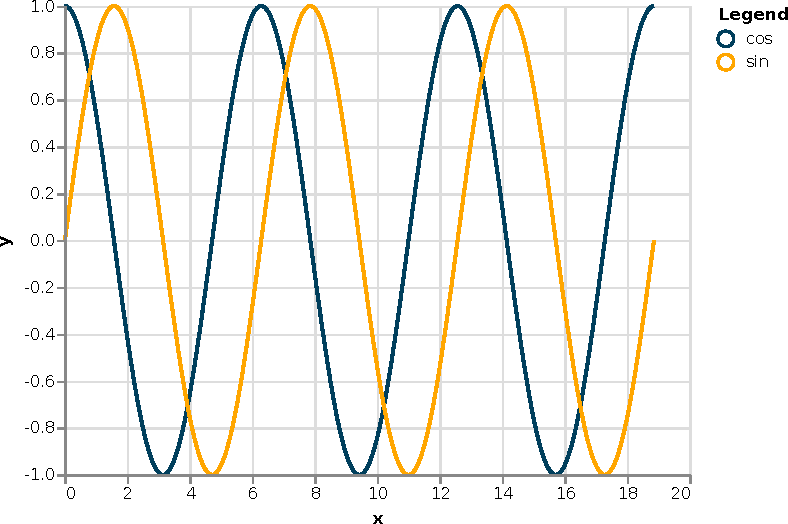
\includegraphics{chart/11-shm/trig.pdf}
    \caption{Sine and Cosine functions}
    \label{figure:11.sin.cos}
\end{figure}
%
\begin{figure}[ht]
    \centering
    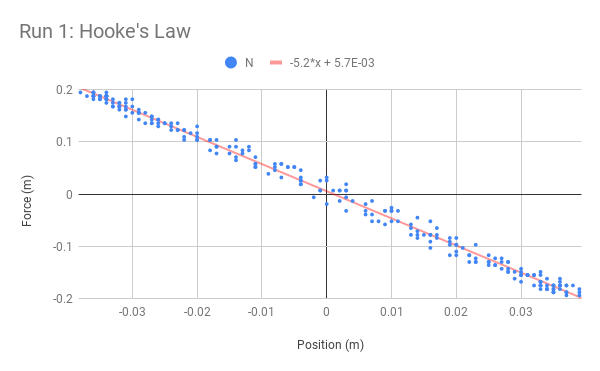
\includegraphics[scale=0.71]{image/11-shm/run-1-hooke.png}
    \caption{Testing Hooke's Law}
    \label{figure.11.hooke}
\end{figure}
%
\begin{figure}[ht]
    \centering
    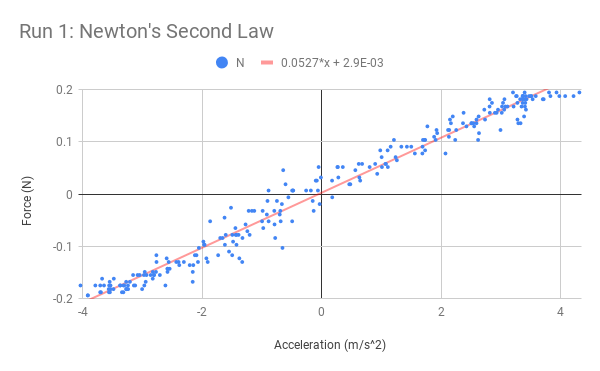
\includegraphics[scale=0.71]{image/11-shm/run-1-newton.png}
    \caption{Testing Newton's Second Law of Motion}
    \label{figure.11.newton}
\end{figure}
%
\begin{figure}[ht]
    \centering
    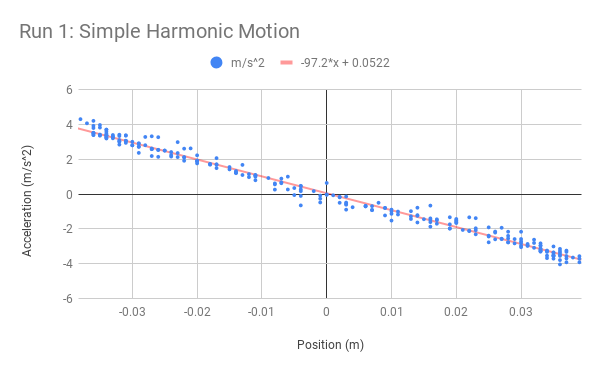
\includegraphics[scale=0.71]{image/11-shm/run-1-shm.png}
    \caption{Testing relation between acceleration and position due to simple harmonic motion}
    \label{figure.11.ax}
\end{figure}
%
\begin{figure}[ht]
    \centering
    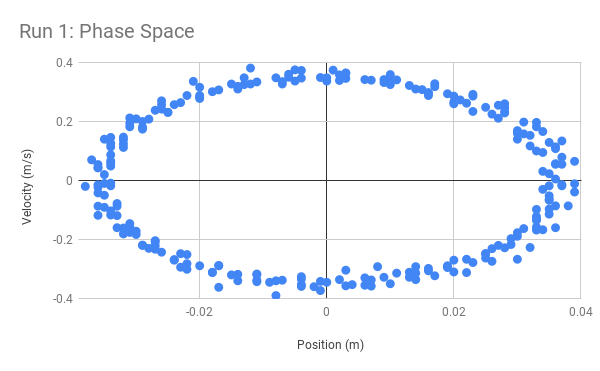
\includegraphics[scale=0.71]{image/11-shm/run-1-phase.png}
    \caption{Visualizing the phase space for simple harmonic motion}
    \label{figure.11.phase}
\end{figure}
%

%
\end{document}